\documentclass[a4paper]{report}
\usepackage[utf8]{inputenc}
\usepackage{a4wide,amssymb,epsfig,latexsym,multicol,array,hhline,fancyhdr}
\usepackage{vntex}
\usepackage{amsmath}
\usepackage{lastpage}
\usepackage[lined,boxed,commentsnumbered]{algorithm2e}
\usepackage{enumerate}
\usepackage{fancybox}
\usepackage{graphicx}
\usepackage{color}
\usepackage{colortbl}
\usepackage{listings}
\usepackage{gensymb}
\usepackage{tabularx, caption}
\usepackage{multirow}
\usepackage{rotating}
\usepackage{geometry}
\usepackage{setspace}
\usepackage{tikz}
\usepackage{enumitem}
\usepackage{tocloft}
\usepackage{etoolbox}
\usepackage{indentfirst}
\setlength{\parindent}{0.5cm}
\definecolor{dkgreen}{rgb}{0,0.6,0}
\definecolor{gray}{rgb}{0.5,0.5,0.5}
\definecolor{mauve}{rgb}{0.58,0,0.82}
\usepackage{xcolor}
\definecolor{darkblue}{RGB}{0, 51, 153}
\patchcmd{\thebibliography}{\section*{\refname}}{}{}{}
\usepackage{sectsty}

\lstset{frame=tb,
  language=Python,
  aboveskip=3mm,
  belowskip=3mm,
  showstringspaces=false,
  columns=flexible,
  basicstyle={\small\ttfamily},
  numbers=left,
  numberstyle=\tiny\color{gray},
  keywordstyle=\color{blue},
  commentstyle=\color{dkgreen},
  stringstyle=\color{mauve},
  breaklines=true,
  breakatwhitespace=true,
  tabsize=3
}
\usepackage{float}
\usepackage{subcaption}
\usepackage[section]{placeins}
\usepackage{ragged2e}
\newcolumntype{L}[1]{>{\RaggedRight\arraybackslash}p{#1}}
\newcolumntype{Y}{>{\RaggedRight\arraybackslash}X}
\raggedbottom
\setlength{\parskip}{5pt plus 1pt minus 1pt}

\usetikzlibrary{arrows,snakes,backgrounds}
\usepackage{hyperref}
\hypersetup{urlcolor=blue,linkcolor=black,citecolor=black,colorlinks=true} 

\newtheorem{theorem}{{\bf Theorem}}
\newtheorem{property}{{\bf Property}}
\newtheorem{proposition}{{\bf Proposition}}
\newtheorem{corollary}[proposition]{{\bf Corollary}}
\newtheorem{lemma}[proposition]{{\bf Lemma}}

% Chỉnh tiêu đề Mục lục (TOC)
\renewcommand{\cfttoctitlefont}{\Huge\bfseries} 
% Chỉnh tiêu đề Danh sách bảng (LOT)
\renewcommand{\cftlottitlefont}{\Huge\bfseries}
% Chỉnh tiêu đề Danh sách hình (LOF)
\renewcommand{\cftloftitlefont}{\Huge\bfseries}

\setlength{\cftaftertoctitleskip}{1cm}
\setlength{\cftafterlottitleskip}{1cm}
\setlength{\cftafterloftitleskip}{1cm}

\AtBeginDocument{\renewcommand*\contentsname{Mục lục}}
\AtBeginDocument{\renewcommand*\refname{Tài liệu tham khảo}}

\setlength{\headheight}{40pt}
\pagestyle{fancy}
\fancyhead{}
\fancyhead[L]{
 \begin{tabular}{rl}
    \begin{picture}(25,15)(0,0)
    \put(0,-8){
\includegraphics[width=8mm, height=8mm]{hcmut.png}}
   \end{picture}&
	\begin{tabular}{l}
		\textbf{\bf \ttfamily Trường Đại học Bách khoa - ĐHQG-HCM}\\
		\textbf{\bf \ttfamily Khoa Khoa học và Kỹ thuật Máy tính}
	\end{tabular} 	
 \end{tabular}
}
\fancyhead[R]{
	\begin{tabular}{l}
		\tiny \bf \\
		\tiny \bf 
	\end{tabular}  }
\fancyfoot{}
\fancyfoot[L]{\scriptsize \ttfamily Báo cáo Đồ án tốt nghiệp (CO4337) - HK2 2025 - 2026}
\fancyfoot[R]{\scriptsize \ttfamily Trang {\thepage}/\pageref{LastPage}}
\renewcommand{\headrulewidth}{0.3pt}
\renewcommand{\footrulewidth}{0.3pt}

\setcounter{secnumdepth}{4}
\setcounter{tocdepth}{3}
\makeatletter
\newcounter {subsubsubsection}[subsubsection]
\renewcommand\thesubsubsubsection{\thesubsubsection .\@alph\c@subsubsubsection}
\newcommand\subsubsubsection{\@startsection{subsubsubsection}{4}{\z@}%
                                     {-3.25ex\@plus -1ex \@minus -.2ex}%
                                     {1.5ex \@plus .2ex}%
                                     {\normalfont\normalsize\bfseries}}
\newcommand*\l@subsubsubsection{\@dottedtocline{3}{10.0em}{4.1em}}
\newcommand*{\subsubsubsectionmark}[1]{}
\makeatother

\begin{document}

\begin{titlepage}
\definecolor{bkblue}{RGB}{0,71,186}
\definecolor{bklightblue}{RGB}{100,181,246}

\begin{tikzpicture}[remember picture,overlay,inner sep=0,outer sep=0]
  \draw[bkblue,line width=3pt] 
    ([xshift=1cm,yshift=1cm]current page.south west) rectangle 
    ([xshift=-1cm,yshift=-1cm]current page.north east);
  
  \draw[bklightblue,line width=1.5pt] 
    ([xshift=1.5cm,yshift=1.5cm]current page.south west) rectangle 
    ([xshift=-1.5cm,yshift=-1.5cm]current page.north east);
\end{tikzpicture}

\begin{center}
ĐẠI HỌC QUỐC GIA THÀNH PHỐ HỒ CHÍ MINH \\
TRƯỜNG ĐẠI HỌC BÁCH KHOA \\
KHOA KHOA HỌC VÀ KỸ THUẬT MÁY TÍNH
\end{center}

\vspace{1cm}

\begin{figure}[h!]
\begin{center}

\includegraphics[width=4cm]{hcmut.png}
\end{center}
\end{figure}

\begin{center}
\begin{tabular}{c}
\multicolumn{1}{c}
{\textbf{{\large BÁO CÁO ĐỒ ÁN TỐT NGHIỆP}}}\\
\multicolumn{1}{c}
{\textbf{{\large MÃ HỌC PHẦN: CO4337}}}\\
\\
\hline
\\
\textbf{\textcolor{darkblue}{\Large PHÁT TRIỂN ỨNG DỤNG DI ĐỘNG}}\\

\textbf{\textcolor{darkblue}{\Large PHỤC VỤ NHÂN SỰ TRƯỜNG ĐẠI HỌC}}\\
\\
\hline
\\
\textbf{\large NGÀNH: KHOA HỌC MÁY TÍNH}
\end{tabular}
\end{center}

% --- Bảng 1: Danh sách Hội đồng ---
\begin{table}[h]
    \begin{tabular}{lllc}
        \hspace{3cm} & \large{GVHD}: & \large{ThS. Nguyễn Thanh Tùng} & \\
        \hspace{3cm} & \large{CTHĐ}: & \large{TS. Nguyễn Lê Duy Lai}  & \\
        \hspace{3cm} & \large{TKHĐ}: & \large{ThS. Trần Hồng Tài}     & 
    \end{tabular}
\end{table}

% --- Phần trang trí (Bông o0o) ---
\begin{center}
    \rule[0.25ex]{3.5cm}{0.5pt} \ \textbf{\large o0o} \ \rule[0.25ex]{3.5cm}{0.5pt}
\end{center}

% --- Bảng 2: Danh sách Sinh viên ---
\begin{table}[h]
    \begin{tabular}{lllc}
        \hspace{3cm} & \large{SVTH1}: & \large{Vũ Xuân Chính - 2210392} & \\
        \hspace{3cm} & \large{SVTH2}: & \large{Tống Duy Khang - 2211467} & 
    \end{tabular}
\end{table}

\vspace{2cm}
\begin{center}
{\footnotesize \large{TP. Hồ Chí Minh, năm 2026}}
\end{center}
\end{titlepage}

% trang trống
\newpage
\thispagestyle{empty}
\mbox{}

%trang lời cam đoan
\newpage
\begin{center}
\textbf{\fontsize{24}{28}\selectfont LỜI CAM ĐOAN}\\ 
\end{center}
\vspace{1cm}
Chúng tôi xin cam đoan đây là công trình nghiên cứu và hiện thực của riêng nhóm chúng tôi dưới sự hướng dẫn của ThS. Nguyễn Thanh Tùng. Mọi sao chép không hợp lệ, vi phạm quy chế đào tạo, chúng tôi hoàn toàn chịu trách nhiệm và nhận mọi hình thức kỷ luật.
\vspace{1cm}
\begin{flushright}
    NHÓM SINH VIÊN THỰC HIỆN \\
    \vspace{0.1 cm}
    \textit{Vũ Xuân Chính} \\
    \textit{Tống Duy Khang}
\end{flushright}

%trang lời cảm ơn
\newpage
\begin{center}
\textbf{\fontsize{24}{28}\selectfont LỜI CẢM ƠN}\\ 
\end{center}
\vspace{1cm}
Trước khi đi vào nội dung chi tiết của báo cáo, nhóm xin được dành hết lòng biết ơn của mình tới \textbf{ThS. Nguyễn Thanh Tùng} - giảng viên khoa Khoa học và Kỹ thuật Máy tính trường Đại học Bách Khoa TPHCM, người đã tận tình định hướng, hỗ trợ và đóng góp nhiều ý kiến chuyên môn quý báu trong suốt quá trình thực hiện đồ án tốt nghiệp. \\
\\
Bên cạnh đó, nhóm cũng xin chân thành gửi lời cảm ơn đến quý thầy cô hiện đã và đang công tác tại \textbf{Khoa Khoa học và Kỹ thuật Máy tính - Trường Đại học Bách Khoa - ĐHQG-HCM} đã truyền đạt cho nhóm nền tảng kiến thức chuyên môn và kỹ năng thực hành vững chắc trong suốt những năm học vừa qua. \\
\\
Cuối cùng, xin gửi lời cảm ơn sâu sắc đến gia đình, bạn bè đã luôn động viên, tạo điều kiện thuận lợi và đồng hành cùng nhóm để hoàn thành tốt đồ án tốt nghiệp này.
\vspace{1cm}
\begin{flushright}
    NHÓM SINH VIÊN THỰC HIỆN \\
    \vspace{0.1 cm}
    \textit{Vũ Xuân Chính} \\
    \textit{Tống Duy Khang}
\end{flushright}

%%tóm tắt
\newpage
\begin{center}
\textbf{\fontsize{24}{28}\selectfont TÓM TẮT BÁO CÁO}\\ 
\end{center}
\vspace{1cm}
Báo cáo Đồ án Tốt nghiệp đề tài \textbf{``Phát triển ứng dụng di động phục vụ nhân sự Trường Đại học''} trình bày quá trình nghiên cứu, thiết kế, hiện thực hóa và kiểm thử ứng dụng di động \textbf{MyHCMUT} tích hợp với hệ thống dịch vụ Backend hiện hữu của Nhà trường. Báo cáo được cấu trúc thành 7 chương chính như sau:
\begin{itemize}
    \item \textbf{CHƯƠNG I: GIỚI THIỆU} \\
    Giới thiệu chung về đề tài, đặt vấn đề, mục tiêu, phạm vi ranh giới nghiên cứu, chức năng chính và ý nghĩa đề tài.
    \item \textbf{CHƯƠNG II: PHÂN TÍCH CÁC HỆ THỐNG CÓ LIÊN QUAN TRÊN THỊ TRƯỜNG} \\
    Khảo sát và phân tích các hệ thống quản trị đại học, ứng dụng di động đơn phân hệ và hệ thống Web nội bộ; từ đó đánh giá ưu điểm, hạn chế và đề xuất mô hình Cổng di động tập trung.
    \item \textbf{CHƯƠNG III: CƠ SỞ LÝ THUYẾT VÀ CÔNG NGHỆ} \\
    Trình bày cơ sở lý thuyết kiến trúc, công nghệ Frontend Mobile (Flutter, Riverpod 3, Melos, GoRouter), công nghệ Backend tích hợp (Node.js, Express, Shared JWT Bridge), Cơ sở dữ liệu và công nghệ hỗ trợ (Kafka, FCM, Socket.IO).
    \item \textbf{CHƯƠNG IV: PHÂN TÍCH VÀ ĐẶC TẢ YÊU CẦU HỆ THỐNG} \\
    Xác định người dùng, ma trận phân quyền RBAC, sơ đồ use case tổng thể; phân tích và đặc tả chi tiết yêu cầu chức năng theo từng phân hệ nghiệp vụ độc lập (Auth, HRM, iOffice, Notification, KHCN) kết hợp use case, biểu đồ hoạt động và biểu đồ tuần tự; cùng các yêu cầu phi chức năng.
    \item \textbf{CHƯƠNG V: PHÂN TÍCH VÀ THIẾT KẾ HỆ THỐNG} \\
    Thiết kế Cơ sở dữ liệu (Targeted ERD, Data Dictionary), Kiến trúc hệ thống phân tầng Clean Architecture, MultiDomainAuthInterceptor, Notification Metadata và mô hình Vận hành (System Operation E2E).
    \item \textbf{CHƯƠNG VI: KẾT QUẢ HIỆN THỰC VÀ KIỂM THỬ} \\
    Hiện thực hóa giao diện và logic các phân hệ, kết quả kiểm thử Đơn vị (Unit Tests \& Coverage), Widget Tests, Integration Tests, kịch bản E2E và đánh giá định lượng hiệu năng thực nghiệm (API Benchmarks, FCM Latency, RAM/FPS).
    \item \textbf{CHƯƠNG VII: TỔNG KẾT VÀ HƯỚNG PHÁT TRIỂN} \\
    Nhận xét kết quả đạt được, ý nghĩa khoa học và thực tiễn đối với Trường ĐHBK, những hạn chế còn tồn tại và hướng phát triển tiếp theo.
\end{itemize}

\newpage
\tableofcontents
\newpage
\listoftables
\newpage
\listoffigures

%%% CHUONG 1: GIOI THIEU
\newpage
\chapter{GIỚI THIỆU}
\label{chap:gioithieu}

\chapterintro{Trong chương này, nhóm trình bày bối cảnh và bài toán của đề tìa, đồng thời xác định mục tiêu, phạm vi, phương pháp thực hiện và đóng góp của nhóm trong quá trình phát triển ứng dụng}

\section{Đặt vấn đề}
\label{sec:datvande}

Trường Đại học Bách khoa - ĐHQG-HCM hiện có quy mô hơn 1000 cán bộ, giảng viên trong đó có 667 thường xuyên di chuyển giữa 2 cơ sở (268 Lý Thường Kiệt, quận 10 và Thủ Đức) để giảng dạy, nghiên cứu và quản lý. Nhà trường đã đầu tư hệ sinh thái phần mêm quản trị trên nền tảng Web bao gồm hệ thống quản lý nhân sự (HRM), hệ thống quản văn phòng điện tử (iOffice). Các hệ thống này hoạt động hiệu quả trên máy tính văn phòng với đầy đủ chức năng, quy chuẩn nghiệp vu, tuy nhiên khi chuyển sang bối cảnh làm việc di dộng, chúng bộc lộ những hạn chế nghiêm trọng qua khảo sát thực tế. Nhóm đã xác định được 4 vấn đề cốt lõi.
\begin{itemize}
    \item \textit{Giao diện Web không tối ưu trên thiết bị di động:} Nhận sự gặp khó khăn khi truy cập vào các hệ thống HRM hoặc iOffice trên điện thoại với chữ nhỏ, menu phức tạp, phải phóng to/cuộn nhiều lần để xem nộ dung văn bản hoặc điền phiếu nghỉ phép, một số trang bị vỡ layout trên màn hình di động,\dots 
    \item \textit{Thiếu thông báo đẩy thời gian thực:} Cán bộ không nhận được thông báo  tức thời khi có các đơn nghỉ phép/công tác cần duyệt/từ chối, văn bản mới được phân công, hoặc lịch họp đột xuất thay đổi phòng/giờ, mà phải chủ động đăng nhập web để kiểm tra nhiều lần trong ngày gây bất tiện không đáng có.
    \item \textit{Hạn chế khi thực hiện phê duyệt:} Đối với các lãnh đạo đơn vị (Trưởng/Phó Khoa, Phòng) thường xuyên đi công tác hoặc họp liên tục, khi không có máy tính xách tay bên canh, các đơn từ có thể bị treo, ảnh hướng tới tiến độ công việc và quyền lợi của người lao động.
    \item \textit{Công tác điểm danh trong các buổi họp toàn trường:} Việc điểm danh thủ công làm giảm tính minh bạch, gặp nhiều hạn chế cho việc thu thập, nhập liệu, tổng hợp
\end{itemize}

Xuất phát từ những bất cập thực tiễn đó, đề tài \textbf{``Phát triển ứng dụng di động phục vụ nhân sự Trường Đại học''} được thực hiện nhằm xây dựng ứng dụng di động **MyHCMUT** (Flutter Monorepo) đóng vai trò là một Cổng giao tiếp di động tập trung, tích hợp trực tiếp với các dịch vụ Backend hiện hữu của Nhà trường.

\section{Mục tiêu của đề tài}
\label{sec:muctieu}

\subsection{Mục tiêu tổng quát}
Nghiên cứu, thiết kế và phát triển thành công ứng dụng di động đa nền tảng \textbf{MyHCMUT} trên nền tảng Flutter, phục vụ công tác quản lý nhân sự, văn phòng điện tử, điều hành nhiệm vụ, lịch họp và thông báo đẩy; đồng thời xây dựng kiến trúc tích hợp hướng API (API-based Integration Architecture) an toàn với hệ thống dịch vụ Backend hiện hữu của Trường Đại học Bách khoa -- ĐHQG-HCM.

\subsection{Mục tiêu cụ thể}
\begin{itemize}
    \item Xây dựng ứng dụng di động hỗ trợ tra cứu hồ sơ lý lịch 11 danh mục, giao diện Diff Viewer thẩm định chỉnh sửa thông tin cá nhân trực quan.
    \item Hiện thực hóa quy trình đăng ký nghỉ phép Form Wizard 4 bước kết hợp thuật toán kiểm tra ràng buộc thời gian thực (Real-time Validation); đăng ký và phê duyệt đi công tác đa cấp.
    \item Tích hợp phân hệ Văn phòng số (iOffice) hỗ trợ tra cứu văn bản đến/đi, tích hợp trình đọc PDF trực tiếp và phân phối chỉ đạo văn bản.
    \item Xây dựng phân hệ Quản lý Nhiệm vụ \& Công việc (Tasks/Missions) hỗ trợ phân loại 3 nhóm nhiệm vụ, duyệt cây đầu việc phân cấp (\texttt{outlined-tree}) và nộp báo cáo tiến độ đợt.
    \item Phát triển phân hệ Lịch công tác và Điểm danh cuộc họp thời gian thực qua WebSocket (\texttt{Socket.IO}) trong khung giờ mở trước 1 giờ.
    \item Xây dựng Trung tâm Thông báo đẩy (FCM) hỗ trợ điều hướng sâu (Deep Linking) dựa trên 4 trường Metadata có cấu trúc.
    \item Thiết lập bộ kiểm thử 4 tầng (Testing Pyramid) và cấu hình tự động hóa kiểm thử, đóng gói ứng dụng với GitLab CI Pipeline.
\end{itemize}

\section{Phạm vi đề tài}
\label{sec:phamvi}

Để đảm bảo tính minh bạch học thuật và tính khả thi trong quá trình thực hiện, phạm vi đề tài được phân định rõ ràng như sau:
\begin{itemize}
    \item \textbf{Phần Sinh viên trực tiếp phát triển mới (100\%):} Toàn bộ ứng dụng di động MyHCMUT (Flutter Monorepo, Design System Material 3 Semantic Tokens, Riverpod State, Interceptor, UI/UX 5 phân hệ, Bộ Unit/Widget Tests, CI/CD Pipeline) và các thành phần Mobile API Adapters bổ sung trên Backend (\texttt{staff\_ly\_lich\_mobile}, helper validate nghỉ phép 4 tầng trên \texttt{hrm-be}, bổ sung metadata thông báo trên \texttt{ioffice-be}).
    \item \textbf{Hệ thống Hiện hữu của Nhà trường:} Các dịch vụ nghiệp vụ HRM Core, iOffice Core, Tasks Backend, Hệ thống Cơ sở dữ liệu PostgreSQL và Cụm Kafka/Redis nội bộ của Nhà trường.
    \item \textbf{Dịch vụ Bên thứ ba tích hợp:} Máy chủ xác thực tập trung HCMUT CAS SSO / LDAP và dịch vụ Google Firebase Cloud Messaging (FCM).
    \item \textbf{Giới hạn nghiên cứu (Out of Scope / Future Works):} Không xây dựng lại toàn bộ database hay backend có sẵn của trường; Phân hệ Kê khai Khoa học Công nghệ (KHCN) và Phòng họp trực tuyến (Meetings) dừng ở mức UI Mock; Loại bỏ tích hợp Chữ ký số Viettel CA.
\end{itemize}

\section{Chức năng chính của hệ thống}
\label{sec:chucnangchinh}

Ứng dụng di động MyHCMUT được thiết kế với 5 nhóm chức năng cốt lõi:
\begin{enumerate}
    \item \textbf{Xác thực \& Quản lý Phiên (Auth):} Đăng nhập CAS SSO, Mật khẩu, lưu trữ Token an toàn trong Keychain/Keystore, tự động Silent Refresh Token khi gặp lỗi 401.
    \item \textbf{Quản lý Nhân sự (HRM):} Tra cứu lý lịch 11 nhóm, Diff Viewer so sánh sửa lý lịch, Wizard đăng ký nghỉ phép 4 bước + Validate 4 tầng, Đăng ký \& duyệt đi công tác, Phê duyệt hàng loạt (\texttt{BatchActionBar}).
    \item \textbf{Văn phòng số (iOffice):} Tra cứu văn bản đến/đi, trình xem PDF trực tiếp, phân phối chỉ đạo xử lý văn bản.
    \item \textbf{Quản lý Nhiệm vụ (Tasks/Missions):} Phân loại 3 nhóm nhiệm vụ, lọc 5 tab, chi tiết 4 tab (Tổng quan, Cây đầu việc \texttt{outlined-tree}, Báo cáo đợt, Liên kết) và Modal chi tiết việc.
    \item \textbf{Lịch công tác \& Điểm danh họp (Schedule):} Lịch tuần trường/đơn vị, Điểm danh có mặt trước giờ họp 1 giờ, Báo vắng mặt có lý do, đồng bộ dữ liệu tức thời qua WebSocket.
\end{enumerate}

\section{Ý nghĩa đề tài và Bố cục Báo cáo}
\label{sec:ynghia_bocuc}

\subsection{Ý nghĩa đề tài}
\begin{itemize}
    \item \textbf{Ý nghĩa khoa học:} Đề tài làm rõ mô hình kiến trúc tích hợp đa dịch vụ hướng API (API-based Multi-backend Integration Architecture) trong việc phát triển ứng dụng di động doanh nghiệp trên nền tảng hạ tầng phân tán sẵn có.
    \item \textbf{Ý nghĩa thực tiễn:} Đóng góp một giải pháp ứng dụng di động hoàn chỉnh cho Trường ĐHBK -- ĐHQG-HCM, giúp nâng cao hiệu quả điều hành, giảm độ trễ phê duyệt văn bản, tối ưu hóa công tác quản lý nhân sự và hiện đại hóa quy trình điểm danh cuộc họp.
\end{itemize}

\subsection{Bố cục Báo cáo}
Báo cáo Đồ án Tốt nghiệp được cấu trúc thành 8 chương:
\begin{itemize}
    \item \textbf{Chương 1: Giới thiệu} -- Đặt vấn đề, mục tiêu, phạm vi, chức năng chính và ý nghĩa đề tài.
    \item \textbf{Chương 2: Phân tích các hệ thống có liên quan trên thị trường} -- Khảo sát các hệ thống Web và App hiện hữu, đánh giá và đề xuất giải pháp.
    \item \textbf{Chương 3: Cơ sở lý thuyết và công nghệ} -- Lý thuyết kiến trúc, công nghệ Frontend Mobile, Backend tích hợp và các công nghệ hỗ trợ.
    \item \textbf{Chương 4: Phân tích yêu cầu hệ thống} -- Tác nhân, ma trận phân quyền RBAC, yêu cầu chức năng và phi chức năng.
    \item \textbf{Chương 5: Đặc tả chi tiết các use-case và biểu đồ hoạt động} -- Đặc tả 5 Use Case cốt lõi, 4 Activity Diagrams và 8 Sequence Diagrams.
    \item \textbf{Chương 6: Phân tích và thiết kế hệ thống} -- Targeted ERD, kiến trúc Clean Architecture, MultiDomainAuthInterceptor và luồng vận hành System Operation.
    \item \textbf{Chương 7: Kết quả hiện thực và kiểm thử} -- Kết quả hiện thực giao diện các phân hệ, kết quả kiểm thử 4 tầng (Unit, Widget, Integration, E2E) và số liệu Benchmark hiệu năng.
    \item \textbf{Chương 8: Tổng kết và hướng phát triển} -- Nhận xét kết quả đạt được, hạn chế và hướng mở rộng tương lai.
\end{itemize}

%%% CHUONG 2: PHAN TICH CAC HE THONG LIEN QUAN
\newpage
\chapter{PHÂN TÍCH CÁC HỆ THỐNG CÓ LIÊN QUAN}
\label{chap:hethonglienquan}

\chapterintro{Chương này khảo sát các hệ thống và giải pháp có liên quan đến bài toán xây dựng MyHCMUT Mobile. Mục tiêu của việc khảo sát không phải lựa chọn một sản phẩm HRM để thay thế các hệ thống đang vận hành tại Trường Đại học Bách khoa -- ĐHQG-HCM, mà nhằm xác định những khả năng đã được cung cấp bởi hệ thống hiện hữu, tham khảo cách các giải pháp khác hỗ trợ người dùng trên thiết bị di động, từ đó làm rõ khoảng trống mà đề tài cần giải quyết.

Việc phân tích tập trung vào các tiêu chí xuất phát trực tiếp từ phạm vi của đề tài: khả năng sử dụng trên thiết bị di động; tra cứu và cập nhật thông tin nhân sự; đăng ký và phê duyệt nghỉ phép; đăng ký và xử lý hồ sơ đi công tác; tiếp nhận và xử lý thông báo; khả năng tích hợp với hệ thống xác thực và hệ thống nghiệp vụ hiện hữu; cũng như khả năng đáp ứng các quy trình đặc thù của Nhà trường.}

\section{Nhóm ứng dụng di động doanh nghiệp và giáo dục đơn phân hệ}
\label{sec:app_don_phan_he}

Trên thị trường hiện nay, nhiều giải pháp ứng dụng di động phục vụ quản trị nhân sự và tác vụ hành chính đã được phát triển bởi các doanh nghiệp phần mềm hoặc được một số trường đại học ứng dụng thử nghiệm:

\begin{itemize}
    \item \textbf{Ứng dụng di động chuyên biệt cho Chấm công \& Nghỉ phép (như Base.vn, 1Office, Tanca):}
    \begin{itemize}
        \item \textit{Ưu điểm:} Giao diện di động được trau chuốt, hỗ trợ chấm công định vị GPS/Wi-Fi, tạo đơn xin nghỉ phép nhanh chóng và nhận thông báo đẩy tức thời.
        \item \textit{Hạn chế:} Đây là các giải pháp đóng gói thương mại (SaaS) được thiết kế cho khối doanh nghiệp tư nhân với quy trình hành chính đơn giản. Chúng không thể đáp ứng được các quy chuẩn quản lý nhân sự phức tạp của cơ quan nhà nước / đại học công lập (như tính toán quỹ phép năm theo thâm niên ngạch bậc, quy trình duyệt đơn 2 cấp có thẩm định số quyết định TCCB, và yêu cầu bảo mật dữ liệu lưu trữ nội bộ theo quy định của ĐHQG-HCM).
    \end{itemize}
    \item \textbf{Ứng dụng di động đơn phân hệ nội bộ tại một số trường đại học:}
    \begin{itemize}
        \item \textit{Ưu điểm:} Phục vụ nhanh một nhu cầu cấp bách (ví dụ chỉ xem thời khóa biểu, hoặc chỉ xem sổ tay sinh viên).
        \item \textit{Hạn chế:} Dẫn đến tình trạng phân mảnh ứng dụng (App Fragmentation), mỗi phân hệ là một app riêng biệt khiến cán bộ phải cài đặt nhiều ứng dụng và đăng nhập nhiều lần, trải nghiệm người dùng bị đứt gãy.
    \end{itemize}
\end{itemize}

\section{Nhóm hệ thống quản lý nhân sự và điều hành trên nền tảng Web (Web-based Portals)}
\label{sec:web_portals}

Tại hầu hết các trường đại học tại Việt Nam, bao gồm cả Trường Đại học Bách khoa -- ĐHQG-HCM, các quy trình nghiệp vụ cốt lõi đều được triển khai trên nền tảng Web Desktop:
\begin{itemize}
    \item \textbf{Hệ thống Quản lý Nhân sự (HRM Web):} Quản lý toàn bộ hồ sơ lý lịch cán bộ (11 danh mục), quá trình nâng bậc lương, khen thưởng, kỷ luật, quy trình nộp đơn nghỉ phép và đăng ký đi công tác.
    \item \textbf{Hệ thống Văn phòng điện tử (iOffice Web):} Quản lý sổ văn bản đến, văn bản đi, phân phối chỉ đạo văn bản, điều hành nhiệm vụ (Tasks) và lịch tuần công tác trường/đơn vị.
\end{itemize}

\noindent \textbf{Đánh giá ưu điểm và hạn chế của nhóm hệ thống Web:}
\begin{itemize}
    \item \textit{Ưu điểm:} Đáp ứng đầy đủ, chặt chẽ tất cả các quy chuẩn nghiệp vụ quản trị nhà trường; cơ sở dữ liệu quan hệ PostgreSQL lưu trữ tập trung, an toàn và toàn vẹn giao dịch (ACID).
    \item \textit{Hạn chế:} Giao diện Web Desktop được thiết kế với nhiều bảng biểu phức tạp, không tối ưu cho màn hình cảm ứng di động; không có cơ chế gửi thông báo đẩy (Push Notifications) về điện thoại cán bộ khi có việc khẩn; không hỗ trợ hoạt động ngoại tuyến và không tận dụng được các tính năng phần cứng của điện thoại (như điểm danh họp thời gian thực qua WebSocket).
\end{itemize}

\section{Đánh giá chung và Đề xuất giải pháp}
\label{sec:danhgiachung_dexuat}

\begin{table}[H]
    \centering
    \renewcommand{\arraystretch}{1.3}
    \begin{tabularx}{\textwidth}{|p{3.5cm}|X|X|X|}
    \hline
    \textbf{Tiêu chí Đánh giá} & \textbf{App Thương mại (SaaS)} & \textbf{Hệ thống Web Nội bộ} & \textbf{Giải pháp MyHCMUT Đề xuất} \\
    \hline
    \textbf{Phù hợp Quy chế ĐHBK} & Thấp, không tùy biến được quy trình duyệt TCCB. & Tuyệt đối (100\% đúng nghiệp vụ nhà trường). & Tuyệt đối (Tích hợp trực tiếp dữ liệu Backend trường). \\
    \hline
    \textbf{Trải nghiệm Di động (Mobile UX)} & Cao, giao diện mượt mà trên smartphone. & Kém, giao diện web bị vỡ và chữ nhỏ trên mobile. & Cao (Flutter Native UI, Material 3 Design System). \\
    \hline
    \textbf{Tính Tập trung (Unified)} & Phân mảnh, chỉ có tính năng chấm công/nghỉ phép. & Tách rời giữa các trang Web HRM và iOffice riêng. & Tập trung 100\% (HRM, iOffice, Tasks, Schedule trên 1 App). \\
    \hline
    \textbf{Bảo mật Dữ liệu Nội bộ} & Rủi ro (dữ liệu lưu trên Cloud bên thứ ba). & Cao (lưu trữ trên cụm máy chủ nội bộ trường). & Tuyệt đối (Giao tiếp bảo mật nội bộ qua Shared JWT). \\
    \hline
    \end{tabularx}
    \caption{\textit{Bảng so sánh tổng hợp các giải pháp hiện có và giải pháp đề xuất}}
    \label{tab:compare_solutions}
\end{table}

\noindent \textbf{$\rightarrow$ Đề xuất Giải pháp:}  
Từ phân tích trên, giải pháp tối ưu nhất là xây dựng **Ứng dụng Di động Cổng Giao tiếp Tập trung (Unified Mobile Portal) - MyHCMUT**. Ứng dụng này không thay thế Backend hiện hữu mà đóng vai trò là một lớp giao diện di động hiện đại (Integration Layer), kết nối an toàn với các dịch vụ Backend của Nhà trường thông qua REST API, Kafka Event Streaming và WebSocket, mang lại trải nghiệm làm việc số toàn diện cho cán bộ giảng viên.

%%% CHUONG 3: CO SO LY THUYET VA CONG NGHE
\newpage
\chapter{CƠ SỞ LÝ THUYẾT VÀ CÔNG NGHỆ}
\label{chap:cosolythuyet}

Trong chương này, nhóm trình bày các nền tảng lý thuyết kiến trúc phần mềm, phân tích và so sánh chi tiết các công nghệ phát triển ứng dụng di động phía Client (Flutter, Riverpod 3, Melos Monorepo, GoRouter, Dio, SQLite), cùng cơ sở công nghệ của hệ thống Backend hiện hữu phục vụ tích hợp đa dịch vụ (Node.js Express, Shared Secret JWT, PostgreSQL, Apache Kafka, Firebase FCM và WebSocket Socket.IO).

\newpage
\section{Cơ sở lý thuyết}
\label{sec:coso_lythuyet}

\subsection{Mô hình kiến trúc phân lớp sạch (Clean Architecture)}
Kiến trúc Phân lớp Sạch (Clean Architecture) do Robert C. Martin đề xuất nhằm mục đích phân tách mã nguồn thành các lớp độc lập với nguyên tắc phụ thuộc hướng vào trong (Dependency Rule). Đối với ứng dụng di động doanh nghiệp có quy mô lớn, kiến trúc này mang lại các lợi ích cốt lõi:
\begin{itemize}
    \item \textbf{Độc lập với framework và giao diện:} Logic nghiệp vụ không bị ràng buộc vào các widget hiển thị của Flutter, cho phép dễ dàng tái cấu trúc giao diện mà không ảnh hưởng đến quy tắc xử lý dữ liệu.
    \item \textbf{Dễ dàng kiểm thử (Testability):} Tầng nghiệp vụ (Domain) và Tầng dữ liệu (Data) có thể được kiểm thử độc lập thông qua Mock Repositories mà không cần khởi chạy môi trường giao diện người dùng.
    \item \textbf{Độc lập với nguồn dữ liệu:} Ứng dụng có thể dễ dàng chuyển đổi hoặc kết hợp giữa Local Cache (SQLite / Secure Storage) và Remote Data Source (Dio HTTP Client) một cách minh bạch.
\end{itemize}

\subsection{Kiến trúc RESTful API và giao thức HTTPS}
REST (Representational State Transfer) là kiến trúc giao tiếp chuẩn hóa giữa Client và Server dựa trên giao thức HTTP không trạng thái (Stateless). Ứng dụng MyHCMUT sử dụng các phương thức HTTP chuẩn:
\begin{itemize}
    \item \texttt{GET}: Truy vấn dữ liệu (danh sách văn bản, lịch trình, lý lịch cán bộ).
    \item \texttt{POST}: Tạo mới bản ghi hoặc kích hoạt xử lý nghiệp vụ (nộp đơn nghỉ phép, điểm danh họp).
    \item \texttt{PUT / PATCH}: Cập nhật thông tin (duyệt đơn nghỉ phép, sửa lý lịch).
    \item \texttt{DELETE}: Xóa hoặc hủy yêu cầu.
\end{itemize}
Mọi luồng truyền tin giữa ứng dụng di động và máy chủ đều được mã hóa bằng giao thức HTTPS/TLS đảm bảo an toàn thông tin, chống nghe lén và tấn công Man-in-the-Middle (MITM).

\subsection{Quản lý phiên và cơ chế Shared Secret JWT Bridge}
Trong môi trường ứng dụng di động phân tán giao tiếp đồng thời với 3 dịch vụ Backend độc lập (\texttt{myhcmut-be}, \texttt{hrm-be}, \texttt{ioffice-be}), cơ chế xác thực đóng vai trò sống còn:
\begin{enumerate}
    \item \textbf{Cơ chế JSON Web Token (JWT - RFC 7519):} Chuỗi Token mã hóa chứa thông tin định danh cán bộ (\texttt{id}, \texttt{username}, \texttt{shcc}, \texttt{maDonVi}, \texttt{roles}, \texttt{permissions}).
    \item \textbf{Shared Secret JWT Bridge:} Thay vì mỗi Backend phải gửi request xác thực chéo về Auth Server mỗi khi nhận một request từ Mobile, tất cả các dịch vụ Backend của Nhà trường cùng chia sẻ chung một khóa bí mật (\texttt{AUTH\_JWT\_SECRET}). Khi Mobile gửi Token kèm Header \texttt{Authorization: Bearer <token>}, từng dịch vụ Backend tự giải mã và xác thực Token cục bộ chỉ trong vòng dưới 5ms, triệt tiêu hoàn toàn điểm nghẽn hiệu năng (Bottleneck).
    \item \textbf{Cơ chế Dual-Token và Tự động Làm mới (Silent Refresh):} Access Token có thời hạn ngắn (Short-lived) để đảm bảo an toàn, kết hợp với Refresh Token dài hạn lưu trữ mã hóa trong Keychain/Keystore. Khi Access Token hết hạn, Interceptor của ứng dụng di động tự động gọi endpoint làm mới token ở tầng nền mà không làm gián đoạn phiên làm việc của người dùng.
\end{enumerate}
\newpage
\section{Công nghệ Frontend (Mobile Client Stack)}
\label{sec:frontend_tech}

\subsection{Nền tảng Flutter \& Ngôn ngữ Dart}
Flutter là bộ công cụ phát triển ứng dụng đa nền tảng mã nguồn mở do Google phát triển. Flutter sử dụng ngôn ngữ lập trình Dart với cơ chế kiểm tra kiểu dữ liệu nghiêm ngặt (Sound Null Safety) và biên dịch AOT (Ahead-of-Time) trực tiếp sang mã máy C/C++, tự vẽ giao diện bằng Impeller/Skia Engine mà không phụ thuộc vào OEM widgets gốc.

\begin{table}[H]
    \centering
    \renewcommand{\arraystretch}{1.3}
    \begin{tabularx}{\textwidth}{|p{3cm}|X|X|X|}
    \hline
    \textbf{Tiêu chí So sánh} & \textbf{Native (Kotlin/Swift)} & \textbf{React Native} & \textbf{Flutter (Google)} \\
    \hline
    \textbf{Cơ chế biên dịch \& Render} & Biên dịch Native trực tiếp cho từng hệ điều hành. & Chạy mã JavaScript qua tầng cầu nối JavaScript Bridge. & Biên dịch AOT sang mã máy C/C++, tự vẽ giao diện bằng Impeller Engine. \\
    \hline
    \textbf{Hiệu năng Khung hình} & Cực cao, ổn định 60--120 FPS. & Có thể bị giảm FPS hoặc nghẽn bridge khi dữ liệu I/O lớn. & Cực cao, duy trì ổn định 60 FPS khi cuộn danh sách lớn. \\
    \hline
    \textbf{Tính nhất quán Giao diện} & Phụ thuộc vào UI Components gốc của từng OS. & Giao diện ánh xạ Native Widgets, có thể sai lệch giữa các OS. & Nhất quán 100\% trên cả Android và iOS nhờ cơ chế Widget riêng. \\
    \hline
    \textbf{Chi phí \& Tốc độ Phát triển} & Cao, cần 2 đội ngũ phát triển và bảo trì riêng biệt. & Nhanh, dùng chung mã nguồn JavaScript/TypeScript. & Nhanh, dùng chung mã nguồn Dart, hỗ trợ Stateful Hot Reload tức thì. \\
    \hline
    \end{tabularx}
    \caption{\textit{Bảng so sánh lựa chọn nền tảng phát triển ứng dụng di động}}
    \label{tab:compare_mobile}
\end{table}

\noindent \textbf{$\rightarrow$ Kết luận:} Nhóm lựa chọn **Flutter** để phát triển ứng dụng MyHCMUT.

\subsection{Quản lý Trạng thái: Riverpod 3}
Riverpod 3 là giải pháp quản lý trạng thái an toàn biên dịch (Compile-safe), hiện đại và mạnh mẽ nhất trong hệ sinh thái Flutter:

\begin{table}[H]
    \centering
    \renewcommand{\arraystretch}{1.3}
    \begin{tabularx}{\textwidth}{|p{3cm}|X|X|X|}
    \hline
    \textbf{Tiêu chí So sánh} & \textbf{Provider} & \textbf{BLoC (Business Logic Component)} & \textbf{Riverpod 3 (Được chọn)} \\
    \hline
    \textbf{Tính an toàn biên dịch} & Thấp, dễ gặp lỗi \texttt{ProviderNotFoundException} lúc runtime. & Cao, kiểm soát chặt chẽ qua Events và States. & Tuyệt đối (Compile-time safe), bắt lỗi phụ thuộc ngay khi biên dịch. \\
    \hline
    \textbf{Phụ thuộc BuildContext} & Bắt buộc phải có \texttt{BuildContext} trong cây Widget. & Yêu cầu \texttt{BuildContext} để đọc BlocProvider. & Hoàn toàn không phụ thuộc \texttt{BuildContext}, đọc state từ bất kỳ đâu. \\
    \hline
    \textbf{Xử lý Dữ liệu Bất đồng bộ} & Thủ công, cần tự viết cờ \texttt{isLoading}, \texttt{error}. & Cần định nghĩa nhiều class State (\texttt{Loading}, \texttt{Loaded}, \texttt{Error}). & Chuẩn hóa hoàn hảo qua \texttt{AsyncValue} (\texttt{loading}, \texttt{data}, \texttt{error}). \\
    \hline
    \textbf{Quản lý Bộ nhớ (RAM)} & Thủ công gọi \texttt{dispose()}. & Cần đóng các StreamControllers thủ công. & Tự động hủy và giải phóng bộ nhớ khi rời màn hình với \texttt{.autoDispose}. \\
    \hline
    \end{tabularx}
    \caption{\textit{Bảng so sánh các giải pháp Quản lý Trạng thái trong Flutter}}
    \label{tab:compare_state}
\end{table}

\subsection{Điều hướng trong Flutter với \texttt{go\_router}}
Nhóm sử dụng thư viện **GoRouter** hỗ trợ Declarative URL-based Routing, tích hợp cơ chế kiểm tra quyền truy cập (Route Guards) và phân giải Deep Linking từ thông báo đẩy FCM trực tiếp vào màn hình chi tiết.

\subsection{Kiến trúc Đa gói Modular Monorepo với Melos}
\begin{table}[H]
    \centering
    \renewcommand{\arraystretch}{1.3}
    \begin{tabularx}{\textwidth}{|p{3cm}|X|X|}
    \hline
    \textbf{Tiêu chí} & \textbf{Single Package (Nguyên khối)} & \textbf{Modular Monorepo với Melos (Được chọn)} \\
    \hline
    \textbf{Cấu trúc Mã nguồn} & Toàn bộ code nằm trong một thư mục \texttt{lib/} duy nhất. & Chia tách thành các Core Packages và Feature Modules riêng biệt. \\
    \hline
    \textbf{Tính Tái sử dụng} & Khó tái sử dụng Design System hoặc Network Client. & Gói \texttt{global\_system} và \texttt{network} được chia sẻ cho mọi module. \\
    \hline
    \textbf{Phụ thuộc vòng} & Dễ xảy ra import chéo, gây phụ thuộc vòng lộn xộn. & Phân tầng nghiêm ngặt: Feature Module chỉ phụ thuộc Core Packages. \\
    \hline
    \textbf{Tự động hóa CI/CD} & Chạy test toàn bộ dự án dù chỉ sửa một dòng code. & Chạy phân tích tĩnh, định dạng và kiểm thử độc lập cho từng module. \\
    \hline
    \end{tabularx}
    \caption{\textit{Bảng so sánh kiến trúc cấu trúc dự án Monorepo và Single Package}}
    \label{tab:compare_monorepo}
\end{table}

\subsection{Quản lý Yêu cầu HTTP và Bộ nhớ đệm Cục bộ}
\begin{itemize}
    \item \textbf{Dio HTTP Client:} Hỗ trợ Interceptors gắn token tự động, thiết lập Timeout và chuyển đổi JSON.
    \item \textbf{Flutter Secure Storage:} Lưu trữ an toàn Token trong iOS Keychain và Android Keystore.
    \item \textbf{SQLite (sqflite):} Bộ nhớ đệm cục bộ lưu danh mục tĩnh (Master Data) để hỗ trợ hiển thị tức thì.
\end{itemize}

\newpage
\section{Công nghệ Backend, Quản lý Tương tranh và Tích hợp Đa dịch vụ}
\label{sec:backend_tech}

Mục này trình bày cơ sở công nghệ của hệ thống Backend hiện hữu phục vụ tích hợp đa dịch vụ, phân tích chuyên sâu các bài toán kỹ thuật cốt lõi mà nhóm sinh viên trực tiếp can thiệp giải quyết: quản trị giao dịch và kiểm soát tương tranh trong cơ sở dữ liệu, đường ống phân phối thông báo bất đồng bộ qua Apache Kafka, cùng cơ chế chuyển tiếp xác thực an toàn qua Single Sign-On (SSO) Bridge.

\subsection{Tổng quan Kiến trúc Backend Kế thừa của Nhà trường}
\label{subsec:legacy_backend_overview}

Hệ thống dịch vụ quản trị của Trường Đại học Bách khoa -- ĐHQG-HCM vận hành theo mô hình kiến trúc phân tầng (Layered Architecture):
\begin{itemize}
    \item \textbf{Môi trường thực thi Node.js \& TypeScript:} Xử lý I/O bất đồng bộ (Non-blocking I/O) theo mô hình Event Loop đơn luồng, kết hợp cùng TypeScript đảm bảo an toàn kiểu dữ liệu.
    \item \textbf{Web Framework Express.js:} Cung cấp cơ chế định tuyến RESTful API và chuỗi Middleware kiểm soát phiên, giải mã token và phân quyền RBAC.
    \item \textbf{Hệ quản trị Cơ sở dữ liệu PostgreSQL \& Sequelize ORM:} Lưu trữ toàn bộ dữ liệu viên chức, lịch cá nhân và quy trình duyệt. Sequelize ORM quản lý mô hình ánh xạ đối tượng và điều khiển giao dịch CSDL (\texttt{Sequelize.Transaction}).
\end{itemize}

\subsection{Bài toán Kiểm soát Tương tranh và Lập luận Lựa chọn Giải pháp Khóa (Concurrency Control)}
\label{subsec:concurrency_reasoning}

\subsubsection{Hiện tượng Cạnh tranh Đăng ký Trùng lịch (Double-Booking Anomaly)}
Trong phân hệ đăng ký nghỉ phép và lịch công tác, một yêu cầu nộp đơn hợp lệ phải thỏa mãn điều kiện không trùng khoảng thời gian với các lịch đã tồn tại của cùng một nhân sự (\texttt{shcc}). Quá trình này bao gồm hai bước logic:
\begin{enumerate}
    \item \textit{Đọc và kiểm tra (Check):} Truy vấn bảng \texttt{tcns\_lich\_ca\_nhan} để kiểm tra xem nhân sự \texttt{shcc} đã có lịch nào giao thoa với khoảng thời gian $[t_{start}, t_{end}]$ hay chưa.
    \item \textit{Ghi nhận (Act):} Nếu không trùng, chèn bản ghi mới vào bảng \texttt{tcns\_nghi\_phep\_dang\_ky} và các dòng lịch tương ứng vào \texttt{tcns\_lich\_ca\_nhan}.
\end{enumerate}

Dưới cấp độ cô lập mặc định \texttt{Read Committed} của PostgreSQL, nếu hai yêu cầu gửi đơn có cùng khoảng thời gian của cùng một cán bộ đến máy chủ gần như đồng thời (ví dụ người dùng nhấn gửi đúp trên điện thoại do mạng chậm, hoặc gửi đồng thời từ cả Web và Mobile), cả hai giao dịch đều đọc thấy trạng thái "chưa có lịch", cùng vượt qua bước kiểm tra và cùng thực hiện lệnh chèn dữ liệu. Hậu quả là hai bản ghi lịch bị ghi nhận đè lên nhau (Double-Booking Anomaly).

\subsubsection{Phân tích So sánh và Lựa chọn Giải pháp Khóa Tương tranh}
Để giải quyết triệt để hiện tượng trên, nhóm đã phân tích và so sánh 4 giải pháp kỹ thuật theo Bảng~\ref{tab:concurrency_lock_comparison}:

\begin{table}[htbp]
    \centering
    \small
    \renewcommand{\arraystretch}{1.25}
    \begin{tabular}{|p{2.6cm}|p{3.8cm}|p{4.2cm}|p{3.8cm}|}
    \hline
    \textbf{Giải pháp} & \textbf{Cơ chế Hoạt động} & \textbf{Ưu điểm \& Hạn chế} & \textbf{Đánh giá Tính khả thi với MyHCMUT} \\
    \hline
    \textbf{Pessimistic Row Lock (\texttt{SELECT FOR UPDATE})} & Khóa độc quyền các dòng dữ liệu thỏa mãn điều kiện truy vấn. & Không thể khóa được các dòng dữ liệu \textbf{chưa tồn tại} (Insert Predicate); chỉ khóa được dữ liệu lịch cũ. & \textbf{Không khả thi} đối với thao tác tạo mới lịch; chỉ dùng phù hợp khi trừ số dư quỹ phép năm. \\
    \hline
    \textbf{Ràng buộc Loại trừ (\texttt{EXCLUDE USING gist})} & Định nghĩa ràng buộc giao thoa khoảng thời gian cấp bảng CSDL. & Bảo vệ tuyệt đối ở tầng lưu trữ; tuy nhiên đòi hỏi cài đặt extension \texttt{btree\_gist} và sửa đổi DDL cấu trúc bảng. & \textbf{Không an toàn cho hệ thống đang chạy}: Việc sửa đổi schema CSDL dùng chung của trường tiềm ẩn rủi ro cao làm gián đoạn các ứng dụng Web khác. \\
    \hline
    \textbf{Cấp độ Cô lập Serializable} & CSDL tự động phát hiện xung đột đọc--ghi và rollback giao dịch thứ hai. & Đảm bảo tính tuần tự tuyệt đối mà không cần dùng khóa tường minh; nhưng sinh ra tỷ lệ lỗi Serialization Failure (40001) rất cao. & \textbf{Không tối ưu}: Buộc ứng dụng phải xây dựng cơ chế Retry Loop phức tạp, gây lãng phí tài nguyên CPU và tăng độ trễ mạng. \\
    \hline
    \textbf{PostgreSQL Advisory Lock (\texttt{pg\_advisory\_xact\_lock})} & Khóa logic cấp ứng dụng được quản lý bởi PostgreSQL trong Shared Memory, phân vùng theo mã băm \texttt{hashtext('tcns\_lich\_ca\_nhan:' || shcc)}. & - Không can thiệp sửa đổi schema CSDL. \newline - Tự động giải phóng khi giao dịch COMMIT hoặc ROLLBACK. \newline - Tuần tự hóa chính xác theo từng cán bộ, không gây nghẽn giữa các cán bộ khác nhau. & \textbf{Được lựa chọn.} Giải pháp này hoàn toàn tương thích với hệ thống kế thừa, không đòi hỏi migration CSDL, bảo đảm an toàn giao dịch tối đa trong phạm vi mã nguồn ứng dụng. \\
    \hline
    \end{tabular}
    \caption{So sánh các kỹ thuật kiểm soát tương tranh cho bài toán đăng ký lịch}
    \label{tab:concurrency_lock_comparison}
\end{table}

\noindent \textbf{Cơ chế phòng chống bế tắc (Deadlock Avoidance):} Khi một nghiệp vụ đòi hỏi khóa nhiều mã nhân sự cùng lúc (ví dụ trường hợp tạo lịch công tác cho đoàn cán bộ gồm nhiều người), nguy cơ bế tắc chu trình (Cyclic Deadlock) có thể phát sinh nếu hai tiến trình xin khóa theo thứ tự ngược nhau. Để triệt tiêu nguy cơ này, hàm tiện ích \texttt{acquireLeaveLock} do nhóm phát triển luôn thực hiện chuẩn hóa mảng \texttt{shcc}, loại bỏ phần tử trùng lặp thông qua cấu trúc \texttt{Set} và thực hiện sắp xếp tăng dần (\texttt{sort()}) trước khi tuần tự gọi câu lệnh \texttt{pg\_advisory\_xact\_lock}.

\subsection{Đường ống Phân phối Thông báo Đa kênh qua Apache Kafka và Firebase FCM}
\label{subsec:kafka_fcm_pipeline}

\subsubsection{Kiến trúc Đường ống Sự kiện}
Quá trình gửi thông báo đẩy đến thiết bị di động được tổ chức theo mô hình xử lý bất đồng bộ định hướng sự kiện (Event-Driven Architecture):
\begin{enumerate}
    \item \textbf{Khởi phát sự kiện từ Giao dịch Nghiệp vụ:} Khi một thao tác nghiệp vụ hoàn tất (ví dụ Lãnh đạo duyệt đơn nghỉ phép), hệ thống backend kích hoạt phát thông điệp.
    \item \textbf{Nguyên tắc Cam kết trước, Phát tin sau (Post-commit Dispatch):} Để ngăn chặn hiện tượng \textit{Thông báo Ma (Ghost Notifications)} -- trường hợp cán bộ nhận được thông báo về một quyết định duyệt đơn nhưng thực chất giao dịch CSDL đã bị rollback do lỗi ở bước sau, nhóm áp dụng hook \texttt{transaction.afterCommit}. Thông điệp chỉ được gửi vào hàng đợi Apache Kafka khi và chỉ khi giao dịch CSDL đã cam kết thành công 100\% vào đĩa cứng.
    \item \textbf{Đệm thông điệp phân tán với Apache Kafka:} Thông điệp được đưa vào topic \texttt{SEND\_NOTIFY\_SERVICE} với partition key là \texttt{shcc} của người nhận, bảo đảm thứ tự tuần tự của các thông báo gửi đến cùng một người dùng.
    \item \textbf{Đẩy thông báo qua Firebase Cloud Messaging (FCM HTTP v1 API):} Tiến trình Notification Worker tiêu thụ thông điệp từ Kafka, giải mã danh sách thiết bị mục tiêu từ bảng lưu trữ token và gọi FCM API để chuyển phát thông báo tới Apple Push Notification service (APNs) cho thiết bị iOS hoặc Google Play Services cho thiết bị Android.
\end{enumerate}

\subsubsection{Phân tích Độ tin cậy và Đánh đổi Kỹ thuật (Trade-off Analysis)}
Về mặt lý thuyết truyền thông phân tán, mô hình Post-commit Hook loại trừ được hoàn toàn nguy cơ sinh thông báo sai lệch khi rollback CSDL. Tuy nhiên, nhóm thẳng thắn nhìn nhận một tình huống biên (Edge Case): nếu máy chủ ứng dụng bị sập nguồn đột ngột ngay sau khi CSDL vừa \texttt{COMMIT} nhưng trước khi câu lệnh đẩy tin vào Kafka kịp thực thi qua socket mạng, thông báo đó có thể bị thất lạc. 

Giải pháp lý tưởng để đạt mức độ tin cậy tuyệt đối (Guaranteed Delivery) là kiến trúc \textit{Transactional Outbox Pattern} (lưu bản ghi sự kiện vào một bảng outbox trong cùng giao dịch CSDL, sau đó tiến trình Debezium/CDC quét log để đẩy sang Kafka). Tuy nhiên, do ràng buộc về quyền can thiệp schema trên CSDL dùng chung của Nhà trường, nhóm đã lựa chọn giải pháp Post-commit Hook kết hợp cơ chế ghi log ngoại lệ và cơ chế tự động đồng bộ lại danh sách thông báo khi ứng dụng mở lại. Đây là sự đánh đổi kỹ thuật thực tế, cân bằng giữa độ an toàn hệ thống và tính khả thi trong bối cảnh triển khai.

\subsection{Kiến trúc Xác thực Đa tầng và Cầu nối An toàn SSO (SSO Ticket Bridge)}
\label{subsec:sso_bridge_security}

\subsubsection{Thách thức Bảo mật khi Tích hợp Web nhúng trong Ứng dụng Di động}
Ứng dụng MyHCMUT Mobile cần nhúng một số màn hình quản trị chi tiết từ hệ thống Web HRM (ví dụ các biểu mẫu cập nhật lý lịch 11 danh mục phức tạp) thông qua thành phần Web nhúng trong ứng dụng (In-App WebView). Bài toán đặt ra là làm thế nào để người dùng đã đăng nhập trên ứng dụng di động gốc (Native) có thể truy cập các trang Web này một cách thông suốt (Single Sign-On) mà không phải nhập lại mật khẩu, đồng thời không gây nguy cơ rò rỉ token xác thực.

\subsubsection{Cơ chế Vé Dùng Một Lần (One-Time Ticket SSO Bridge)}
Nhóm đã thiết kế và triển khai quy trình xác thực cầu nối qua vé dùng một lần dựa trên bộ nhớ đệm Redis:
\begin{enumerate}
    \item \textbf{Tạo vé (Ticket Generation):} Ứng dụng di động gửi Access Token hiện hành lên endpoint backend \texttt{POST /api/auth/sso/ticket}. Backend xác thực token và sinh ra một chuỗi vé ngẫu nhiên có độ dài 64 ký tự hex (\texttt{crypto.randomBytes(32)}). Vé này được lưu vào Redis với khóa mang tiền tố \texttt{sso:ticket:<hash>}, liên kết với thông tin người dùng và thiết lập thời gian sống ngắn (TTL = 60 giây).
    \item \textbf{Chuyển tiếp và Tiêu thụ Nguyên tử (Atomic Consumption):} WebView mở đường dẫn chuyển tiếp kèm tham số vé: \texttt{https://hrm.hcmut.edu.vn/sso-consume?ticket=...}. Máy chủ Web HRM tiếp nhận và gọi lệnh nguyên tử \texttt{GETDEL} trên Redis để lấy thông tin phiên và xóa vé ngay lập tức trong cùng một thao tác.
    \item \textbf{Thiết lập Phiên và Làm sạch URL:} Khi vé hợp lệ, máy chủ thiết lập cookie phiên chuẩn (\texttt{connect.sid}) với đầy đủ các thuộc tính bảo vệ: \texttt{HttpOnly} (chống tấn công XSS đọc cắp cookie), \texttt{SameSite=Lax} (ngăn ngừa tấn công CSRF) và \texttt{Secure} (chỉ truyền qua kênh HTTPS). Ngay sau đó, mã JavaScript trên trang thực hiện gọi \texttt{window.history.replaceState} để xóa bỏ hoàn toàn tham số ticket khỏi thanh địa chỉ của trình duyệt, ngăn ngừa nguy cơ vé bị lưu vào lịch sử duyệt web hoặc rò rỉ qua header Referer.
\end{enumerate}

\subsubsection{Đánh giá Mô hình Đe dọa (Threat Model) theo Chuẩn STRIDE}
Cơ chế cầu nối SSO được nhóm kiểm soát an toàn theo 6 khía cạnh của mô hình STRIDE:
\begin{itemize}
    \item \textbf{Giả mạo danh tính (Spoofing):} Vé ngẫu nhiên với không gian mẫu $2^{256}$ loại trừ khả năng tấn công vét cạn (Brute-force) để đoán vé trong cửa sổ 60 giây.
    \item \textbf{Can thiệp dữ liệu (Tampering):} Dữ liệu phiên được lưu hoàn toàn trên bộ nhớ máy chủ Redis, tham số truyền qua URL chỉ là con trỏ tham chiếu ngẫu nhiên không mang payload nghiệp vụ.
    \item \textbf{Chối bỏ trách nhiệm (Repudiation):} Mọi hành động phát sinh sau khi thiết lập phiên đều được ghi vết kiểm toán (Audit Log) liên kết với \texttt{shcc} của cán bộ.
    \item \textbf{Tiết lộ thông tin (Information Disclosure):} Việc không truyền Access Token JWT qua URL loại bỏ triệt để rủi ro lộ token dài hạn qua nhật ký proxy mạng hoặc màn hình người dùng.
    \item \textbf{Từ chối dịch vụ (Denial of Service):} TTL 60 giây và lệnh \texttt{GETDEL} đảm bảo vé rác tự hủy, không gây phình to bộ nhớ RAM trên cụm Redis.
    \item \textbf{Nâng đặc quyền (Elevation of Privilege):} Phiên WebView chỉ được cấp đúng các quyền hạn mà token gốc của người dùng sở hữu trong hệ thống RBAC.
\end{itemize}




%%% CHUONG 4: PHAN TICH VA DAC TA YEU CAU HE THONG
\newpage
\chapter{PHÂN TÍCH VÀ ĐẶC TẢ YÊU CẦU HỆ THỐNG}
\label{chap:phantich_yeucau}

Trong chương này, nhóm trình bày việc xác định các nhóm người dùng và ma trận phân quyền RBAC, sơ đồ ca sử dụng tổng thể; phân tích và đặc tả chi tiết các yêu cầu chức năng theo từng phân hệ nghiệp vụ độc lập (Auth, HRM, iOffice, Notification, KHCN) kết hợp với các bảng ca sử dụng (Use Cases), biểu đồ hoạt động (Activity Diagrams) và biểu đồ tuần tự (Sequence Diagrams) tương ứng; cùng hệ thống các yêu cầu phi chức năng và ràng buộc kỹ thuật của ứng dụng MyHCMUT.

\newpage
\section{Xác định người dùng và Ma trận Phân quyền (RBAC Matrix)}
\label{sec:nguoidung_rbac}

Hệ thống ứng dụng MyHCMUT phục vụ đội ngũ nhân sự của Trường Đại học Bách khoa -- ĐHQG-HCM, được phân quyền chặt chẽ theo vai trò (Role-Based Access Control):

\begin{table}[H]
    \centering
    \renewcommand{\arraystretch}{1.3}
    \begin{tabularx}{\textwidth}{|p{3.2cm}|p{3.8cm}|X|}
    \hline
    \textbf{Tác nhân (Actor)} & \textbf{Quyền hệ thống} & \textbf{Phạm vi Chức năng trên Mobile App} \\
    \hline
    \textbf{Cán bộ / Giảng viên} & \texttt{cn:ly\_lich}, \texttt{cn:nghi\_phep}, \texttt{cn:di\_cong\_tac}, \texttt{iofficeMission:read}, \texttt{scheduleGeneral:read} & Tra cứu 11 mục lý lịch; gửi đề xuất sửa hồ sơ; nộp đơn nghỉ phép; đăng ký đi công tác; xem văn bản đến; theo dõi nhiệm vụ; điểm danh họp/báo vắng. \\
    \hline
    \textbf{Lãnh đạo Đơn vị} (Trưởng/Phó Khoa, Phòng) & \texttt{dv:nghi\_phep:read/write}, \texttt{dv:di\_cong\_tac:read/write}, \texttt{eofficeVanBanDen:manage}, \texttt{iofficeMission:manage} & Thẩm định \& phê duyệt đơn nghỉ phép đơn vị; duyệt danh sách đi công tác; phân phối chỉ đạo văn bản đến; giám sát tiến độ nhiệm vụ đơn vị; tạo lịch họp đơn vị. \\
    \hline
    \textbf{Ban Giám hiệu} (Hiệu trưởng, Phó HT) & \texttt{tcns:quy\_trinh:manage}, \texttt{eofficeVanBanDi:read}, \texttt{scheduleGeneral:manage} & Xem xét văn bản đi cấp trường; chỉ đạo văn bản đến quan trọng; theo dõi nhiệm vụ trọng tâm trường; duyệt lịch tuần trường. \\
    \hline
    \textbf{Chuyên viên TCCB} (Mã đơn vị 94) & \texttt{tcns:ly\_lich:manage}, \texttt{tcns:request\_ly\_lich:read}, \texttt{tcns:nghi\_phep:write} & Thẩm định Diff sửa lý lịch cán bộ; duyệt đơn nghỉ phép bước cuối \& cấp số quyết định; quản lý quỹ phép năm. \\
    \hline
    \textbf{Văn thư Trường/ĐV} & \texttt{eofficeVanBanDen:write}, \texttt{scheduleGeneral:write} & Nhập metadata văn bản đến; theo dõi luân chuyển văn bản đi; tổng hợp lịch tuần trường. \\
    \hline
    \end{tabularx}
    \caption{\textit{Ma trận Phân quyền người dùng theo vai trò (RBAC Matrix)}}
    \label{tab:rbac_matrix}
\end{table}

\section{Yêu cầu Chức năng (Functional Requirements)}
\label{sec:yeucau_chucnang}

\subsection{Phân hệ Xác thực và Quản lý Phiên (Auth Module)}
\begin{itemize}
    \item Đăng nhập qua HCMUT CAS SSO và xác thực Mật khẩu nội bộ.
    \item Quản lý Token mã hóa an toàn trong Keychain/Keystore.
    \item Tự động làm mới phiên làm việc ngầm (Silent Refresh) khi gặp mã lỗi 401 Unauthorized.
\end{itemize}

\subsection{Phân hệ Quản trị Nhân sự (HRM Module)}
\begin{itemize}
    \item \textbf{Hồ sơ Lý lịch:} Tra cứu 11 nhóm thông tin lý lịch chi tiết; gửi đề xuất chỉnh sửa kèm ảnh minh chứng; giao diện so sánh sai khác (Diff Viewer) dành cho người thẩm định.
    \item \textbf{Đăng ký Nghỉ phép:} Form Wizard 4 bước kết hợp thuật toán kiểm tra ràng buộc thời gian thực 4 tầng (tính số ngày làm việc, kiểm tra trùng lịch, mốc nộp trễ 3 ngày/15 ngày, kiểm tra số dư quỹ phép năm).
    \item \textbf{Đăng ký Đi công tác:} Nhập mục đích, địa điểm, thời gian, dự toán kinh phí, chọn thành viên đoàn công tác và đính kèm thư mời/kế hoạch PDF.
    \item \textbf{Phê duyệt Đa cấp \& Hàng loạt:} Hiển thị danh sách chờ duyệt, timeline quy trình luân chuyển; hỗ trợ duyệt nhiều đơn cùng lúc qua thanh tác vụ nhóm (\texttt{AppBatchActionBar}).
\end{itemize}

\subsection{Phân hệ Văn phòng số (iOffice Module)}
\begin{itemize}
    \item Tra cứu, tìm kiếm và phân loại danh mục văn bản đến, văn bản đi.
    \item Xem trực tiếp tệp PDF văn bản đính kèm qua trình xem tích hợp.
    \item Lãnh đạo đơn vị thực hiện phân phối, giao việc và bút phê chỉ đạo văn bản đến.
\end{itemize}

\subsection{Phân hệ Quản lý Nhiệm vụ \& Công việc (Tasks / Missions Module)}
\begin{itemize}
    \item Phân loại 3 nhóm nhiệm vụ (Trọng tâm, Được giao, Chung) kết hợp lọc theo 5 trạng thái (Cần xử lý, Nháp, Đang làm, Đã xong, Tất cả).
    \item Xem chi tiết nhiệm vụ với 4 tab (Tổng quan \% tiến độ, Cây đầu việc \texttt{outlined-tree}, Báo cáo tiến độ đợt, Văn bản liên kết).
    \item Modal xem chi tiết công việc phân công và gửi báo cáo tiến độ đính kèm minh chứng.
\end{itemize}

\subsection{Phân hệ Lịch công tác và Điểm danh Cuộc họp (Schedule Module)}
\begin{itemize}
    \item Tra cứu lịch tuần trường và lịch tuần đơn vị.
    \item Kiểm tra ràng buộc khung giờ mở điểm danh (từ trước giờ họp 1 giờ đến hết ngày diễn ra cuộc họp).
    \item Điểm danh có mặt hoặc báo vắng có lý do (1--200 ký tự); đồng bộ dữ liệu điểm danh thời gian thực qua WebSocket.
\end{itemize}

\subsection{Phân hệ Trung tâm Thông báo Đẩy (Notification Module)}
\begin{itemize}
    \item Tiếp nhận thông báo đẩy từ Firebase FCM; cập nhật số huy hiệu Badge trên icon ứng dụng.
    \item Phân tích 4 trường Metadata có cấu trúc (\texttt{source}, \texttt{entityType}, \texttt{entityId}, \texttt{isApproval}) để thực hiện điều hướng sâu (Deep Linking) trực tiếp vào màn hình chi tiết.
\end{itemize}

\section{Yêu cầu Phi chức năng (Non-Functional Requirements)}
\label{sec:yeucau_phichucnang}

\begin{itemize}
    \item \textbf{Hiệu năng và Độ mượt mà (Performance):} Tốc độ khung hình duy trì ổn định 58--60 FPS khi cuộn danh sách lớn; thời gian khởi động nguội $< 1.5$ giây; thời gian phản hồi API trung bình $< 150$ms.
    \item \textbf{Độ trễ Thông báo Đẩy (Latency):} Độ trễ đầu-cuối từ khi sự kiện phát sinh trên Backend đến khi thiết bị nhận Push Notification $< 2.0$ giây.
    \item \textbf{Bảo mật (Security):} HTTPS/TLS toàn diện; mã hóa Token trong Keychain/Keystore; kiểm tra phân quyền RBAC đa tầng ở cả Client và Server.
    \item \textbf{Khả năng Chịu lỗi (Fault-Tolerance):} Bắt lỗi mất kết nối mạng và Timeout nhẹ nhàng qua Snackbar, cung cấp nút Thử lại (Retry), tuyệt đối không làm dừng đột ngột ứng dụng (Crash).
\end{itemize}

\newpage
\section{Yêu cầu chức năng theo phân hệ}
\label{sec:yeucau_chucnang}
\label{sec:yeucau_chucnang_modules}

Nhằm đảm bảo tính mạch lạc, dễ dàng quản lý và tương thích chặt chẽ với cấu trúc mã nguồn Modular Monorepo của dự án, phần này phân rã toàn bộ các yêu cầu chức năng thành các phân hệ nghiệp vụ độc lập. Trong từng phân hệ, tài liệu trình bày đầy đủ: mô tả nghiệp vụ, các bảng đặc tả ca sử dụng (Use Cases), cùng hệ thống biểu đồ hoạt động (Activity Diagrams) và biểu đồ tuần tự (Sequence Diagrams) tương ứng:

\subsection{Phân hệ Xác thực và Quản lý Phiên (Auth Module)}
\label{subsec:module_auth}

\subsubsection{Mô tả Nghiệp vụ và Yêu cầu Chức năng}
Phân hệ Xác thực và Quản lý Phiên đóng vai trò là cửa ngõ an ninh cho toàn bộ ứng dụng di động MyHCMUT, chịu trách nhiệm xác thực danh tính người dùng qua máy chủ xác thực tập trung của Nhà trường (HCMUT CAS SSO) hoặc tài khoản nội bộ, quản lý phiên làm việc đa miền qua cơ chế Dual-Token, tự động làm mới phiên ngầm (Silent Refresh) và cung cấp giải pháp One-Time Ticket SSO cho phép người dùng mở các phân hệ Web chuyên sâu mà không cần đăng nhập lại:

\begin{itemize}
    \item \textbf{Quản lý Phiên làm việc Đa miền:} Lưu trữ chuỗi Access Token và Refresh Token qua \texttt{MultiDomainTokenManager} sử dụng vùng nhớ riêng biệt của ứng dụng trên \texttt{SharedPreferences} kết hợp bộ đệm In-Memory truy xuất tức thì $O(1)$, hỗ trợ xóa sạch dữ liệu khi đăng xuất.
    \item \textbf{Làm mới phiên làm việc ngầm (Silent Refresh):} Tự động bắt lỗi HTTP 401 Unauthorized tại \texttt{MultiDomainAuthInterceptor} để kích hoạt luồng làm mới token ngầm mà không làm gián đoạn trải nghiệm người dùng.
    \item \textbf{Cơ chế One-Time Ticket SSO cho Web App:} Cung cấp cơ chế cấp vé dùng một lần (TTL 60s, Single-use trên Redis) cho phép ứng dụng di động mở các phân hệ Web mở rộng qua WebView/InAppBrowser an toàn, không truyền JWT trực tiếp trên URL.
\end{itemize}

\subsubsection{Đặc tả Ca sử dụng (Use Cases)}

\begin{table}[H]
\centering
\renewcommand{\arraystretch}{1.2}
\small
\begin{tabularx}{\textwidth}{|L{3.2cm}|Y|}
\hline
\textbf{Mã Ca sử dụng} & \textbf{UC\_AUTH\_01: Đăng nhập Hệ thống và Quản lý Phiên Đa miền} \\
\hline
\textbf{Tác nhân} & Toàn bộ cán bộ, giảng viên, nhân viên Nhà trường \\
\hline
\textbf{Tiền điều kiện} & Cán bộ có tài khoản HCMUT SSO hoặc tài khoản nội bộ còn hoạt động. \\
\hline
\textbf{Hậu điều kiện} & Cán bộ được cấp Access Token dùng chung (Shared JWT), lưu trữ an toàn và nạp hồ sơ người dùng. \\
\hline
\textbf{Luồng sự kiện chính} & 
1. Người dùng mở ứng dụng MyHCMUT, chọn phương thức đăng nhập (CAS SSO hoặc Mật khẩu). \newline
2. Người dùng nhập thông tin xác thực và nhấn \textit{``Đăng nhập''}. \newline
3. Ứng dụng gửi yêu cầu tới máy chủ xác thực \texttt{myhcmut-be} qua endpoint \texttt{POST /api/auth/login}. \newline
4. Máy chủ xác thực thông tin, cấp cặp token (\texttt{accessToken}, \texttt{refreshToken}) chứa các thông tin định danh (\texttt{shcc}, \texttt{maDonVi}, \texttt{roles}, \texttt{permissions}). \newline
5. Ứng dụng lưu trữ token vào \texttt{MultiDomainTokenManager}, kích hoạt \texttt{authStateProvider} và điều hướng vào màn hình chính Dashboard. \\
\hline
\textbf{Luồng ngoại lệ} & Nếu thông tin xác thực không chính xác $\rightarrow$ Hệ thống hiển thị thông báo lỗi và yêu cầu nhập lại; nếu tài khoản bị khóa $\rightarrow$ từ chối đăng nhập. \\
\hline
\end{tabularx}
\caption{\textit{Đặc tả Ca sử dụng UC\_AUTH\_01: Đăng nhập Hệ thống và Quản lý Phiên}}
\label{tab:uc_auth_01}
\end{table}

\begin{table}[H]
\centering
\renewcommand{\arraystretch}{1.2}
\small
\begin{tabularx}{\textwidth}{|L{3.2cm}|Y|}
\hline
\textbf{Mã Ca sử dụng} & \textbf{UC\_AUTH\_02: One-Time Ticket SSO Chuyển tiếp sang Web App} \\
\hline
\textbf{Tác nhân} & Cán bộ, giảng viên có nhu cầu mở phân hệ Web phụ trợ từ Mobile \\
\hline
\textbf{Tiền điều kiện} & Cán bộ đã đăng nhập hợp lệ trên ứng dụng di động MyHCMUT, có chuỗi \texttt{accessToken} hợp lệ. \\
\hline
\textbf{Hậu điều kiện} & Ứng dụng Web mở ra trên In-App WebView với phiên làm việc đã được xác thực tự động (không cần nhập lại mật khẩu). \\
\hline
\textbf{Luồng sự kiện chính} & 
1. Cán bộ nhấn chọn một tính năng chuyên sâu cần mở giao diện Web trên ứng dụng Mobile (ví dụ: giải trình trễ hạn, thẩm định danh mục lý lịch chuyên sâu). \newline
2. Ứng dụng Mobile gọi API \texttt{POST /api/auth/sso/generate-ticket} gửi kèm thông tin định danh và đích đến (\texttt{targetApp: 'hrm-fe'}). \newline
3. Backend sinh vé ngẫu nhiên an toàn bằng bộ tạo số ngẫu nhiên mật mã học gồm 32 bytes ngẫu nhiên mã hóa hex (chuỗi 64 ký tự hex), lưu vào Redis dưới khóa \texttt{sso:ticket:<ticket>} với TTL 60 giây (\texttt{SET EX 60}) và trả về cho Mobile. \newline
4. Mobile mở In-App WebView tải URL đích đính kèm vé: \texttt{https://domain/feature?ticket=<hex64>}. \newline
5. Web Frontend phát hiện tham số \texttt{ticket} trong URL query, lập tức trích xuất và gọi \texttt{POST /api/auth/sso/consume-ticket}. \newline
6. Backend thực hiện đọc và xóa vé nguyên tử trên Redis bằng lệnh \texttt{GETDEL} (hoặc Lua script tương đương), cấp Session Cookie (\texttt{connect.sid}) với các cờ bảo vệ \texttt{HttpOnly; SameSite=Lax; Secure} cho Web Frontend. \newline
7. Web Frontend làm sạch tham số vé trên thanh địa chỉ thông qua \texttt{window.history.replaceState} để chống lộ lọt vé qua lịch sử duyệt web hoặc header Referer, sau đó kết xuất trực tiếp màn hình chức năng. \\
\hline
\textbf{Luồng ngoại lệ} & Nếu vé quá hạn 60 giây hoặc đã bị tiêu thụ trước đó $\rightarrow$ Lệnh \texttt{GETDEL} trả về rỗng $\rightarrow$ Backend trả về HTTP 401 Unauthorized $\rightarrow$ Web App chuyển hướng an toàn về màn hình đăng nhập chuẩn. \\
\hline
\end{tabularx}
\caption{\textit{Đặc tả Ca sử dụng UC\_AUTH\_02: One-Time Ticket SSO sang Web App}}
\label{tab:uc_auth_02}
\end{table}

\subsubsection{Phân tích An toàn Mô hình Đe dọa STRIDE cho Cầu nối SSO (SSO Bridge)}

Cơ chế cầu nối SSO giữa ứng dụng Native Mobile và In-App WebView được kiểm toán an ninh nghiêm ngặt dựa trên mô hình đe dọa STRIDE (Spoofing, Tampering, Repudiation, Information Disclosure, Denial of Service, Elevation of Privilege):

\begin{table}[H]
\centering
\small
\renewcommand{\arraystretch}{1.25}
\begin{tabularx}{\textwidth}{|>{\RaggedRight\arraybackslash\small}p{2.8cm}|>{\RaggedRight\arraybackslash\small}p{4.2cm}|Y|}
\hline
\textbf{Mối đe dọa STRIDE} & \textbf{Nguy cơ Tiềm ẩn} & \textbf{Biện pháp Giảm thiểu Kỹ thuật} \\
\hline
\textbf{Spoofing (Giả mạo)} & Kẻ tấn công giả danh người dùng gửi request xin cấp vé SSO. & Backend bắt buộc xác thực \texttt{Bearer JWT} hợp lệ trước khi sinh vé; chỉ cấp vé cho đúng định danh \texttt{shcc} đang đăng nhập. \\
\hline
\textbf{Tampering (Sửa đổi)} & Chỉnh sửa tham số vé hoặc URL chuyển tiếp trên đường truyền. & Bắt buộc mã hóa toàn bộ kênh truyền qua HTTPS/TLS; vé có entropy cực cao (256-bit entropy / 64 ký tự hex) không thể đoán trước hoặc làm giả. \\
\hline
\textbf{Information Disclosure (Lộ lọt thông tin)} & Vé bị lộ qua nhật ký truy cập mạng (Access Logs), header Referer hoặc lịch sử trình duyệt. & Rút ngắn thời gian sống của vé (TTL 60s); Web Frontend thực thi ngay \texttt{window.history.replaceState} xóa sạch tham số \texttt{ticket} khỏi URL. \\
\hline
\textbf{Repudiation \& Elevation of Privilege} & Tấn công phát lại (Replay Attack): Kẻ tấn công chặn bắt vé và dùng lại để chiếm đoạt phiên. & Tiêu thụ vé nguyên tử với Redis \texttt{GETDEL}; vé chỉ có giá trị sử dụng duy nhất một lần (Single-use). Nếu gọi lại lần 2, hệ thống từ chối ngay lập tức (đã kiểm chứng qua 46 ca kiểm thử SSO). \\
\hline
\end{tabularx}
\caption{\textit{Ma trận Phân tích An ninh STRIDE cho Cầu nối One-Time Ticket SSO}}
\label{tab:sso_stride}
\end{table}

\subsubsection{Biểu đồ Tuần tự (Sequence Diagrams)}

\begin{figure}[H]
    \centering
    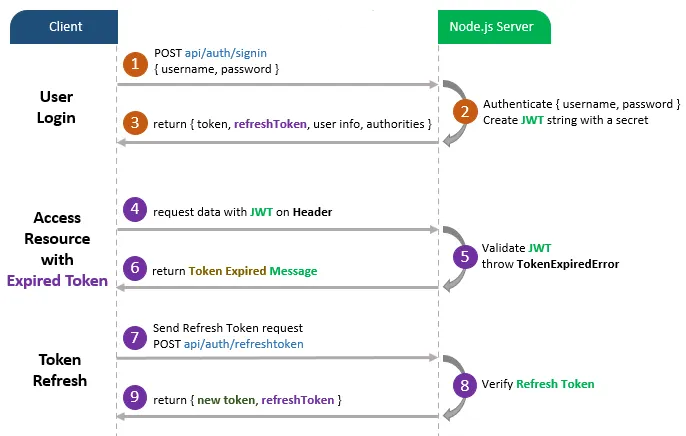
\includegraphics[width=0.85\linewidth]{img/uml/seq_login_token.png}
    \caption{\textit{Biểu đồ Tuần tự Đăng nhập SSO và Phân phối Token Dùng chung}}
    \label{fig:seq_auth_login}
\end{figure}

Biểu đồ hình \ref{fig:seq_auth_login} mô tả chi tiết quy trình người dùng xác thực với máy chủ đăng nhập tập trung, cơ chế phân phối chuỗi JWT dùng chung (\texttt{Shared JWT}) được ký bởi khóa bí mật \texttt{AUTH\_JWT\_SECRET}, cho phép các backend \texttt{hrm-be} và \texttt{ioffice-be} xác thực cục bộ độc lập với độ trễ dưới 5ms. Bên cạnh đó, toàn bộ logic sinh vé, tiêu thụ vé nguyên tử và xử lý lỗi đã được bảo vệ bởi bộ 46 ca kiểm thử tự động (\texttt{sso\_*.unit.test.ts}) đạt tỷ lệ vượt qua 100\%.

\newpage
\subsection{Phân hệ Quản trị Nhân sự (HRM Module)}
\label{subsec:module_hrm}

\subsubsection{Mô tả Nghiệp vụ và Yêu cầu Chức năng}
Phân hệ Quản trị Nhân sự là một trong hai trụ cột nghiệp vụ lớn nhất của ứng dụng di động MyHCMUT, kết nối trực tiếp với dịch vụ nghiệp vụ nhân sự \texttt{hrm-be} và cơ sở dữ liệu \texttt{tcns-dev} của Nhà trường:

\begin{itemize}
    \item \textbf{Quản lý Hồ sơ Lý lịch 11 Danh mục:} Tra cứu toàn diện thông tin cá nhân, đào tạo, ngạch bậc lương, hợp đồng, khen thưởng, kỷ luật, quá trình công tác...; hỗ trợ lưu đệm ngoại tuyến qua SQLite.
    \item \textbf{Đề xuất \& Thẩm định Sửa Lý lịch (Diff Viewer):} Cán bộ gửi đề xuất cập nhật kèm ảnh minh chứng; Chuyên viên Phòng TCCB thẩm định qua giao diện so sánh trực quan sai khác giữa giá trị cũ và giá trị mới trước khi duyệt ghi đè vào hồ sơ chính thức.
    \item \textbf{Đăng ký Nghỉ phép Wizard 4 bước:} Thiết kế Form Wizard 4 bước kết hợp thuật toán kiểm tra ràng buộc thời gian thực 4 tầng từ API \texttt{POST /api/tcns-nghi-phep/validate}:
    \begin{enumerate}
        \item Tính toán chính xác số ngày làm việc thực tế (tự động loại trừ Thứ 7, Chủ nhật và ngày Lễ theo quy định).
        \item Kiểm tra phát hiện trùng lặp lịch nghỉ phép hoặc lịch công tác cá nhân.
        \item Kiểm tra mốc nộp trễ hạn (cảnh báo bắt buộc nhập lý do giải trình nếu nộp trễ quá 3 ngày hoặc 15 ngày tùy loại phép).
        \item Kiểm tra đối soát số dư quỹ phép năm trong bảng \texttt{tcns\_so\_nghi\_phep\_nam}.
    \end{enumerate}
    \item \textbf{Đăng ký \& Phê duyệt Đi công tác (Business Trip):} Cán bộ lập kế hoạch chuyến đi, chọn thành viên đoàn công tác, nhập địa điểm, thời gian, dự toán kinh phí và đính kèm thư mời/kế hoạch PDF; Lãnh đạo Đơn vị và BGH thẩm định phê duyệt đa cấp.
    \item \textbf{Phê duyệt Đơn Hàng loạt (\texttt{AppBatchActionBar}):} Cho phép Lãnh đạo Đơn vị chọn nhiều đơn nghỉ phép hoặc công tác cùng lúc để duyệt hàng loạt chỉ bằng một thao tác, tối ưu hóa thời gian xử lý hành chính.
\end{itemize}

\subsubsection{Đặc tả Ca sử dụng (Use Cases)}

\begin{table}[H]
\centering
\renewcommand{\arraystretch}{1.2}
\small
\begin{tabularx}{\textwidth}{|L{3.2cm}|Y|}
\hline
\textbf{Mã Ca sử dụng} & \textbf{UC\_HRM\_01: Tra cứu \& Thẩm định Chỉnh sửa Lý lịch Cán bộ (Diff Viewer)} \\
\hline
\textbf{Tác nhân} & Cán bộ / Giảng viên (Người gửi), Chuyên viên Phòng TCCB (Người duyệt) \\
\hline
\textbf{Tiền điều kiện} & Cán bộ đã đăng nhập thành công vào ứng dụng MyHCMUT. \\
\hline
\textbf{Hậu điều kiện} & Dữ liệu hồ sơ lý lịch được cập nhật chính thức vào cơ sở dữ liệu nhân sự của Nhà trường. \\
\hline
\textbf{Luồng sự kiện chính} & 
1. Cán bộ mở màn hình \texttt{PersonalProfilePage}, xem 11 danh mục lý lịch chi tiết. \newline
2. Cán bộ chọn trường thông tin cần chỉnh sửa, nhập giá trị mới và đính kèm tệp ảnh minh chứng. \newline
3. Nhấn \textit{``Gửi đề xuất''} $\rightarrow$ Hệ thống ghi nhận vào bảng \texttt{staff\_ly\_lich\_request} ở trạng thái \texttt{PENDING} và phát sự kiện thông báo cho Phòng TCCB. \newline
4. Chuyên viên TCCB mở màn hình \texttt{ApproveProfileDetailPage}, xem thẻ \texttt{ReviewDiffCard} đối chiếu trực quan giá trị cũ (màu đỏ) và giá trị mới (màu xanh lá). \newline
5. Chuyên viên nhấn \textit{``Phê duyệt''} $\rightarrow$ Hệ thống cập nhật dữ liệu mới vào \texttt{staff\_ly\_lich} và gửi thông báo hoàn tất cho Cán bộ. \\
\hline
\textbf{Luồng ngoại lệ} & Nếu Chuyên viên chọn \textit{``Từ chối''}, bắt buộc nhập lý do từ chối $\rightarrow$ Bản ghi chuyển trạng thái \texttt{REJECTED} và thông báo cho Cán bộ biết. \\
\hline
\end{tabularx}
\caption{\textit{Đặc tả Ca sử dụng UC\_HRM\_01: Tra cứu và Thẩm định Sửa Lý lịch}}
\label{tab:uc_hrm_01}
\end{table}

\begin{table}[H]
\centering
\renewcommand{\arraystretch}{1.2}
\small
\begin{tabularx}{\textwidth}{|L{3.2cm}|Y|}
\hline
\textbf{Mã Ca sử dụng} & \textbf{UC\_HRM\_02: Đăng ký Nghỉ phép Form Wizard 4 bước \& Validate Thời gian thực} \\
\hline
\textbf{Tác nhân} & Cán bộ / Giảng viên \\
\hline
\textbf{Tiền điều kiện} & Cán bộ đã đăng nhập; còn tài khoản hoạt động trong hệ thống. \\
\hline
\textbf{Hậu điều kiện} & Đơn nghỉ phép được khởi tạo thành công ở trạng thái \texttt{CHO\_DUYET} và kích hoạt quy trình phê duyệt. \\
\hline
\textbf{Luồng sự kiện chính} & 
1. Cán bộ mở màn hình \texttt{LeaveRequestPage}, bắt đầu Bước 1: Chọn loại nghỉ và lý do nghỉ. \newline
2. Bước 2: Chọn khoảng thời gian (Từ ngày $\rightarrow$ Đến ngày). \newline
3. Hệ thống tự động gọi API \texttt{POST /api/tcns-nghi-phep/validate} để thực thi 4 tầng kiểm tra: (a) Tính số ngày làm việc thực tế, (b) Kiểm tra trùng lịch cá nhân, (c) Kiểm tra mốc nộp trễ hạn, (d) Kiểm tra số dư quỹ phép năm. \newline
4. Nếu vi phạm mốc nộp trễ hạn $\rightarrow$ Bước 3 hiển thị trường bắt buộc nhập lý do giải trình nộp trễ. \newline
5. Bước 4: Cán bộ xác nhận cam kết bàn giao công việc và nhấn nút \textit{``Gửi duyệt''}. \newline
6. Hệ thống lưu bản ghi vào \texttt{tcns\_nghi\_phep\_dang\_ky} và đẩy thông báo tới Lãnh đạo Đơn vị. \\
\hline
\textbf{Luồng ngoại lệ} & Nếu số ngày nghỉ vượt quá số ngày phép còn lại hoặc trùng với lịch công tác đã duyệt $\rightarrow$ Hệ thống cảnh báo đỏ và khóa không cho phép chuyển bước. \\
\hline
\end{tabularx}
\caption{\textit{Đặc tả Ca sử dụng UC\_HRM\_02: Đăng ký Nghỉ phép 4 bước}}
\label{tab:uc_hrm_02}
\end{table}

\begin{table}[H]
\centering
\renewcommand{\arraystretch}{1.2}
\small
\begin{tabularx}{\textwidth}{|L{3.2cm}|Y|}
\hline
\textbf{Mã Ca sử dụng} & \textbf{UC\_HRM\_03: Đăng ký \& Phê duyệt Đi công tác (Business Trip)} \\
\hline
\textbf{Tác nhân} & Cán bộ đăng ký, Lãnh đạo Đơn vị, Ban Giám hiệu / Phòng TCCB \\
\hline
\textbf{Tiền điều kiện} & Cán bộ có kế hoạch đi công tác trong hoặc ngoài nước. \\
\hline
\textbf{Hậu điều kiện} & Chuyến đi công tác được phê duyệt chính thức và cập nhật vào lịch trình công tác. \\
\hline
\textbf{Luồng sự kiện chính} & 
1. Cán bộ mở màn hình \texttt{BusinessTripEditPage}, nhập mục đích, địa điểm, thời gian, phương tiện di chuyển, dự toán kinh phí và chọn danh sách thành viên đoàn. \newline
2. Đính kèm tệp tài liệu PDF (thư mời, kế hoạch công tác) $\rightarrow$ Nhấn \textit{``Gửi duyệt''}. \newline
3. Lãnh đạo Đơn vị nhận thông báo đẩy FCM, mở \texttt{ApproveBtripListPage} xem xét nội dung $\rightarrow$ Nhấn \textit{``Phê duyệt''}. \newline
4. Nếu chuyến công tác yêu cầu cấp trường phê duyệt $\rightarrow$ Hệ thống chuyển tiếp lên Ban Giám hiệu / Phòng TCCB duyệt và cấp số quyết định. \newline
5. Hệ thống chuyển trạng thái \texttt{DA\_DUYET} và thông báo tới toàn bộ thành viên đoàn công tác. \\
\hline
\end{tabularx}
\caption{\textit{Đặc tả Ca sử dụng UC\_HRM\_03: Đăng ký và Phê duyệt Đi công tác}}
\label{tab:uc_hrm_03}
\end{table}

\subsubsection{Biểu đồ Hoạt động (Activity Diagrams)}

\begin{figure}[H]
    \centering
    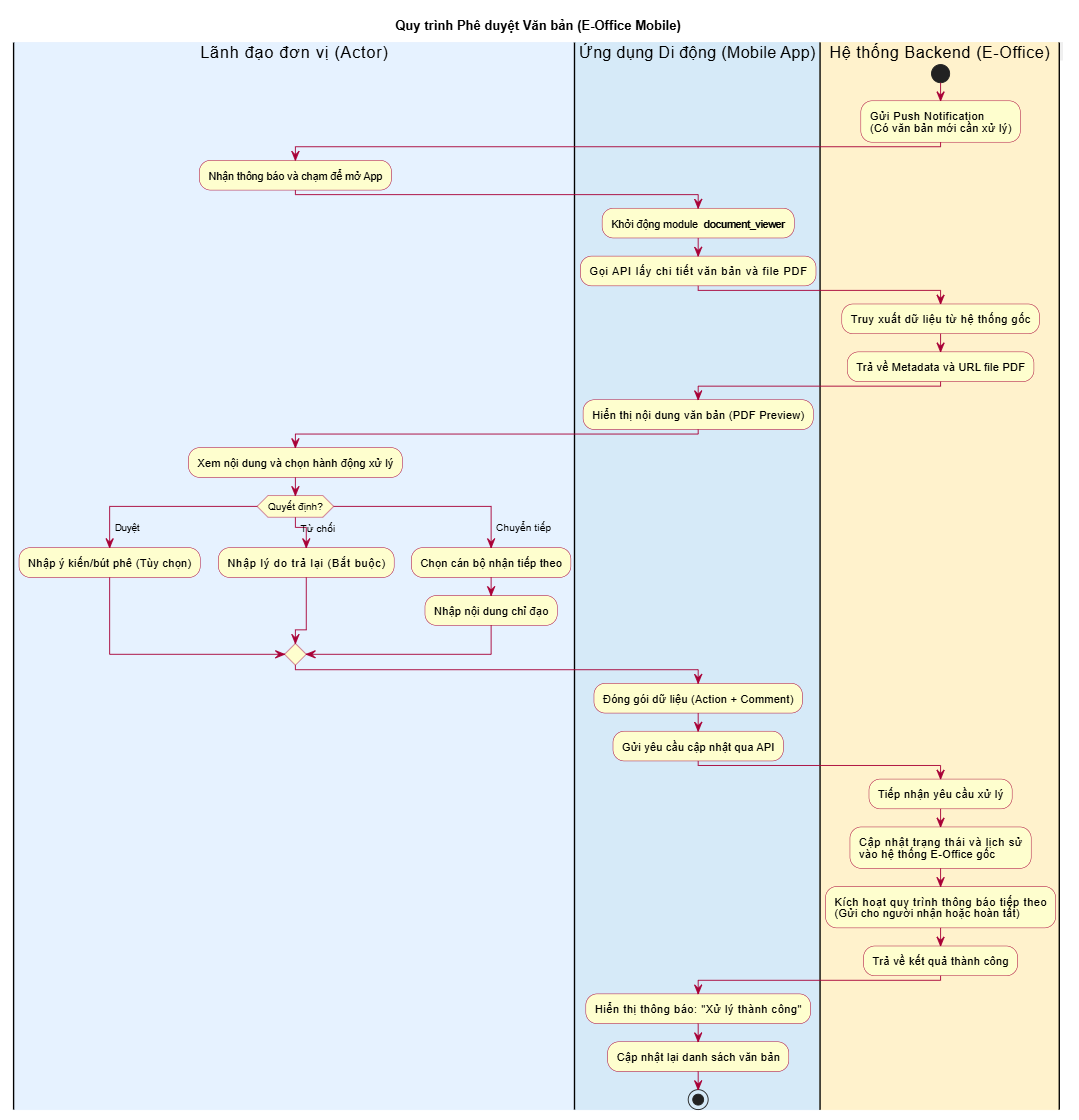
\includegraphics[width=0.85\linewidth]{img/uml/activity_leave_process.png}
    \caption{\textit{Biểu đồ Hoạt động Quy trình Đăng ký và Phê duyệt Nghỉ phép}}
    \label{fig:act_hrm_leave}
\end{figure}

\begin{figure}[H]
    \centering
    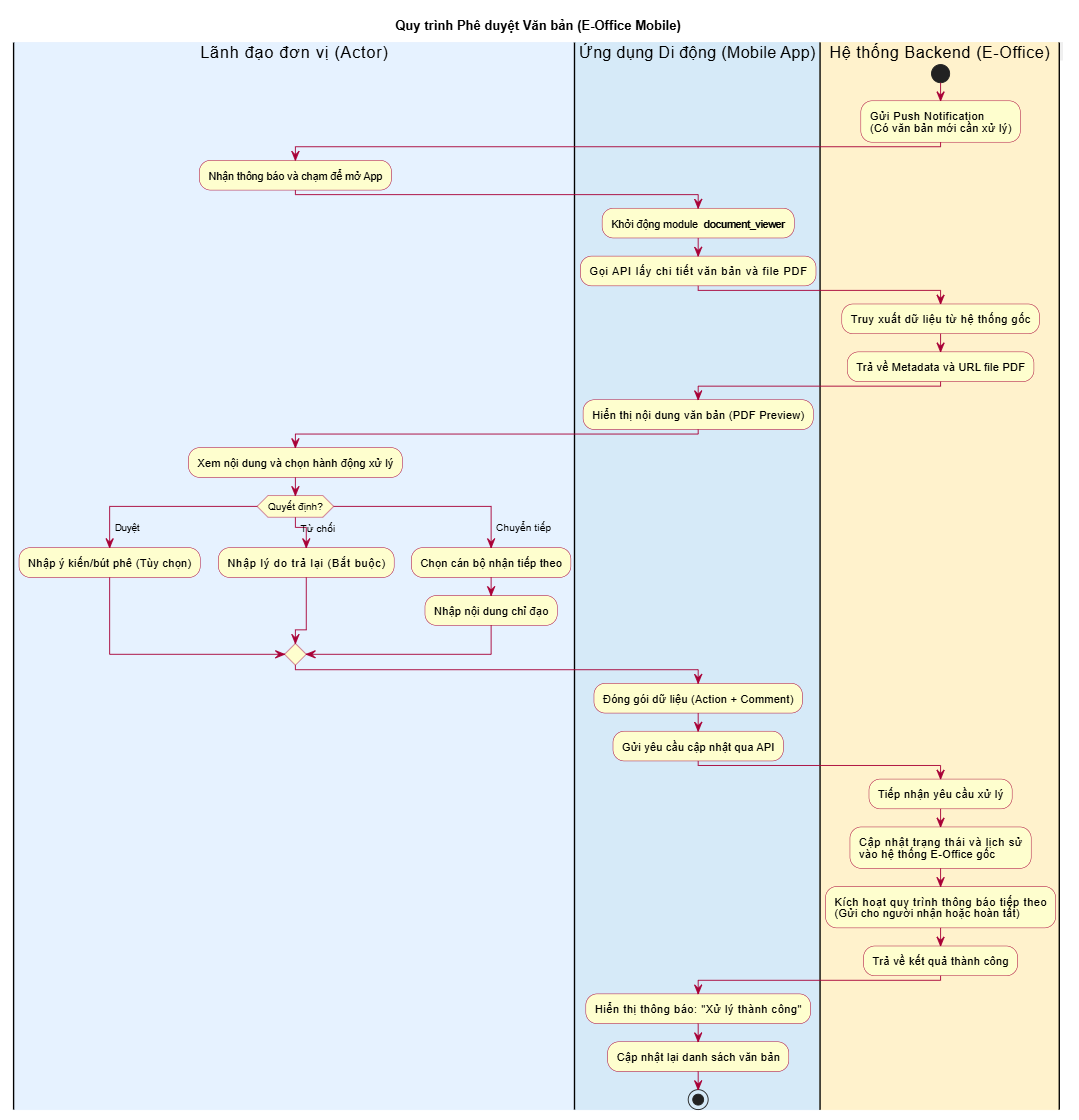
\includegraphics[width=0.85\linewidth]{img/uml/activity_business_trip.png}
    \caption{\textit{Biểu đồ Hoạt động Quy trình Đăng ký và Phê duyệt Đi công tác}}
    \label{fig:act_hrm_btrip}
\end{figure}

\subsubsection{Biểu đồ Tuần tự (Sequence Diagrams)}

\begin{figure}[H]
    \centering
    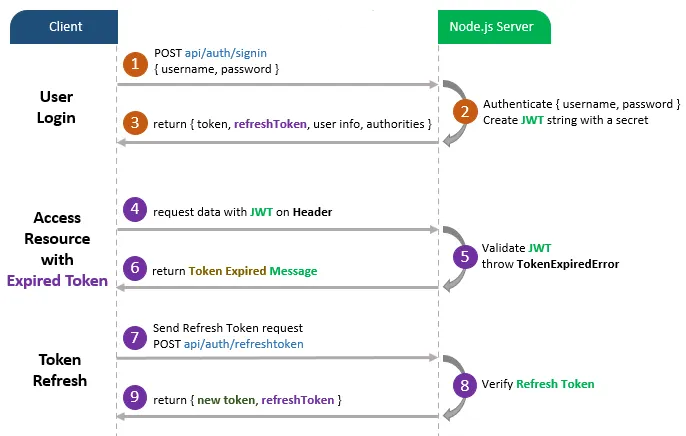
\includegraphics[width=0.85\linewidth]{img/uml/seq_leave_validation.png}
    \caption{\textit{Biểu đồ Tuần tự Đăng ký và Kiểm tra Ràng buộc Nghỉ phép Thời gian thực}}
    \label{fig:seq_hrm_leave_val}
\end{figure}

\begin{figure}[H]
    \centering
    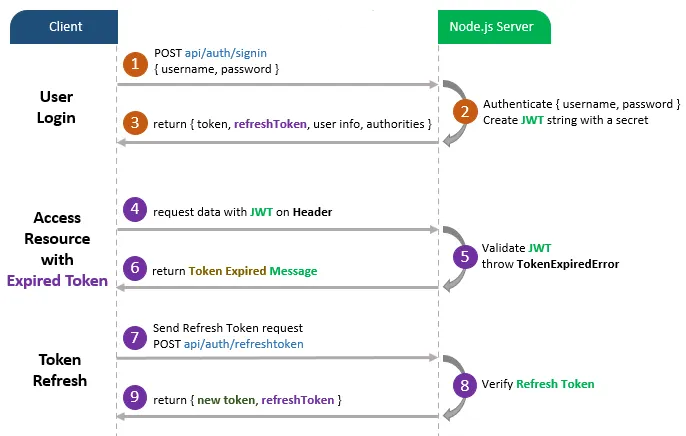
\includegraphics[width=0.85\linewidth]{img/uml/seq_leave_approval.png}
    \caption{\textit{Biểu đồ Tuần tự Phê duyệt Đơn Nghỉ phép Đa cấp}}
    \label{fig:seq_hrm_leave_app}
\end{figure}

\begin{figure}[H]
    \centering
    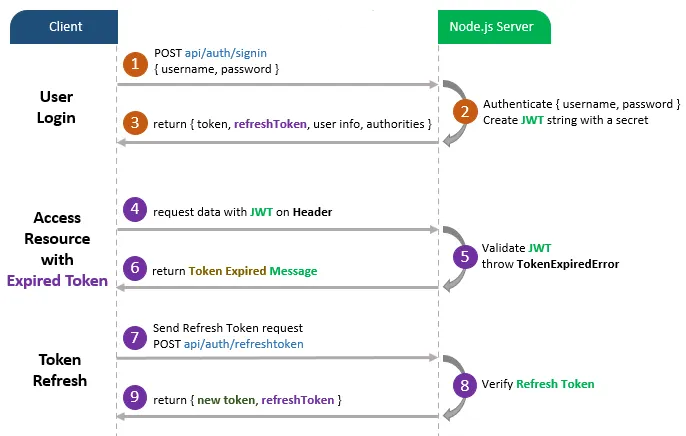
\includegraphics[width=0.85\linewidth]{img/uml/seq_business_trip.png}
    \caption{\textit{Biểu đồ Tuần tự Đăng ký và Phê duyệt Chuyến Đi công tác}}
    \label{fig:seq_hrm_btrip}
\end{figure}

\begin{figure}[H]
    \centering
    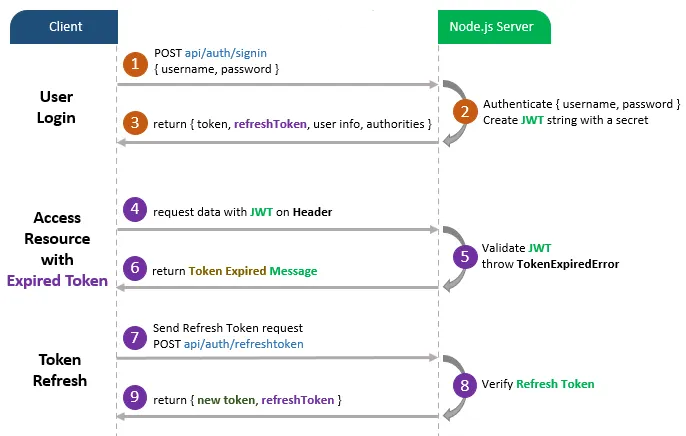
\includegraphics[width=0.85\linewidth]{img/uml/seq_profile_diff.png}
    \caption{\textit{Biểu đồ Tuần tự Thẩm định So sánh Sai khác (Diff Viewer) Sửa Lý lịch}}
    \label{fig:seq_hrm_diff}
\end{figure}

\newpage
\subsection{Phân hệ Văn phòng số, Nhiệm vụ và Lịch công tác (iOffice)}
\label{subsec:module_ioffice}
\label{subsec:req_schedule}

\subsubsection{Mục tiêu}
Phân hệ Văn phòng số, Nhiệm vụ và Lịch công tác kết nối trực tiếp với dịch vụ \texttt{ioffice-be} của Nhà trường, cung cấp cho viên chức, giảng viên khả năng tra cứu văn bản đến/đi, theo dõi tiến độ công việc và chủ động theo dõi các sự kiện lịch công tác tuần của Nhà trường và đơn vị trên thiết bị di động.

Đối với các cuộc họp có cấu hình điểm danh, ứng dụng hỗ trợ tính năng điểm danh có mặt hoặc báo vắng kèm lý do giải trình. Mọi điều kiện hợp lệ về thẩm quyền và khung thời gian điểm danh phải được backend kiểm soát độc lập, không phụ thuộc vào đồng hồ thời gian hoặc trạng thái do thiết bị di động tự thiết lập.

\subsubsection{Yêu cầu chức năng}

\begin{itemize}[leftmargin=1.5cm]
    \item \textbf{FR-SCH-01 -- Xem lịch công tác:} Người dùng có quyền phải có khả năng tra cứu danh sách các sự kiện lịch tuần trường, lịch đơn vị và xem thông tin chi tiết: chủ trì, thời gian bắt đầu/kết thúc, địa điểm, thành phần tham dự và nội dung cuộc họp.
    
    \item \textbf{FR-SCH-02 -- Hiển thị thao tác điểm danh:} Đối với các cuộc họp có cấu hình điểm danh, ứng dụng phải tự động hiển thị nút bấm thao tác điểm danh/báo vắng khi sự kiện nằm trong khoảng thời gian cho phép.
    
    \item \textbf{FR-SCH-03 -- Điểm danh có mặt:} Người dùng phải có khả năng gửi yêu cầu ghi nhận có mặt đối với cuộc họp mà mình có tên trong danh sách đại biểu được mời tham dự.
    
    \item \textbf{FR-SCH-04 -- Báo vắng:} Người dùng có thể khai báo vắng mặt và bắt buộc phải cung cấp lý do vắng hợp lệ (độ dài quy định) khi chức năng này được sự kiện cho phép.
    
    \item \textbf{FR-SCH-05 -- Kiểm tra tại backend:} Backend phải thẩm định lại danh tính người dùng, quyền tham dự cuộc họp và điều kiện khung giờ hợp lệ trước khi ghi nhận trạng thái điểm danh vào cơ sở dữ liệu.
    
    \item \textbf{FR-SCH-06 -- Đồng bộ thay đổi:} Khi trạng thái điểm danh của cuộc họp thay đổi, ứng dụng phải cập nhật ngay giao diện hiển thị; các thay đổi phát sinh từ người dùng khác có thể được cập nhật theo thời gian thực qua kênh kết nối mạng của hệ thống.
\end{itemize}

\subsubsection{Đặc tả Ca sử dụng (Use Cases)}

\usecasespec{
  id={UC-SCH-01},
  name={Điểm danh cuộc họp},
  actor={Cán bộ / Giảng viên có tên trong danh sách tham dự cuộc họp.},
  pre={Người dùng đã đăng nhập; cuộc họp được cấu hình hỗ trợ ghi nhận tham dự.},
  trigger={Người dùng mở xem chi tiết cuộc họp trên ứng dụng.},
  mainflow={
    1. Mobile kiểm tra sơ bộ khung giờ diễn ra cuộc họp và hiển thị các tùy chọn điểm danh. \newline
    2. Người dùng nhấn nút \textit{``Điểm danh có mặt''} (hoặc \textit{``Báo vắng''} kèm nhập lý do). \newline
    3. Mobile gửi request lên backend dịch vụ. \newline
    4. Backend kiểm tra tính hợp lệ của phiên, quyền tham dự của cán bộ và thời gian hiện tại trên máy chủ. \newline
    5. Backend ghi nhận trạng thái tham dự vào cơ sở dữ liệu và phát sự kiện đồng bộ. \newline
    6. Mobile nhận phản hồi thành công và cập nhật trạng thái hiển thị trên giao diện sang \textit{``Đã điểm danh''}.
  },
  altflow={
    Cuộc họp chưa đến giờ mở điểm danh, đã kết thúc hoặc cán bộ không thuộc danh sách tham dự $\rightarrow$ Backend từ chối ghi nhận; ứng dụng hiển thị thông báo lỗi tương ứng.
  },
  post={Bản ghi tham dự cuộc họp của cán bộ được lưu trữ chính thức tại hệ thống iOffice.},
  label={tab:uc_sch_01}
}

\usecasespec{
  id={UC-IOFFICE-01},
  name={Tra cứu Văn bản Đến/Đi và Bút phê Phân phối Chỉ đạo},
  actor={Cán bộ xem văn bản, Lãnh đạo Đơn vị (Người chỉ đạo)},
  pre={Cán bộ đã đăng nhập; có quyền truy cập văn phòng điện tử.},
  mainflow={
    1. Cán bộ mở màn hình \texttt{IncomingDocsListPage} hoặc \texttt{OutgoingDocsListPage}. \newline
    2. Hệ thống tải danh sách văn bản phân trang cuộn vô tận (\texttt{InfiniteScrollPagination}). \newline
    3. Nhấn vào một văn bản cụ thể $\rightarrow$ Mở màn hình \texttt{IncomingDocDetailPage}, tích hợp trình đọc PDF (\texttt{pdfrx}) hiển thị nội dung toàn văn. \newline
    4. Lãnh đạo Đơn vị nhấn nút \textit{``Phân phối văn bản''}, chọn cán bộ xử lý chính, cán bộ phối hợp, hạn chót và nhập bút phê chỉ đạo. \newline
    5. Nhấn \textit{``Lưu chỉ đạo''} $\rightarrow$ Hệ thống ghi nhận vào \texttt{van\_ban\_den\_distribution} và phát thông báo đẩy tới các cán bộ được giao việc.
  },
  post={Cán bộ đọc được nội dung văn bản; văn bản được phân phối kèm chỉ đạo xử lý.},
  label={tab:uc_ioffice_01}
}

\usecasespec{
  id={UC-IOFFICE-02},
  name={Quản lý \& Giám sát Tiến độ Nhiệm vụ (Tasks/Missions)},
  actor={Cán bộ thực hiện, Lãnh đạo Đơn vị, Ban Giám hiệu},
  pre={Nhiệm vụ đã được khởi tạo trong hệ thống điều hành của Nhà trường.},
  mainflow={
    1. Người dùng mở \texttt{MissionsListPage}, lọc theo loại nhiệm vụ (Trọng tâm/Được giao/Chung) và 5 trạng thái. \newline
    2. Chọn một nhiệm vụ cụ thể $\rightarrow$ Mở \texttt{MissionDetailPage} với 4 tab (Tổng quan, Cây đầu việc \texttt{outlined-tree}, Báo cáo đợt, Văn bản liên kết). \newline
    3. Nhấn vào một công việc trong cây đầu việc $\rightarrow$ Mở \texttt{TaskDetailBottomSheet} để xem người phụ trách và checklist. \newline
    4. Cán bộ nhấn \textit{``Nộp báo cáo đợt''}, nhập nội dung, \% tiến độ hoàn thành và đính kèm tài liệu minh chứng $\rightarrow$ Nhấn gửi. \newline
    5. Hệ thống lưu vào bảng \texttt{mission\_report\_batch} và cập nhật lại tiến độ tổng thể của nhiệm vụ.
  },
  post={Cán bộ cập nhật tiến độ công việc và gửi báo cáo đợt thành công.},
  label={tab:uc_ioffice_02}
}

\subsubsection{Quy tắc nghiệp vụ (Business Rules)}

\begin{itemize}[leftmargin=1.5cm]
    \item \textbf{BR-SCH-01:} Chỉ các sự kiện lịch họp được nhà trường cấu hình bật tính năng ghi nhận tham dự mới cho phép người dùng thực hiện điểm danh hoặc báo vắng.
    \item \textbf{BR-SCH-02:} Điều kiện thời gian kiểm tra trên thiết bị di động chỉ đóng vai trò hỗ trợ giao diện (UX Gate); thời gian trên máy chủ backend (Server Time) là căn cứ thẩm quyền duy nhất để quyết định tính hợp lệ của thao tác điểm danh.
    \item \textbf{BR-SCH-03:} Người dùng chỉ được phép điểm danh cho các cuộc họp mà tài khoản của họ được phân công tham dự hoặc được mời với tư cách đại biểu hợp lệ.
    \item \textbf{BR-SCH-04:} Khi thực hiện báo vắng, nội dung lý do báo vắng bắt buộc phải thỏa mãn yêu cầu về độ dài và định dạng do backend quy định (ví dụ tối thiểu từ 1 đến 200 ký tự).
    \item \textbf{BR-SCH-05:} Ứng dụng di động không được xem dữ liệu nhận được từ kênh thời gian thực (real-time stream) là nguồn dữ liệu có thẩm quyền thay thế cho trạng thái lưu trữ chính thức trong cơ sở dữ liệu backend.
\end{itemize}

\subsubsection{Biểu đồ Hoạt động (Activity Diagrams)}

\begin{figure}[H]
    \centering
    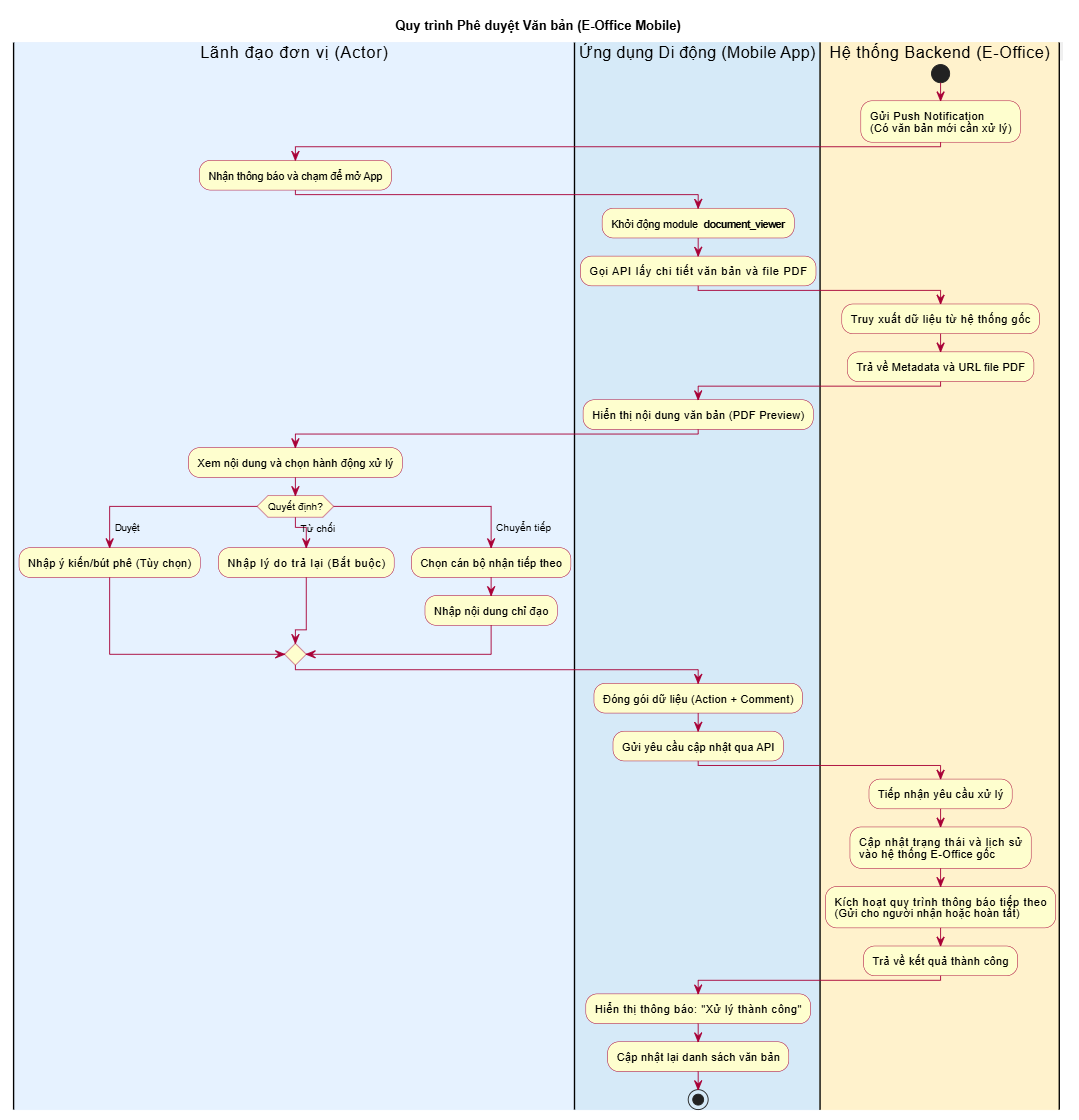
\includegraphics[width=0.85\linewidth]{img/uml/activity_mission_workflow.png}
    \caption{\textit{Biểu đồ Hoạt động Quy trình Quản lý và Theo dõi Tiến độ Nhiệm vụ}}
    \label{fig:act_ioffice_mission}
\end{figure}

\begin{figure}[H]
    \centering
    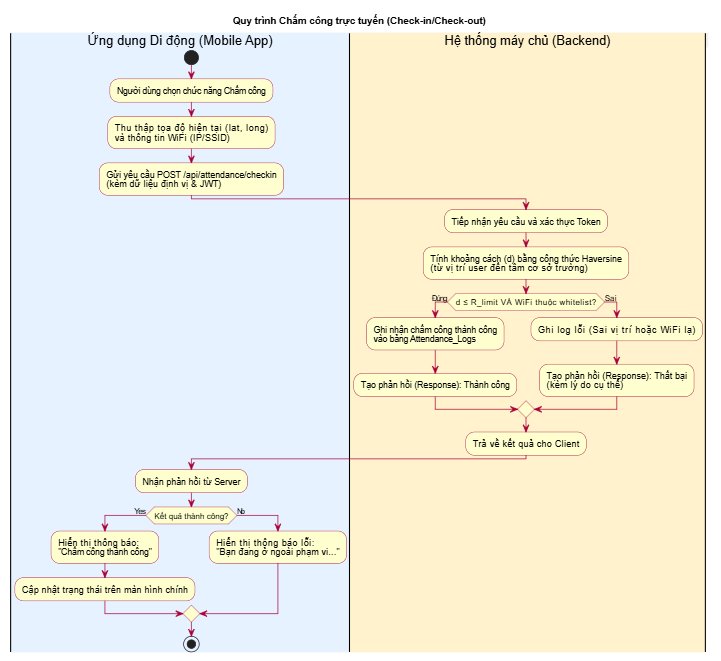
\includegraphics[width=0.85\linewidth]{img/uml/activity_schedule_attendance.png}
    \caption{\textit{Biểu đồ Hoạt động Quy trình Điểm danh Cuộc họp Thời gian thực}}
    \label{fig:act_ioffice_attendance}
\end{figure}

\subsubsection{Biểu đồ Tuần tự (Sequence Diagrams)}

\begin{figure}[H]
    \centering
    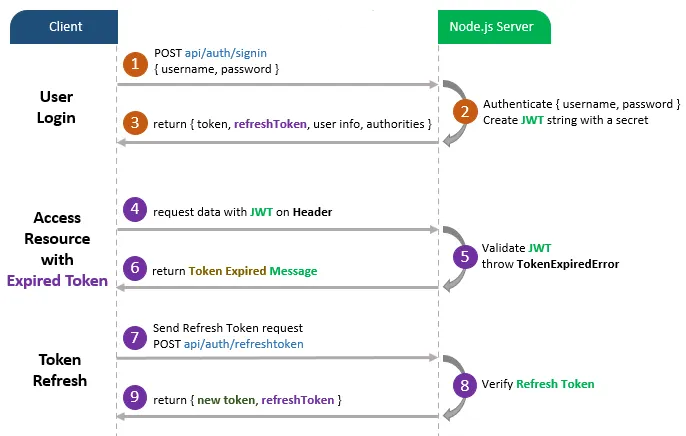
\includegraphics[width=0.85\linewidth]{img/uml/seq_mission_tasks.png}
    \caption{\textit{Biểu đồ Tuần tự Quản lý Nhiệm vụ, Cây Đầu việc và Báo cáo Tiến độ}}
    \label{fig:seq_ioffice_mission}
\end{figure}

\begin{figure}[H]
    \centering
    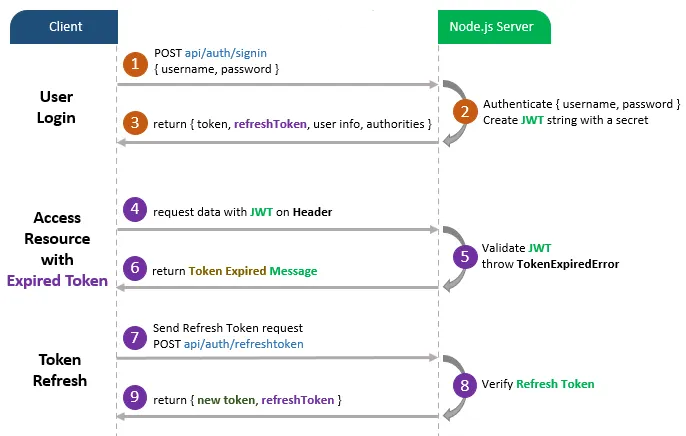
\includegraphics[width=0.85\linewidth]{img/uml/seq_meeting_checkin.png}
    \caption{\textit{Biểu đồ Tuần tự Điểm danh Cuộc họp Thời gian thực qua WebSocket Socket.IO}}
    \label{fig:seq_ioffice_checkin}
\end{figure}

\newpage
\subsection{Phân hệ Thông báo}
\label{subsec:req_notification}
\label{subsec:module_notification}

\subsubsection{Mục tiêu}
Phân hệ Thông báo cung cấp một điểm tiếp nhận thông tin và sự kiện nghiệp vụ tập trung trên ứng dụng di động cho toàn bộ các dịch vụ HRM và iOffice.

Mục tiêu của phân hệ không chỉ dừng lại ở việc hiển thị các biểu ngữ (banner) thông báo đẩy tức thời, mà còn hỗ trợ người dùng nhận diện ngữ cảnh nghiệp vụ và kích hoạt cơ chế điều hướng sâu (Deep Linking) trực tiếp đến đúng màn hình đối tượng cần xử lý trên ứng dụng.

\subsubsection{Yêu cầu chức năng}

\begin{itemize}[leftmargin=1.5cm]
    \item \textbf{FR-NOT-01 -- Đăng ký thiết bị nhận thông báo:} Sau khi người dùng đăng nhập thành công và thiết bị được cấp FCM Device Token từ dịch vụ Firebase, ứng dụng Mobile phải tự động gửi token này lên backend để liên kết với tài khoản người dùng hiện tại.
    
    \item \textbf{FR-NOT-02 -- Cập nhật token:} Khi dịch vụ FCM làm mới hoặc cấp lại token cho thiết bị, ứng dụng phải tự động phát hiện và gửi token mới lên backend để cập nhật thông tin tiếp nhận.
    
    \item \textbf{FR-NOT-03 -- Nhận thông báo:} Ứng dụng phải hỗ trợ tiếp nhận thông báo đẩy trong mọi trạng thái hoạt động của thiết bị (Foreground, Background, Terminated) phù hợp với cơ chế của hệ điều hành Android và iOS.
    
    \item \textbf{FR-NOT-04 -- Xem trung tâm thông báo:} Người dùng có thể mở Trung tâm thông báo trên ứng dụng để xem danh sách toàn bộ các thông báo đã nhận, phân biệt rõ ràng giữa thông báo đã đọc và chưa đọc.
    
    \item \textbf{FR-NOT-05 -- Cập nhật trạng thái đọc:} Khi người dùng mở xem thông báo hoặc thực hiện thao tác đánh dấu đã đọc, hệ thống phải cập nhật trạng thái tương ứng trên giao diện và gửi request đồng bộ về backend.
    
    \item \textbf{FR-NOT-06 -- Điều hướng theo ngữ cảnh (Deep Linking):} Khi người dùng chạm vào một thông báo có dữ liệu định tuyến hợp lệ, ứng dụng phải trích xuất các trường thông tin chuẩn hóa để xác định chính xác màn hình cần mở:
\end{itemize}

\begin{table}[H]
\centering
\renewcommand{\arraystretch}{1.25}
\begin{tabularx}{\textwidth}{|p{3.5cm}|X|}
\hline
\textbf{Trường Metadata} & \textbf{Ý nghĩa nghiệp vụ phục vụ định tuyến} \\
\hline
\texttt{source} & Miền dịch vụ phát sinh thông báo (ví dụ \texttt{'hrm'} hoặc \texttt{'ioffice'}). \\
\hline
\texttt{entityType} & Loại đối tượng nghiệp vụ (\texttt{'leave'}, \texttt{'business-trip'}, \texttt{'incoming-doc'}, \texttt{'outgoing-doc'}, \texttt{'task'}). \\
\hline
\texttt{entityId} & Khóa chính định danh duy nhất của bản ghi đối tượng cần mở (ID đơn nghỉ phép, ID nhiệm vụ...). \\
\hline
\texttt{isApproval} & Cờ đánh dấu ngữ cảnh: \texttt{true} nếu cần mở giao diện phê duyệt của cấp quản lý, \texttt{false} nếu mở giao diện xem chi tiết thông thường. \\
\hline
\end{tabularx}
\caption{\textit{Chuẩn hóa các trường Metadata định tuyến thông báo}}
\label{tab:notification_metadata}
\end{table}

\begin{itemize}[leftmargin=1.5cm]
    \item \textbf{FR-NOT-07 -- Xử lý thông báo không còn hợp lệ:} Trường hợp đối tượng được thông báo tham chiếu đã bị xóa, người dùng không còn quyền truy cập hoặc route điều hướng không xác định được, ứng dụng tuyệt đối không được điều hướng tới một màn hình sai hoặc làm dừng đột ngột ứng dụng; hệ thống phải hiển thị thông báo giải thích nhẹ nhàng và giữ người dùng ở trạng thái an toàn.
    
    \item \textbf{FR-NOT-08 -- Đăng xuất thiết bị:} Khi người dùng đăng xuất, ứng dụng phải gửi request yêu cầu backend hủy liên kết giữa FCM token của thiết bị và tài khoản người dùng, nhằm ngăn chặn triệt để nguy cơ gửi thông báo nghiệp vụ của người dùng cũ đến thiết bị.
\end{itemize}

\subsubsection{Đặc tả Ca sử dụng (Use Cases)}

\usecasespec{
  id={UC-NOT-01},
  name={Xem và mở thông báo},
  actor={Người dùng ứng dụng MyHCMUT Mobile.},
  pre={Người dùng đã đăng nhập vào ứng dụng.},
  trigger={Người dùng mở Trung tâm thông báo hoặc chạm vào thông báo đẩy xuất hiện trên màn hình khóa / thanh trạng thái.},
  mainflow={
    1. Hệ thống lấy danh sách thông báo và hiển thị trạng thái đã đọc/chưa đọc. \newline
    2. Người dùng chọn một mục thông báo cụ thể. \newline
    3. Ứng dụng đánh dấu thông báo là đã đọc và phân tích 4 trường metadata (\texttt{source}, \texttt{entityType}, \texttt{entityId}, \texttt{isApproval}). \newline
    4. Hệ thống xác định đường dẫn điều hướng (Route) tương ứng và kích hoạt chuyển màn hình trực tiếp đến đúng đối tượng nghiệp vụ.
  },
  altflow={
    Metadata không hợp lệ hoặc bản ghi đối tượng đã bị xóa $\rightarrow$ Hệ thống hiển thị thông báo đối tượng không khả dụng và không thực hiện điều hướng sai.
  },
  post={Người dùng được đưa tới đúng ngữ cảnh cần thao tác; trạng thái thông báo được cập nhật là Đã đọc.},
  label={tab:uc_not_01}
}

\usecasespec{
  id={UC-NOT-02},
  name={Quản lý token thiết bị},
  actor={Ứng dụng Mobile (thực thi tự động dưới nền).},
  trigger={Người dùng đăng nhập thành công, FCM token được làm mới, hoặc người dùng đăng xuất.},
  mainflow={
    1. Ứng dụng nhận FCM Device Token từ dịch vụ Google Firebase. \newline
    2. Gửi request kèm token và định danh người dùng lên backend dịch vụ thông báo. \newline
    3. Backend kiểm tra và cập nhật bản ghi ánh xạ giữa \texttt{user\_id} và \texttt{device\_token} trong bảng dữ liệu thiết bị. \newline
    4. Khi người dùng đăng xuất, ứng dụng gửi lệnh thu hồi để backend hủy kích hoạt token tương ứng.
  },
  post={Cơ sở dữ liệu backend duy trì danh sách các token thiết bị đang hoạt động hợp lệ cho người dùng.},
  label={tab:uc_not_02}
}

\subsubsection{Quy tắc nghiệp vụ (Business Rules)}

\begin{itemize}[leftmargin=1.5cm]
    \item \textbf{BR-NOT-01:} Người dùng chỉ được phép truy xuất và thao tác trên danh sách các thông báo thuộc quyền sở hữu của chính tài khoản mình.
    \item \textbf{BR-NOT-02:} Toàn bộ dữ liệu metadata điều hướng gửi kèm thông báo phải được kiểm tra và chuẩn hóa trước khi tạo lệnh điều hướng; ứng dụng không được tin cậy hoàn toàn dữ liệu push như một lệnh điều hướng tự do.
    \item \textbf{BR-NOT-03:} Các tham số \texttt{source}, \texttt{entityType}, \texttt{entityId} và ngữ cảnh \texttt{isApproval} bắt buộc phải được ánh xạ sang các route nội bộ đã được định nghĩa tĩnh trong bộ định tuyến của ứng dụng.
    \item \textbf{BR-NOT-04:} Quyền truy cập vào đối tượng nghiệp vụ sau khi điều hướng sâu (Deep Link) vẫn phải được backend kiểm tra độc lập; việc nhận được thông báo không đồng nghĩa với việc tự động được cấp quyền thao tác.
    \item \textbf{BR-NOT-05:} FCM Device Token có thể thay đổi trong suốt vòng đời của ứng dụng; Mobile phải cài đặt cơ chế lắng nghe sự kiện làm mới token để kịp thời cập nhật lên máy chủ.
    \item \textbf{BR-NOT-06:} Khi dịch vụ Firebase FCM phản hồi thông báo về một token không còn hợp lệ (Unregistered / Invalid Token), backend phải tự động xóa hoặc gắn cờ vô hiệu hóa token đó trong cơ sở dữ liệu.
    \item \textbf{BR-NOT-07:} Tính năng hiển thị số đếm huy hiệu (Badge Counter) phụ thuộc hoàn toàn vào hệ điều hành và giao diện trình khởi chạy (Launcher) của từng dòng máy; hệ thống không cam kết mọi thiết bị đều hiển thị số badge đồng nhất.
    \item \textbf{BR-NOT-08:} Hệ thống không giả định rằng mọi sự kiện thông báo đẩy đều được phân phối tới thiết bị chính xác một lần (không bảo đảm Exactly-Once). Phân hệ thông báo chỉ đóng vai trò kênh hỗ trợ thông tin nhanh; trạng thái nghiệp vụ chuẩn mực cuối cùng luôn phải được truy vấn từ backend.
\end{itemize}

\subsubsection{Biểu đồ Tuần tự (Sequence Diagrams)}

\begin{figure}[H]
    \centering
    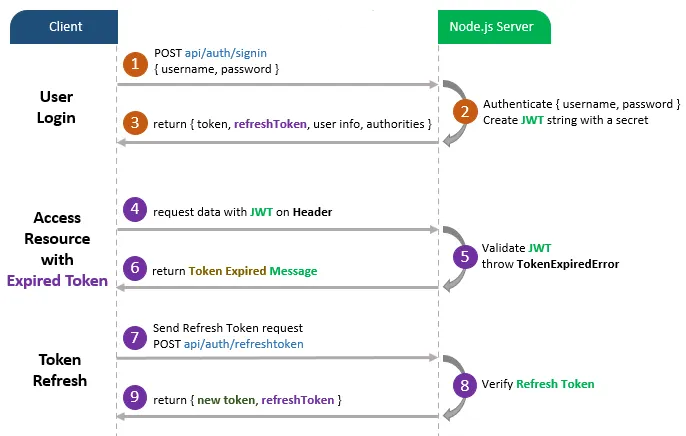
\includegraphics[width=0.85\linewidth]{img/uml/seq_kafka_fcm_push.png}
    \caption{\textit{Biểu đồ Tuần tự Pipeline Thông báo Đẩy Bất đồng bộ (Kafka sang FCM sang Mobile)}}
    \label{fig:seq_noti_kafka_fcm}
\end{figure}

Biểu đồ hình \ref{fig:seq_noti_kafka_fcm} thể hiện toàn bộ quy trình phát tán thông báo bất đồng bộ. Điểm mấu chốt trong thiết kế là việc tách biệt ranh giới giao dịch cơ sở dữ liệu với việc phát thông điệp vào Kafka: hàm phát tán chỉ được gọi sau khi lệnh \texttt{transaction.commit()} đã hoàn tất thành công. Nhờ đó, hệ thống ngăn chặn hoàn toàn hiện tượng người dùng nhận thông báo về một đơn từ hoặc quyết định đã bị hủy bỏ do lỗi giao dịch ở tầng cơ sở dữ liệu. Toàn bộ logic giải mã metadata và điều hướng sâu đã được kiểm thử tự động với 47 ca kiểm thử chuyên biệt cho module thông báo.

\newpage
\subsection{Phân hệ Khoa học Công nghệ (KHCN Module -- Phân hệ Mở rộng)}
\label{subsec:module_khcn}

\subsubsection{Mô tả Nghiệp vụ và Định hướng Tích hợp}
Phân hệ Khoa học Công nghệ (tương ứng với gói mã nguồn \texttt{modules/khcn}) được nhóm thiết kế sẵn về mặt giao diện người dùng (UI Mock \& Component Templates) nhằm phục vụ chiến lược mở rộng chuyển đổi số toàn diện của Trường Đại học Bách khoa:

\begin{itemize}
    \item \textbf{Kê khai Hoạt động NCKH:} Cung cấp form giao diện tra cứu và đăng ký danh mục các đề tài nghiên cứu khoa học các cấp (Cấp Trường, Cấp ĐHQG, Cấp Bộ, Cấp Nhà nước).
    \item \textbf{Kê khai Công bố Khoa học:} Hỗ trợ cán bộ cập nhật danh mục bài báo khoa học đã xuất bản (Tạp chí ISI/Scopus, Kỷ yếu hội nghị quốc tế, Tạp chí trong nước).
    \item \textbf{Theo dõi Khen thưởng \& Sở hữu Trí tuệ:} Tra cứu thông tin bằng sáng chế, giải pháp hữu ích và các quyết định khen thưởng thành tích nghiên cứu.
\end{itemize}

\subsubsection{Đặc tả Phạm vi Hiện thực}
Trong phạm vi hiện tại của đồ án tốt nghiệp, do phía Phòng Khoa học Công nghệ của Nhà trường đang trong quá trình nâng cấp và chuẩn hóa hệ thống Backend RESTful API, phân hệ này được nhóm hiện thực hóa ở mức độ hoàn thiện kiến trúc giao diện người dùng (UI Components \& Route Registration), sẵn sàng kết nối dữ liệu chính thức ngay khi hệ thống Backend của Nhà trường cung cấp cổng API mở.


\newpage
\section{Yêu cầu Phi chức năng và Ràng buộc Kỹ thuật}
\label{sec:yeucau_phichucnang}

Để đảm bảo trải nghiệm sử dụng tin cậy, an toàn và mượt mà cho đội ngũ cán bộ, giảng viên, ứng dụng MyHCMUT phải đáp ứng các tiêu chuẩn yêu cầu phi chức năng nghiêm ngặt:

\begin{itemize}
    \item \textbf{Hiệu năng và Độ mượt mà (Rendering Performance):}
    \begin{itemize}
        \item Tốc độ khung hình (Frame Rate) duy trì ổn định trong khoảng **58--60 FPS** khi cuộn các danh sách dữ liệu lớn (danh sách văn bản, danh sách công việc).
        \item Thời gian khởi động ứng dụng ở trạng thái nguội (Cold Start) $< 1.5$ giây; khởi động nóng (Warm Start) $< 0.5$ giây.
        \item Thời gian phản hồi trung bình của các API Endpoints cốt lõi $< 150$ms.
    \end{itemize}
    
    \item \textbf{Độ trễ Thông báo Đẩy (Notification Latency):}
    \begin{itemize}
        \item Tổng độ trễ truyền phát thông điệp đầu-cuối từ khi sự kiện nghiệp vụ phát sinh trên Backend, luân chuyển qua Kafka broker, chuyển tiếp tới Google FCM Server và hiển thị lên thiết bị di động của người dùng đạt mức $\approx 1.0$ giây (luôn duy trì dưới $2.0$ giây).
    \end{itemize}

    \item \textbf{Bảo mật và Quyền riêng tư (Security \& Privacy):}
    \begin{itemize}
        \item Toàn bộ các kết nối giao tiếp mạng giữa ứng dụng di động và máy chủ đều bắt buộc mã hóa qua giao thức an toàn HTTPS/TLS.
        \item Mã hóa cặp khóa xác thực Access Token và Refresh Token trong không gian lưu trữ an toàn của hệ điều hành.
        \item Kiểm soát phân quyền đa tầng (RBAC) nghiêm ngặt tại cả tầng giao diện (Route Guards trên Mobile) và tầng dịch vụ (Middleware trên Backend).
    \end{itemize}

    \item \textbf{Độ tin cậy và Khả năng Chịu lỗi (Reliability \& Fault-Tolerance):}
    \begin{itemize}
        \item Khi xảy ra sự cố mất kết nối mạng hoặc lỗi máy chủ (Timeout), ứng dụng bắt lỗi tập trung và thông báo nhẹ nhàng qua giao diện thông báo (Snackbar / Toast), cung cấp nút Thử lại (Retry), tuyệt đối không làm ứng dụng bị dừng đột ngột (Crash).
        \item Tự động làm mới phiên làm việc ngầm (Silent Refresh) khi Access Token hết hạn, đảm bảo trải nghiệm liền mạch cho người dùng.
    \end{itemize}

    \item \textbf{Tối ưu hóa Tài nguyên Phần cứng (Resource Consumption):}
    \begin{itemize}
        \item Mức tiêu thụ bộ nhớ RAM ở trạng thái tĩnh duy trì dưới 100 MB; khi tải dữ liệu tối đa và xem tài liệu PDF lớn không vượt quá 150 MB.
        \item Kích thước tệp cài đặt ứng dụng (APK Release) tối ưu dưới 30 MB nhờ cơ chế nén tài nguyên và phân tách kiến trúc ABI.
    \end{itemize}
\end{itemize}

%%% CHUONG 5: PHAN TICH VA THIET KE HE THONG
\newpage
\chapter{ĐẶC TẢ CHI TIẾT CÁC USE-CASE VÀ BIỂU ĐỒ HOẠT ĐỘNG}
\label{chap:dacta_usecase}

Trong chương này, nhóm trình bày Sơ đồ Ca sử dụng tổng thể toàn hệ thống, các Bảng đặc tả chi tiết 5 Use Cases cốt lõi, cùng hệ thống Biểu đồ hoạt động (Activity Diagrams) và Biểu đồ tuần tự (Sequence Diagrams) mô tả chi tiết các quy trình nghiệp vụ và luồng tương tác của ứng dụng MyHCMUT.

\newpage
\section{Sơ đồ Ca sử dụng Tổng thể Toàn hệ thống}
\label{sec:system_usecase}

\begin{figure}[H]
    \centering
    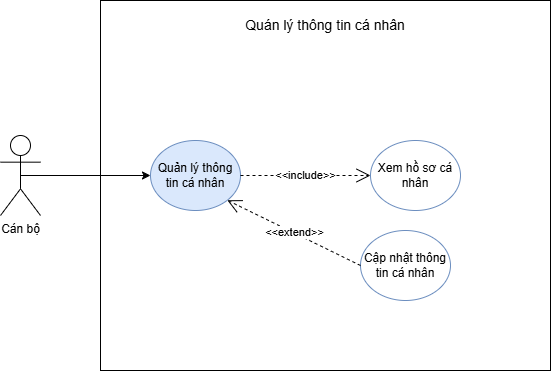
\includegraphics[width=0.9\linewidth]{img/uml/system_usecase_diagram.png}
    \caption{\textit{Sơ đồ Ca sử dụng Tổng thể Hệ thống MyHCMUT}}
    \label{fig:usecase_overall}
\end{figure}

\section{Bảng Đặc tả Chi tiết các Ca sử dụng Cốt lõi}
\label{sec:dacta_usecase_chitiet}

\subsection{UC01: Tra cứu \& Đề xuất Thẩm định Chỉnh sửa Lý lịch Cán bộ}
\begin{table}[H]
\centering
\renewcommand{\arraystretch}{1.2}
\begin{tabularx}{\textwidth}{|p{3.2cm}|X|}
\hline
\textbf{Tên Ca sử dụng} & \textbf{UC01: Tra cứu \& Đề xuất Thẩm định Chỉnh sửa Lý lịch Cán bộ} \\
\hline
\textbf{Tác nhân} & Cán bộ/Giảng viên (Người gửi), Chuyên viên Phòng TCCB (Người duyệt) \\
\hline
\textbf{Tiền điều kiện} & Cán bộ đã đăng nhập thành công vào ứng dụng MyHCMUT. \\
\hline
\textbf{Hậu điều kiện} & Dữ liệu hồ sơ lý lịch được cập nhật chính thức vào cơ sở dữ liệu nhân sự. \\
\hline
\textbf{Luồng sự kiện chính} & 
1. Cán bộ mở màn hình \texttt{PersonalProfilePage}, xem 11 tab lý lịch chi tiết. \newline
2. Cán bộ chọn mục cần chỉnh sửa, nhập giá trị mới và đính kèm ảnh minh chứng. \newline
3. Nhấn nút \textit{``Gửi đề xuất''} $\rightarrow$ Hệ thống lưu vào bảng \texttt{staff\_ly\_lich\_request} (trạng thái \texttt{PENDING}) và đẩy thông báo cho Phòng TCCB. \newline
4. Chuyên viên TCCB mở màn hình \texttt{ApproveProfileDetailPage}, xem giao diện Diff Viewer so sánh trực quan giá trị cũ (màu đỏ) và giá trị mới (màu xanh). \newline
5. Chuyên viên chọn \textit{``Duyệt''} $\rightarrow$ Hệ thống ghi đè dữ liệu mới vào \texttt{staff\_ly\_lich} và gửi thông báo hoàn tất cho Cán bộ. \\
\hline
\textbf{Luồng ngoại lệ} & Nếu Chuyên viên chọn \textit{``Từ chối''}, bắt buộc nhập lý do $\rightarrow$ Đề xuất chuyển trạng thái \texttt{REJECTED} và thông báo cho Cán bộ. \\
\hline
\end{tabularx}
\caption{\textit{Đặc tả Ca sử dụng UC01: Tra cứu và Thẩm định Sửa Lý lịch}}
\label{tab:uc01_profile}
\end{table}

\subsection{UC02: Đăng ký Nghỉ phép (Form Wizard 4 bước \& Real-time Validation)}
\begin{table}[H]
\centering
\renewcommand{\arraystretch}{1.2}
\begin{tabularx}{\textwidth}{|p{3.2cm}|X|}
\hline
\textbf{Tên Ca sử dụng} & \textbf{UC02: Đăng ký Nghỉ phép với Kiểm tra Ràng buộc Thời gian thực} \\
\hline
\textbf{Tác nhân} & Cán bộ / Giảng viên \\
\hline
\textbf{Tiền điều kiện} & Cán bộ đã đăng nhập; còn tài khoản hoạt động trong hệ thống. \\
\hline
\textbf{Hậu điều kiện} & Đơn nghỉ phép được tạo thành công ở trạng thái \texttt{CHO\_DUYET} và kích hoạt quy trình phê duyệt. \\
\hline
\textbf{Luồng sự kiện chính} & 
1. Cán bộ mở màn hình \texttt{LeaveRequestPage}, bắt đầu Bước 1: Chọn loại nghỉ và lý do. \newline
2. Bước 2: Chọn khoảng thời gian (Từ ngày $\rightarrow$ Đến ngày). \newline
3. Hệ thống tự động gọi API \texttt{/api/tcns-nghi-phep/validate} để thực thi 4 tầng kiểm tra: (a) Tính số ngày làm việc thực tế, (b) Kiểm tra trùng lịch cá nhân, (c) Kiểm tra mốc nộp trễ 3 ngày/15 ngày, (d) Kiểm tra số dư quỹ phép năm. \newline
4. Nếu nộp trễ hạn quy định $\rightarrow$ Bước 3 yêu cầu bắt buộc nhập lý do giải trình trễ. \newline
5. Bước 4: Cán bộ xác nhận cam kết bàn giao công việc và nhấn nút \textit{``Gửi duyệt''}. \newline
6. Hệ thống lưu bản ghi vào \texttt{tcns\_nghi\_phep\_dang\_ky} và đẩy thông báo tới Lãnh đạo Đơn vị. \\
\hline
\textbf{Luồng ngoại lệ} & Nếu số ngày nghỉ vượt quá quỹ phép năm hoặc trùng lịch công tác $\rightarrow$ Hệ thống báo lỗi và không cho phép chuyển tiếp sang bước tiếp theo. \\
\hline
\end{tabularx}
\caption{\textit{Đặc tả Ca sử dụng UC02: Đăng ký Nghỉ phép}}
\label{tab:uc02_leave}
\end{table}

\subsection{UC03: Đăng ký \& Phê duyệt Đi công tác (Business Trip Workflow)}
\begin{table}[H]
\centering
\renewcommand{\arraystretch}{1.2}
\begin{tabularx}{\textwidth}{|p{3.2cm}|X|}
\hline
\textbf{Tên Ca sử dụng} & \textbf{UC03: Đăng ký và Phê duyệt Chuyến Đi công tác} \\
\hline
\textbf{Tác nhân} & Cán bộ đăng ký, Lãnh đạo Đơn vị, Ban Giám hiệu / Phòng TCCB \\
\hline
\textbf{Tiền điều kiện} & Cán bộ có kế hoạch đi công tác trong hoặc ngoài nước. \\
\hline
\textbf{Hậu điều kiện} & Quyết định cử cán bộ đi công tác được phê duyệt và lưu vào lịch trình công tác. \\
\hline
\textbf{Luồng sự kiện chính} & 
1. Cán bộ mở màn hình \texttt{BusinessTripEditPage}, điền mục đích, địa điểm, thời gian, phương tiện di chuyển, dự toán kinh phí và chọn thành viên đoàn công tác. \newline
2. Đính kèm tệp PDF thư mời/kế hoạch công tác $\rightarrow$ Nhấn \textit{``Gửi duyệt''}. \newline
3. Lãnh đạo Đơn vị nhận thông báo đẩy FCM, mở \texttt{ApproveBtripListPage} xem xét chi tiết chuyến đi $\rightarrow$ Chọn \textit{``Phê duyệt''}. \newline
4. Nếu chuyến công tác yêu cầu phê duyệt cấp trường $\rightarrow$ Hệ thống chuyển tiếp lên BGH/Phòng TCCB duyệt và cấp số quyết định. \newline
5. Hệ thống cập nhật trạng thái \texttt{DA\_DUYET} và thông báo tới toàn bộ thành viên đoàn công tác. \\
\hline
\end{tabularx}
\caption{\textit{Đặc tả Ca sử dụng UC03: Đăng ký và Phê duyệt Đi công tác}}
\label{tab:uc03_btrip}
\end{table}

\subsection{UC04: Quản lý \& Giám sát Tiến độ Nhiệm vụ/Công việc (Tasks/Missions)}
\begin{table}[H]
\centering
\renewcommand{\arraystretch}{1.2}
\begin{tabularx}{\textwidth}{|p{3.2cm}|X|}
\hline
\textbf{Tên Ca sử dụng} & \textbf{UC04: Quản lý và Giám sát Tiến độ Nhiệm vụ} \\
\hline
\textbf{Tác nhân} & Cán bộ phụ trách, Lãnh đạo Đơn vị, Ban Giám hiệu \\
\hline
\textbf{Tiền điều kiện} & Nhiệm vụ đã được khởi tạo trên hệ thống điều hành của Nhà trường. \\
\hline
\textbf{Hậu điều kiện} & Cán bộ cập nhật tiến độ công việc và gửi báo cáo đợt thành công. \\
\hline
\textbf{Luồng sự kiện chính} & 
1. Người dùng mở \texttt{MissionsListPage}, lọc theo loại nhiệm vụ (Trọng tâm, Được giao, Chung) và trạng thái (Cần xử lý, Đang làm, Đã xong). \newline
2. Chọn một nhiệm vụ cụ thể $\rightarrow$ Mở màn hình \texttt{MissionDetailPage} với 4 tab: (a) Tổng quan \% tiến độ \& hạn chót, (b) Cây đầu việc phân cấp (\texttt{outlined-tree}), (c) Báo cáo tiến độ các đợt, (d) Văn bản liên kết. \newline
3. Cán bộ nhấn vào một công việc cụ thể $\rightarrow$ Mở \texttt{TaskDetailBottomSheet} để xem người thực hiện và checklist. \newline
4. Cán bộ gửi đợt báo cáo tiến độ kèm tệp minh chứng $\rightarrow$ Hệ thống ghi nhận và cập nhật tỷ lệ hoàn thành chung của nhiệm vụ. \\
\hline
\end{tabularx}
\caption{\textit{Đặc tả Ca sử dụng UC04: Quản lý và Giám sát Nhiệm vụ}}
\label{tab:uc04_mission}
\end{table}

\subsection{UC05: Điểm danh Cuộc họp Thời gian thực \& Báo vắng (Real-time Attendance)}
\begin{table}[H]
\centering
\renewcommand{\arraystretch}{1.2}
\begin{tabularx}{\textwidth}{|p{3.2cm}|X|}
\hline
\textbf{Tên Ca sử dụng} & \textbf{UC05: Điểm danh Cuộc họp Thời gian thực và Báo vắng} \\
\hline
\textbf{Tác nhân} & Cán bộ tham dự cuộc họp, Ban Tổ chức cuộc họp \\
\hline
\textbf{Tiền điều kiện} & Cuộc họp đã được ban hành trong Lịch tuần trường hoặc Lịch đơn vị. \\
\hline
\textbf{Hậu điều kiện} & Trạng thái có mặt/báo vắng của đại biểu được cập nhật thời gian thực tới toàn bộ hệ thống. \\
\hline
\textbf{Luồng sự kiện chính} & 
1. Cán bộ mở màn hình \texttt{ScheduleView}, chọn cuộc họp trong ngày. \newline
2. Ứng dụng kiểm tra ràng buộc khung giờ: từ trước giờ họp 1 giờ đến hết ngày diễn ra cuộc họp. \newline
3. Nút \textit{``Điểm danh có mặt''} sáng lên $\rightarrow$ Cán bộ nhấn nút. \newline
4. Hệ thống gọi API \texttt{/api/schedule/general-item/:id/checkin}, ghi nhận vào cơ sở dữ liệu và phát sự kiện WebSocket (\texttt{Socket.IO: scheduleCheckin}). \newline
5. Màn hình của Ban tổ chức và các đại biểu khác tự động cập nhật danh sách có mặt tức thời. \newline
6. Nếu vắng mặt, cán bộ nhấn \textit{``Báo vắng''} và nhập lý do (1--200 ký tự) $\rightarrow$ Hệ thống đồng bộ trạng thái vắng có lý do. \\
\hline
\end{tabularx}
\caption{\textit{Đặc tả Ca sử dụng UC05: Điểm danh Cuộc họp Thời gian thực}}
\label{tab:uc05_attendance}
\end{table}
\newpage
\section{Kiến trúc Hệ thống Tổng thể}
\label{sec:kientruc_tongthe}

\subsection{Cấu trúc Phân tầng Clean Architecture Phía Client}
Ứng dụng di động MyHCMUT được thiết kế theo mô hình Clean Architecture phân tách rõ rệt 3 tầng:

\begin{figure}[H]
    \centering
    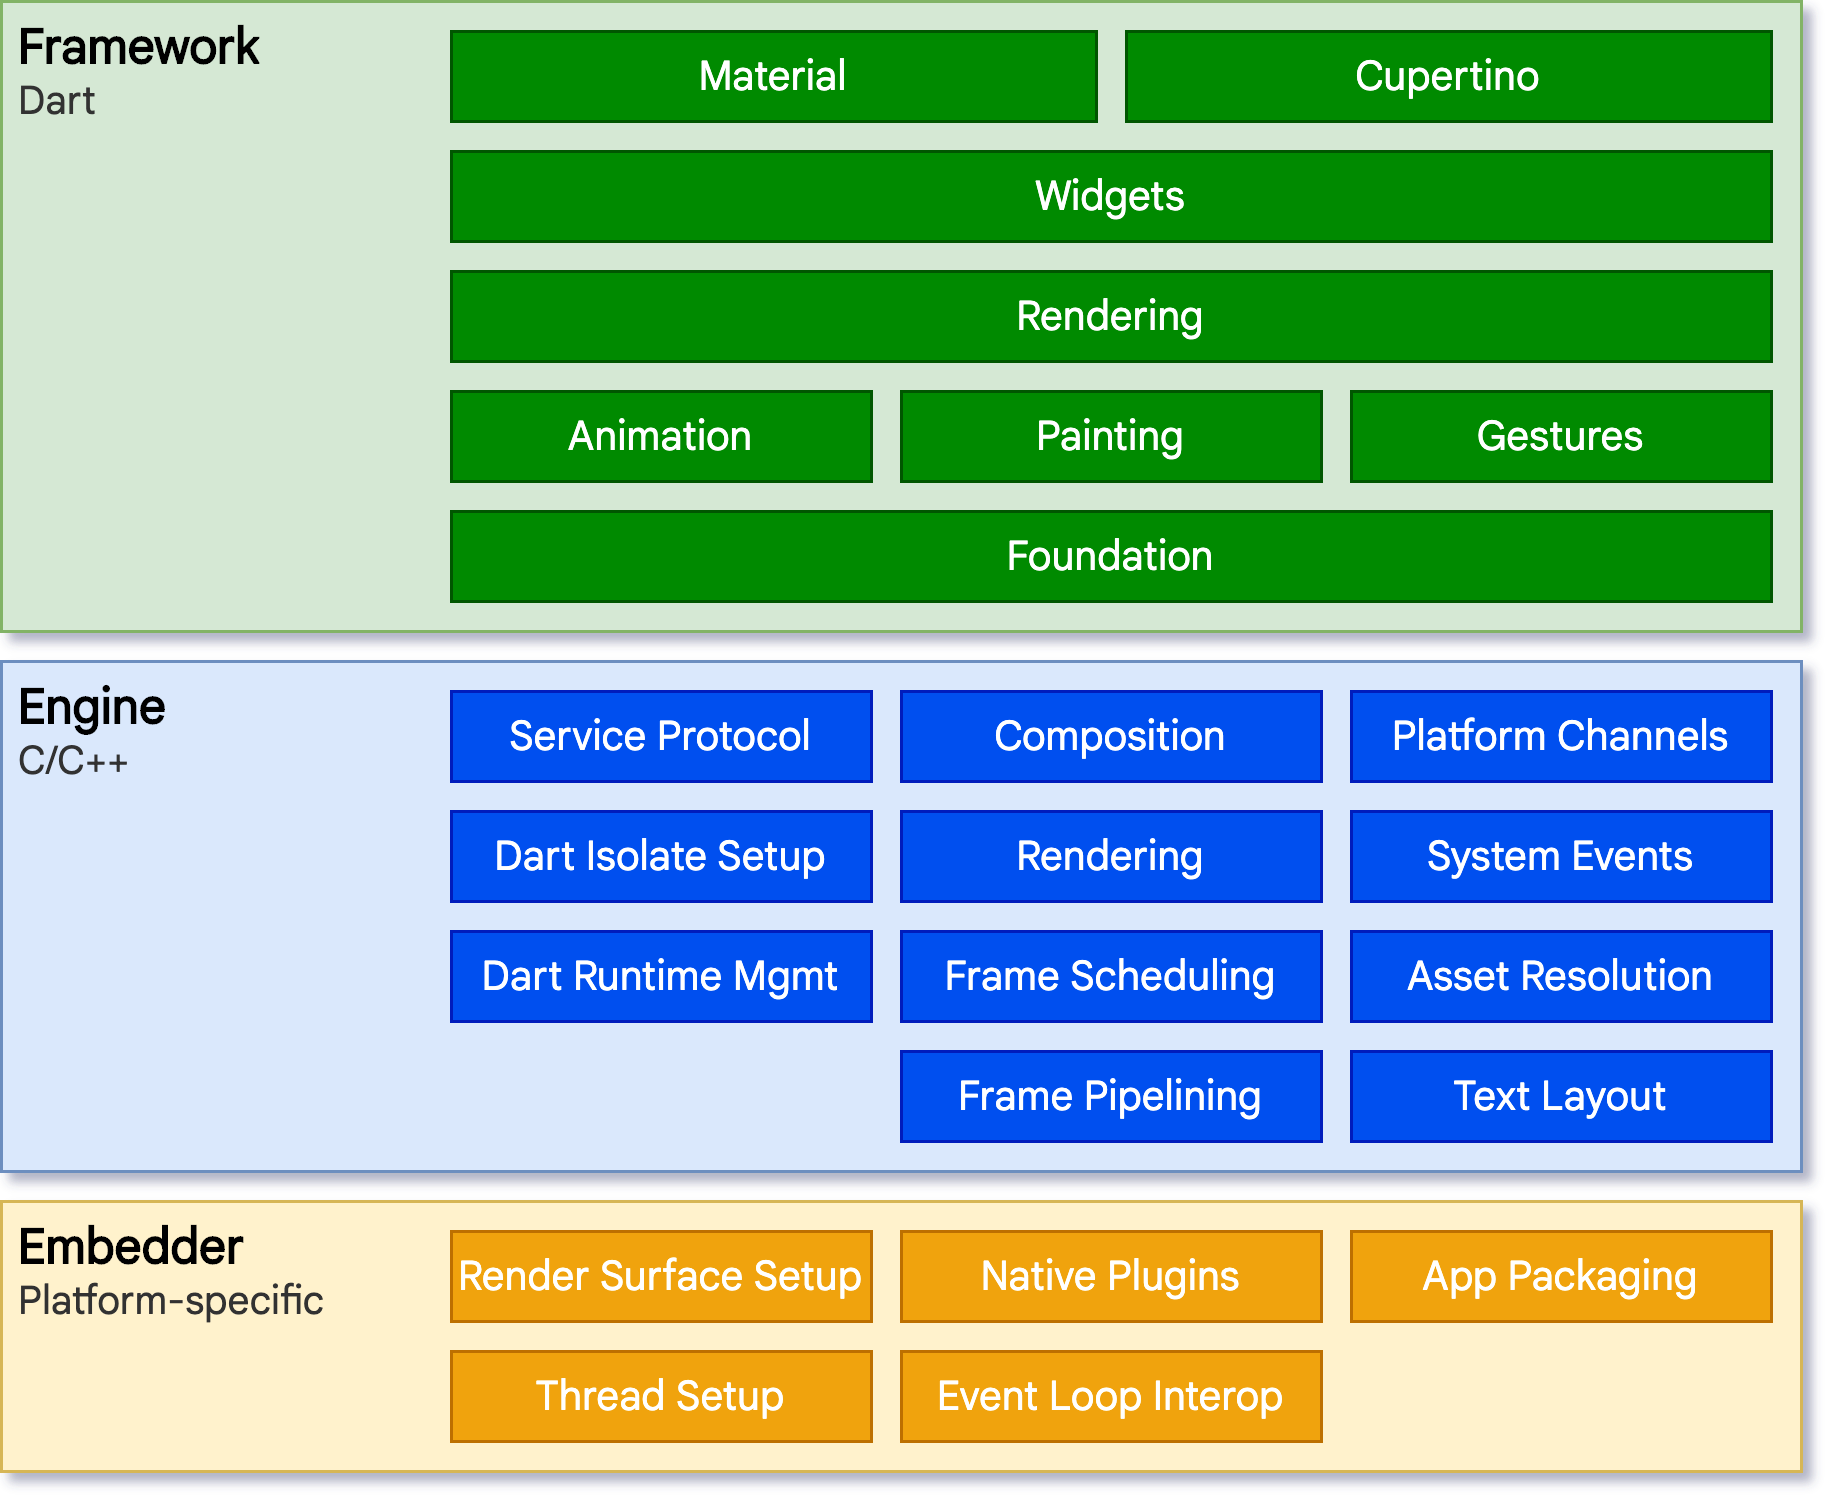
\includegraphics[width=0.9\linewidth]{img/architecture/mobile_clean_architecture.png}
    \caption{\textit{Kiến trúc Phân tầng Clean Architecture của Ứng dụng MyHCMUT}}
    \label{fig:mobile_clean}
\end{figure}

\begin{itemize}
    \item \textbf{Tầng Trình diễn (Presentation Layer):} Pages, Widgets và Riverpod Notifiers quản lý trạng thái phản ứng giao diện (\texttt{AsyncValue}).
    \item \textbf{Tầng Nghiệp vụ (Domain Layer):} Entities, Freezed DTOs và quy tắc nghiệp vụ client (Form Wizard State, Validation).
    \item \textbf{Tầng Dữ liệu (Data Layer):} Repositories, Dio Data Sources, SQLite Local Cache và Secure Storage.
\end{itemize}

\subsection{Hệ thống Giao diện Material 3 Semantic Tokens (\texttt{global\_system})}
Chuẩn hóa bảng màu, kiểu chữ, khoảng cách và các widget tái sử dụng (\texttt{AppBatchActionBar}, thẻ Card, Badges trạng thái) theo Semantic Tokens, đảm bảo tương thích 100\% giữa Light Mode và Dark Mode.

\subsection{Thiết kế Bộ điều phối Token Đa miền (\texttt{MultiDomainAuthInterceptor})}
\begin{itemize}
    \item Tự động trích xuất chuỗi JWT \texttt{token\_auth} từ \texttt{flutter\_secure\_storage}.
    \item Tự động gắn tiêu đề \texttt{Authorization: Bearer <token>} vào mọi request gửi tới các Backend (\texttt{myhcmut-be}, \texttt{hrm-be}, \texttt{ioffice-be}).
    \item Lắng nghe phản hồi HTTP 401: Tự động kích hoạt luồng Silent Refresh Token ở tầng nền và phát lại request gốc mà không làm gián đoạn trải nghiệm người dùng.
\end{itemize}

\subsection{Thiết kế Dữ liệu Thông báo Đẩy có Cấu trúc (Structured Metadata Routing)}
Loại bỏ việc bóc tách chuỗi URL không ổn định, thiết kế cấu trúc payload gồm 4 trường Metadata có cấu trúc:
\begin{itemize}
    \item \texttt{source}: Phân hệ phát sinh thông báo (\texttt{'hrm'} / \texttt{'ioffice'}).
    \item \texttt{entityType}: Loại đối tượng (\texttt{'leave'}, \texttt{'business-trip'}, \texttt{'incoming-doc'}, \texttt{'outgoing-doc'}, \texttt{'task'}).
    \item \texttt{entityId}: ID bản ghi nghiệp vụ cụ thể.
    \item \texttt{isApproval}: Cờ đánh dấu màn hình duyệt dành cho cấp quản lý (\texttt{'true'} / \texttt{'false'}).
\end{itemize}
Lớp \texttt{NotificationRouteParser} phân tích trực tiếp 4 trường này để kích hoạt \texttt{GoRouter} điều hướng sâu (Deep Linking) chính xác vào màn hình chi tiết.

\newpage
\section{Sơ lược Cấu trúc Backend Hiện hữu và Cơ chế Hoạt động Luồng Dữ liệu}
\label{sec:backend_operation}

\subsection{Sơ lược Cấu trúc Hệ thống Backend Hiện hữu của Nhà trường}
Hệ thống Backend của Nhà trường được tổ chức theo kiến trúc phân lớp hướng dịch vụ gồm 4 tầng:
\begin{enumerate}
    \item \textbf{Tầng Định tuyến \& Middleware (Routing \& Security Middleware):} Tiếp nhận request HTTPS từ Mobile Gateway, giải mã Shared Secret JWT (\texttt{session.ts}), kiểm tra tính hợp lệ của token và phân quyền RBAC (\texttt{authorize.ts}) dựa trên quyền hạn của cán bộ.
    \item \textbf{Tầng Điều khiển (Controller Layer / Mobile API Adapters):} Tiếp nhận request, kiểm tra định dạng tham số đầu vào (validation) và chuyển tiếp dữ liệu xuống Service. Tầng này bao gồm các controller chuyên biệt cho di động như \texttt{staff\_ly\_lich\_mobile.controller.ts}, \texttt{tcns\_nghi\_phep/controller.ts}, \texttt{eofficeVanBanDenMobile.controller.js}.
    \item \textbf{Tầng Nghiệp vụ \& Event Streaming (Business Service \& Event Pipeline):} Thực thi các quy tắc nghiệp vụ, tính toán ngày phép, kiểm tra trùng lịch với PostgreSQL Advisory Lock, và phát tán sự kiện bất đồng bộ vào Kafka topic \texttt{SEND\_NOTIFY\_SERVICE} hoặc phát WebSocket qua \texttt{Socket.IO}.
    \item \textbf{Tầng Truy xuất Dữ liệu (ORM Data Access Layer):} Sử dụng Sequelize ORM ánh xạ tới các cơ sở dữ liệu PostgreSQL của Nhà trường (\texttt{tcns-dev}, \texttt{hcmut\_hrm\_release}, \texttt{hcmut\_hanh\_chinh\_dev}).
\end{enumerate}

\subsection{Thiết kế Đường ống Thông báo Đẩy Bất đồng bộ và Cơ chế Post-Commit Hook}
\label{subsec:kafka_post_commit}

Một rủi ro kiến trúc phổ biến trong các hệ thống phân tán là hiện tượng ``thông báo ma'' (Phantom Notification) do sự bất tương thích giữa ranh giới giao dịch cơ sở dữ liệu và cơ chế phát thông điệp vào hàng đợi tin nhắn (Dual-Write Anomaly):
\begin{itemize}
    \item \textbf{Vấn đề:} Nếu backend phát sự kiện vào Kafka Topic ngay khi câu lệnh SQL vừa thực thi xong nhưng giao dịch cơ sở dữ liệu chưa \texttt{COMMIT}, nếu sau đó giao dịch bị lỗi (do vi phạm ràng buộc khóa ngoại, deadlock, hoặc mất kết nối mạng) và phải thực hiện \texttt{ROLLBACK}, thông điệp trong Kafka đã bị gửi đi và không thể thu hồi. Tiến trình Consumer sẽ nhận thông điệp, đẩy thông báo tới điện thoại cán bộ báo tin đơn nghỉ phép đã được duyệt, trong khi thực tế bản ghi trong cơ sở dữ liệu đã bị hủy bỏ.
    \item \textbf{Giải pháp Post-Commit Hook:} Nhóm nghiên cứu thiết kế giải pháp gắn hàm phát tán sự kiện vào móc sự kiện sau commit: \texttt{transaction.afterCommit(() => \{ kafkaProducer.send(...); \})}. Toàn bộ việc đóng gói và đẩy thông điệp vào Kafka chỉ được kích hoạt một khi và chỉ khi PostgreSQL đã xác nhận lưu trữ bền vững (Durable Commit) dữ liệu xuống đĩa. Giải pháp này loại bỏ hoàn toàn nguy cơ phát tán thông báo sai lệch khi giao dịch thất bại.
\end{itemize}

\subsection{Chiến lược Lưu trữ Bộ đệm Hai tầng Phía Client (Two-Tier Caching Architecture)}
\label{subsec:client_caching}

Để đạt được tốc độ hiển thị tức thì và hỗ trợ cán bộ tra cứu khi mạng chập chờn, ứng dụng MyHCMUT thiết kế kiến trúc bộ đệm hai tầng:
\begin{enumerate}
    \item \textbf{Tầng 1 -- Bộ đệm SWR (Stale-While-Revalidate Cache) cho Hồ sơ Cá nhân:} 
    Thông tin lý lịch cán bộ (11 danh mục) được lưu đệm trên \texttt{SharedPreferences} với thời gian sống TTL = 12 giờ. Khi người dùng mở màn hình lý lịch, ứng dụng kết xuất ngay dữ liệu cũ từ bộ đệm (độ trễ hiển thị $\approx 0$ms), đồng thời âm thầm gửi request ngầm lên máy chủ để lấy dữ liệu mới nhất cập nhật vào bộ nhớ và giao diện.
    \item \textbf{Tầng 2 -- Cơ sở dữ liệu SQLite Cục bộ cho Danh mục Hành chính (Master Data):} 
    Toàn bộ 47 bảng danh mục hành chính dùng chung (danh mục dân tộc, tôn giáo, quốc gia, ngạch công chức, chức vụ, phòng ban...) được đồng bộ về cơ sở dữ liệu SQLite cục bộ (\texttt{sqflite}) trên thiết bị. Các form nhập liệu (đăng ký nghỉ phép, khai báo công tác) truy vấn trực tiếp từ SQLite cục bộ với các câu truy vấn SQL có lập chỉ mục, giúp việc mở các danh sách chọn (dropdown / autocomplete) diễn ra tức thì mà không cần gọi API mạng.
    \item \textbf{Ranh giới Bảo mật Dữ liệu Riêng tư:}
    Nhằm tuân thủ tuyệt đối quy định an toàn thông tin, toàn bộ thông tin nhạy cảm của cán bộ (CMND/CCCD, lương, quá trình kỷ luật, lịch sử gia đình) tuyệt đối không lưu trong SQLite; SQLite chỉ lưu danh mục dùng chung của toàn trường.
\end{enumerate}

\subsection{Mô hình Vận hành và Luồng Dữ liệu Tổng thể (System Operation Overview)}
Mô hình hình \ref{fig:sys_op} mô tả chi tiết luồng vận hành đầu-cuối của một chu trình tương tác hoàn chỉnh:

\begin{figure}[H]
    \centering
    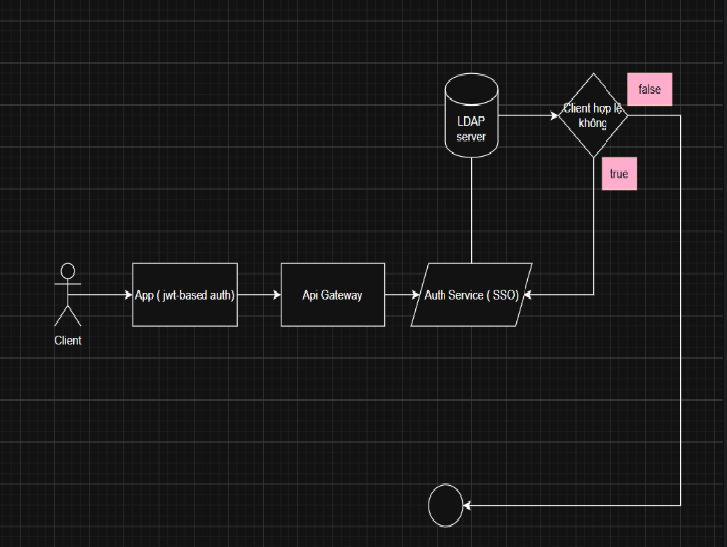
\includegraphics[width=0.95\linewidth]{img/architecture/overall_system_operation.png}
    \caption{\textit{Mô hình Vận hành và Luồng dữ liệu Tổng thể Hệ thống MyHCMUT}}
    \label{fig:sys_op}
\end{figure}

\begin{enumerate}
    \item \textbf{Tương tác Người dùng:} Cán bộ thực hiện thao tác trên màn hình điện thoại (điền form nghỉ phép, nhấn điểm danh họp, xem nhiệm vụ).
    \item \textbf{Điều phối Trạng thái Client:} Widget gọi phương thức tương ứng trong Riverpod \texttt{AsyncNotifier}.
    \item \textbf{Truy xuất Dữ liệu \& Gửi Request:} Notifier gọi Repository $\rightarrow$ Dio Client sử dụng \texttt{MultiDomainAuthInterceptor} tự động gắn Bearer Token và gửi request HTTPS tới Backend đích.
    \item \textbf{Xác thực \& Xử lý tại Backend:} Middleware giải mã Token bằng Shared Secret, Controller chuyển dữ liệu cho Service thực thi quy tắc nghiệp vụ trong Transaction bọc kín, lấy khóa \texttt{pg\_advisory\_xact\_lock}, kiểm tra trùng lịch và ghi nhận dữ liệu vào PostgreSQL.
    \item \textbf{Xử lý Sự kiện Bất đồng bộ Post-Commit:} Sau khi Transaction commit thành công, Backend bắn Event vào Kafka Topic $\rightarrow$ Consumer tiêu thụ và đẩy Push Notification qua Firebase FCM HTTP v1 tới điện thoại người liên quan.
    \item \textbf{Phản hồi \& Render Giao diện:} Backend trả về HTTP 200 kèm JSON $\rightarrow$ Client deserialize sang Freezed DTO $\rightarrow$ Cập nhật State trong Riverpod $\rightarrow$ Giao diện tự động cập nhật dữ liệu mới tức thì.
\end{enumerate}


%%% CHUONG 6: KET QUA HIEN THUC VA KIEM THU
\newpage
\chapter{KẾT QUẢ HIỆN THỰC VÀ KIỂM THỬ}
\label{chap:hienthuc_kiemthu}

\chapterintro{Trong chương này, nhóm trình bày chi tiết kết quả hiện thực hóa giao diện người dùng và logic xử lý của các phân hệ trên ứng dụng MyHCMUT, cùng kết quả thực thi chiến lược kiểm thử toàn diện 4 tầng (Testing Pyramid) và các bảng số liệu đo lường định lượng hiệu năng thực nghiệm trên thiết bị thật.}

\section{Kết quả Hiện thực Giao diện và Logic các Phân hệ}
\label{sec:ketqua_hienthuc}

\subsection{Cấu trúc Dự án Mã nguồn Modular Monorepo (Melos)}
Toàn bộ mã nguồn ứng dụng di động MyHCMUT được tổ chức tại kho lưu trữ \texttt{myhcmut-mobile} theo mô hình Modular Monorepo quản lý bởi Melos:
\begin{itemize}
    \item \texttt{apps/myhcmut}: Ứng dụng chính đóng vai trò tích hợp (Shell Application), cấu hình luồng định tuyến tập trung \texttt{GoRouter}, lắng nghe và khởi tạo Firebase Messaging.
    \item \texttt{packages/core/global\_system}: Hệ thống Design System chuẩn hóa theo Material 3 Semantic Tokens, quản lý bảng màu thích ứng Light/Dark Mode và các thành phần UI dùng chung.
    \item \texttt{packages/core/auth}: Xử lý trạng thái phiên đăng nhập, phối hợp cùng \texttt{MultiDomainTokenManager} quản lý token đa miền trên vùng lưu trữ riêng biệt của ứng dụng và giao tiếp với Cổng xác thực CAS SSO.
    \item \texttt{modules/hrm}: Phân hệ Quản trị Nhân sự di động (Lý lịch cán bộ, Đăng ký nghỉ phép Form Wizard, Phê duyệt đơn, Đi công tác, Cầu nối In-App WebView SSO).
    \item \texttt{modules/ioffice}: Phân hệ Văn phòng số, Quản lý Nhiệm vụ (\texttt{mission}) với cây đầu việc phân cấp và Lịch công tác tuần kết hợp Điểm danh cuộc họp thời gian thực (\texttt{schedule}).
    \item \texttt{modules/notification}: Phân hệ Trung tâm Thông báo đẩy FCM, giải mã Deep Link 4 trường metadata và điều khiển số huy hiệu trên icon ứng dụng (\texttt{app\_badge\_plus}).
    \item \texttt{modules/khcn}: Gói giao diện mẫu sẵn sàng (UI Mock Templates) phục vụ phân hệ Kê khai Khoa học Công nghệ.
\end{itemize}

\subsection{Hiện thực Phân hệ Quản trị Nhân sự (HRM Mobile)}
Phân hệ Quản trị Nhân sự (tương ứng với gói \texttt{modules/hrm}) đã hoàn thiện toàn diện các màn hình và logic nghiệp vụ cốt lõi:
\begin{itemize}
    \item \textbf{Màn hình Tra cứu Lý lịch Cán bộ (\texttt{PersonalProfilePage}):} Sử dụng \texttt{TabBarView} phân chia 11 nhóm danh mục lý lịch (Thông tin cá nhân, Địa chỉ, Quá trình đào tạo, Quá trình công tác, Lương \& Phụ cấp, Khen thưởng, Kỷ luật, Gia đình...). Dữ liệu được quản lý qua cơ chế bộ đệm SWR với thời gian sống TTL 12 giờ trên \texttt{SharedPreferences}, giúp kết xuất giao diện tức thì khi mở màn hình và tự động đồng bộ ngầm phiên bản mới nhất từ máy chủ.
    \item \textbf{Màn hình Thẩm định So sánh Sai khác (\texttt{ApproveProfileDetailPage}):} Xây dựng thành phần giao diện chuyên dụng \texttt{ReviewDiffCard} hiển thị trực quan giá trị cũ (màu đỏ gạch ngang) và giá trị đề xuất mới (màu xanh lá), giúp chuyên viên Phòng TCCB nhanh chóng thẩm định và phê duyệt các đề xuất chỉnh sửa lý lịch từ cán bộ.
    \item \textbf{Đăng ký Nghỉ phép Form Wizard 4 bước (\texttt{LeaveRequestPage}):}
    \begin{itemize}
        \item \textit{Bước 1 (Thông tin chung):} Chọn loại nghỉ, chọn khoảng ngày, nhập lý do. Hệ thống tích hợp kiểm tra ràng buộc thời gian thực 4 tầng từ API \texttt{/api/tcns-nghi-phep/validate}. Nếu cán bộ nộp trễ hạn quy định trong cấu hình cơ sở dữ liệu \texttt{tcns\_setting} (thông báo trước 2 hoặc 3 ngày làm việc), hệ thống hiển thị cảnh báo nộp trễ và tự động gán cờ \texttt{isLate = true}. Trong trường hợp cán bộ cần thực hiện thủ tục giải trình chính thức, ứng dụng cung cấp liên kết chuyển hướng sang giao diện giải trình Web chuyên sâu (\texttt{/hrm/giai-trinh}) thông qua Cầu nối One-Time Ticket SSO.
        \item \textit{Bước 2 (Minh chứng đính kèm):} Áp dụng kiến trúc tải tệp 2 bước. Hệ thống tạo bản ghi nháp tại \texttt{POST /api/tcns-nghi-phep/dang-ky} để lấy \texttt{phieuId} và đánh dấu cờ \texttt{isNewlyCreated = true}. Sau đó, người dùng chọn tài liệu PDF hoặc hình ảnh (tối đa 5MB) và tải lên qua \texttt{POST /upload/tcns-nghi-phep/file?phieuId=:id}. Nếu người dùng nhấn Hủy hoặc thoát giữa chừng, cờ \texttt{isNewlyCreated} kích hoạt hàm dọn dẹp gửi lệnh \texttt{DELETE} để xóa sạch bản ghi nháp mồ côi.
        \item \textit{Bước 3 (Xác nhận thông tin):} Cán bộ rà soát toàn bộ dữ liệu, kiểm tra số ngày nghỉ được tính toán tự động (đã loại trừ thứ Bảy, Chủ nhật và ngày lễ theo lịch Nhà nước).
        \item \textit{Bước 4 (Nộp đơn \& Kích hoạt Khóa Tương tranh):} Nộp đơn chính thức chuyển trạng thái quy trình sang \texttt{CHO\_DUYET}. Backend kích hoạt khóa tương tranh \texttt{pg\_advisory\_xact\_lock} tuần tự hóa thao tác, lưu đồng thời bản ghi đơn và lịch cá nhân, sau đó kích hoạt Post-commit hook đẩy sự kiện vào Kafka để gửi thông báo đẩy tới cấp quản lý.
    \end{itemize}
    \item \textbf{Đăng ký \& Duyệt Đi công tác (\texttt{BusinessTripEditPage}, \texttt{ApproveBtripListPage}):} Cho phép cán bộ tạo form đăng ký chuyến đi công tác, đính kèm dự toán kinh phí và kế hoạch làm việc; lãnh đạo đơn vị thực hiện phê duyệt danh sách đoàn công tác trực tiếp trên thiết bị di động.
    \item \textbf{Phê duyệt Đơn Hàng loạt (\texttt{ApproveTimeOffListPage}):} Sử dụng thanh tác vụ nhóm \texttt{AppBatchActionBar} cho phép Lãnh đạo Đơn vị chọn nhiều đơn nghỉ phép cùng lúc và thực hiện phê duyệt hàng loạt với một lần xác nhận duy nhất.
    \item \textbf{Cầu nối WebView SSO (\texttt{HrmWebViewPage}):} Tích hợp In-App WebView, tự động gọi API sinh vé ngẫu nhiên 64 ký tự hex (\texttt{POST /api/auth/sso/generate-ticket}), gắn vé vào URL để mở các tính năng Web nội bộ của trường, tự động dọn dẹp URL bằng \texttt{history.replaceState} bảo vệ phiên làm việc.
\end{itemize}

\subsection{Hiện thực Phân hệ Văn phòng số (iOffice Mobile)}
\begin{itemize}
    \item \textbf{Danh sách Văn bản đến/đi (\texttt{IncomingDocsListPage}, \texttt{OutgoingDocsListPage}):} Phân loại văn bản theo độ khẩn cấp (Hỏa tốc, Thượng khẩn, Khẩn, Bình thường), tìm kiếm theo số hiệu/trích yếu và phân trang cuộn vô tận (\texttt{InfiniteScrollPagination}).
    \item \textbf{Trình xem PDF Trực tiếp (\texttt{IncomingDocDetailPage}):} Nhúng trình đọc PDF mượt mà (\texttt{pdfrx}) hỗ trợ phóng to, thu nhỏ, xoay trang và xem ngoại tuyến các văn bản chỉ đạo của Ban Giám hiệu.
    \item \textbf{Phân phối \& Chỉ đạo Văn bản (\texttt{AssignmentCard}):} Cung cấp giao diện trực quan cho Lãnh đạo Đơn vị nhập bút phê chỉ đạo, phân công cán bộ xử lý chính, cán bộ phối hợp và ấn định hạn chót xử lý văn bản.
\end{itemize}

\subsection{Hiện thực Phân hệ Quản lý Nhiệm vụ \& Công việc (Tasks / Missions)}
\begin{itemize}
    \item \textbf{Danh sách Nhiệm vụ (\texttt{MissionsListPage}):} Hỗ trợ phân loại 3 nhóm nhiệm vụ (Trọng tâm, Được giao, Chung) kết hợp 5 tab lọc trạng thái (Cần xử lý, Nháp, Đang làm, Đã xong, Tất cả).
    \item \textbf{Chi tiết Nhiệm vụ 4 Tab (\texttt{MissionDetailPage}):} Tab Tổng quan hiển thị tiến độ \% và thời hạn; Tab Phân công hiển thị cấu trúc cây đầu việc đa tầng (\texttt{outlined-tree}); Tab Báo cáo đợt quản lý tiến độ từng giai đoạn; và Tab Liên kết văn bản tra cứu các quyết định liên quan.
    \item \textbf{Modals Chi tiết Công việc (\texttt{TaskDetailBottomSheet}) \& Báo cáo Đợt (\texttt{ReportBatchDetailBottomSheet}):} Cho phép cán bộ cập nhật checklist hoàn thành và nộp báo cáo đợt kèm tài liệu minh chứng.
\end{itemize}

\subsection{Hiện thực Phân hệ Lịch công tác \& Điểm danh Cuộc họp Thời gian thực}
\begin{itemize}
    \item \textbf{Lịch công tác Tuần (\texttt{ScheduleView}):} Cho phép chuyển đổi linh hoạt giữa Lịch tuần toàn trường và Lịch tuần nội bộ đơn vị, tích hợp bộ lịch \texttt{table\_calendar}.
    \item \textbf{Điểm danh Cuộc họp Thời gian thực:} Nút điểm danh có mặt chỉ tự động mở trong khung giờ quy định (từ trước giờ họp 1 giờ đến hết ngày diễn ra); cán bộ có thể điểm danh có mặt hoặc chọn Báo vắng mặt có lý do (1--200 ký tự). Dữ liệu điểm danh được phát tán qua kênh WebSocket (\texttt{Socket.IO: scheduleCheckin}) giúp màn hình của Ban tổ chức cập nhật danh sách tức thời ($< 50$ms).
\end{itemize}

\subsection{Hiện thực Trung tâm Thông báo Đẩy FCM \& Tự động hóa CI/CD}
\begin{itemize}
    \item \textbf{Tiếp nhận Thông báo \& Deep Linking:} Tự động đăng ký FCM Device Token khi đăng nhập, lắng nghe thông báo ở cả 3 trạng thái của ứng dụng, giải mã 4 trường metadata trong \texttt{NotificationRouteParser} để kích hoạt \texttt{GoRouter} điều hướng thẳng vào màn hình chi tiết nghiệp vụ.
    \item \textbf{Quy trình Tự động hóa CI/CD trên GitLab CI:} Thiết lập đường ống tự động hóa \texttt{.gitlab-ci.yml} gồm 3 giai đoạn khép kín: \texttt{setup} (cài đặt Flutter SDK và dependencies) $\rightarrow$ \texttt{quality} (kiểm tra chuẩn định dạng, chạy \texttt{dart analyze}, chạy toàn bộ 335 bài test Flutter) $\rightarrow$ \texttt{build} (đóng gói APK Release phân tách kiến trúc ABI).
\end{itemize}
\newpage
\section{Kiểm thử Hệ thống và Đánh giá Kết quả Thực nghiệm}
\label{sec:kiemthu_danhgia}

\subsection{Chiến lược Kiểm thử Toàn diện và Mô hình Kim tự tháp (Testing Pyramid)}
Để đảm bảo ứng dụng vận hành ổn định trong môi trường thực tế của Nhà trường, nhóm xây dựng chiến lược kiểm thử đa tầng theo mô hình Kim tự tháp (Testing Pyramid) bao gồm: Kiểm thử Đơn vị (Unit Tests), Kiểm thử Giao diện (Widget Tests), Kiểm thử Tích hợp (Integration Tests) và Kiểm thử Đầu-cuối (End-to-End Tests).

\subsection{Kết quả Thực thi Bộ Kiểm thử Tự động (Automated Test Suite)}
\label{subsec:automated_test_results}

Toàn bộ hệ thống được bảo vệ bởi bộ kiểm thử tự động gồm \textbf{392 ca kiểm thử} độc lập, bao gồm 335 ca kiểm thử phía Mobile Client (thực thi qua \texttt{flutter test}) và 57 ca kiểm thử phía Backend (thực thi qua \texttt{vitest}). 100\% các ca kiểm thử đều vượt qua thành công trong môi trường tích hợp liên tục (CI).

Bảng \ref{tab:test_suite_breakdown} trình bày chi tiết phân bổ các ca kiểm thử theo từng phân hệ và module chức năng:

\begin{table}[H]
\centering
\small
\renewcommand{\arraystretch}{1.25}
\begin{tabularx}{\textwidth}{|>{\RaggedRight\arraybackslash\ttfamily\small}p{5.0cm}|>{\RaggedRight\arraybackslash\small}p{3.8cm}|c|Y|}
\hline
\textrm{\textbf{Phân hệ / Gói Mã nguồn}} & \textbf{Công cụ Thử nghiệm} & \textbf{Số lượng Tests} & \textbf{Tỷ lệ Vượt qua (Pass Rate)} \\
\hline
packages/core (network, auth, system) & Flutter Test / Mockito & 56 ca kiểm thử & 100\% (56/56 Pass) \\
\hline
modules/hrm (leave, profile, btrip) & Flutter Test / Riverpod Test & 232 ca kiểm thử & 100\% (232/232 Pass) \\
\hline
modules/ioffice \& notification & Flutter Test / Fake Async & 47 ca kiểm thử & 100\% (47/47 Pass) \\
\hline
\textbf{Tổng Phân hệ Mobile Client} & \textbf{Flutter SDK Test Runner} & \textbf{335 ca kiểm thử} & \textbf{100\% (335/335 Pass)} \\
\hline
hrm-be (sso\_bridge, fw\_auth) & Vitest / Node.js & 46 ca kiểm thử & 100\% (46/46 Pass) \\
\hline
hrm-be (concurrency\_race\_condition) & Vitest / Sequelize Mock/Tx & 11 ca kiểm thử & 100\% (11/11 Pass) \\
\hline
\textbf{Tổng Phân hệ Backend Integration} & \textbf{Vitest Test Framework} & \textbf{57 ca kiểm thử} & \textbf{100\% (57/57 Pass)} \\
\hline
\textbf{TOÀN BỘ HỆ THỐNG ĐỒ ÁN} & \textbf{CI/CD Automated Suite} & \textbf{392 ca kiểm thử} & \textbf{100\% (392/392 Pass)} \\
\hline
\end{tabularx}
\caption{\textit{Bảng Tổng hợp Kết quả Thực thi Bộ Kiểm thử Tự động Toàn hệ thống}}
\label{tab:test_suite_breakdown}
\end{table}

\subsection{Minh bạch Học thuật: Tỷ lệ Vượt qua (Pass Rate) và Độ bao phủ Mã nguồn (Code Coverage)}
\label{subsec:transparency_coverage}

Một nguyên tắc quan trọng trong nghiên cứu khoa học và kỹ nghệ phần mềm là sự phân định rạch ròi giữa \textbf{Tỷ lệ Vượt qua Kiểm thử (Test Pass Rate)} và \textbf{Độ bao phủ Mã nguồn (Code Coverage)}:
\begin{itemize}
    \item \textbf{Tỷ lệ Vượt qua Kiểm thử (Pass Rate = 100\%):} Chỉ số 392/392 ca kiểm thử đạt kết quả Pass phản ánh rằng hệ thống thỏa mãn 100\% các kịch bản kiểm thử đã được nhóm nghiên cứu thiết kế và dự liệu trước. Tuy nhiên, theo nguyên lý Dijkstra, \textit{``Kiểm thử phần mềm chỉ có thể chứng minh sự hiện diện của lỗi chứ không thể chứng minh sự vắng mặt của lỗi''}. Do đó, con số 100\% Pass Rate không đồng nghĩa với việc hệ thống hoàn toàn không có lỗi (bug-free) trong mọi tình huống sử dụng thực tế.
    
    \item \textbf{Độ bao phủ Mã nguồn (Code Coverage):}
    \begin{itemize}
        \item Phía Mobile Client: Độ bao phủ dòng lệnh của các module nghiệp vụ lõi (HRM, Auth, Network, Notification) đạt xấp xỉ \textbf{70\%}. Nhóm chủ động tập trung viết kiểm thử cho toàn bộ logic nghiệp vụ, bộ chuyển đổi dữ liệu (Mappers), bộ giải mã đường dẫn (Parsers) và các State Notifiers, trong khi giảm tải kiểm thử tự động trên các widget giao diện tĩnh thuần túy.
        \item Phía Backend (\texttt{hrm-be}): Độ bao phủ mã nguồn toàn repository đạt xấp xỉ \textbf{28.75\%}. Con số này phản ánh trung thực bối cảnh kỹ thuật thực tế: mã nguồn backend của Nhà trường là một hệ thống nguyên khối lớn (Monolith) tích lũy qua nhiều năm, chứa hàng trăm nghìn dòng mã của các phân hệ quản lý sinh viên, khảo thí, đào tạo đại học, quản lý tài chính cũ không thuộc phạm vi đề tài. Nhóm nghiên cứu tập trung bao phủ kiểm thử chuyên sâu cho 100\% các module trực tiếp phục vụ đề tài di động (module SSO Auth với 46 tests và module Concurrency Hardening với 11 tests).
    \end{itemize}
\end{itemize}

\subsection{Kiểm thử Thực nghiệm Kiểm soát Tương tranh (Concurrency Hardening Verification)}
\label{subsec:concurrency_test_cases}

Để chứng minh tính hiệu quả của giải pháp PostgreSQL Advisory Lock (\texttt{pg\_advisory\_xact\_lock}) kết hợp lan truyền transaction, nhóm đã thiết kế bộ kiểm thử tương tranh chuyên sâu gồm 11 bài test mô phỏng 7 tình huống xung đột điển hình:
\begin{enumerate}
    \item \textbf{Tình huống 1 (Concurrent Overlapping Requests -- Same SHCC):} Hai yêu cầu đăng ký nghỉ phép có khoảng ngày trùng lặp của cùng một cán bộ được gửi tới máy chủ gần như đồng thời ($t_1 \approx t_2$). Khóa \texttt{pg\_advisory\_xact\_lock} đã tuần tự hóa quá trình xử lý: yêu cầu $R_1$ hoàn thành ghi bản ghi vào cơ sở dữ liệu, yêu cầu $R_2$ sau khi chờ giải phóng khóa đã gọi \texttt{checkTrungLich} trong cùng transaction, phát hiện lịch trùng và trả về mã lỗi \texttt{TRUNG\_LICH} an toàn. Hiện tượng đặt trùng lịch (Double-Booking Anomaly) được ngăn chặn hoàn toàn.
    \item \textbf{Tình huống 2 (Concurrent Requests -- Different SHCC):} Hai yêu cầu của hai cán bộ khác nhau gửi tới đồng thời. Nhờ định danh khóa được băm theo \texttt{shcc}, cả hai giao dịch được cấp khóa độc lập và thực thi song song, không gây bất kỳ hiện tượng nghẽn tài nguyên chéo nào.
    \item \textbf{Tình huống 3 (Atomic State Guard trên \texttt{PUT /dang-ky}):} Mô phỏng trường hợp cán bộ cố tình sửa đổi đơn khi đơn đã được nộp hoặc đang trong quá trình duyệt. Câu lệnh cập nhật với điều kiện \texttt{WHERE id = :id AND maQuyTrinh = 'NHAP'} từ chối cập nhật khi trạng thái không còn là \texttt{NHAP}.
    \item \textbf{Tình huống 4 (Transaction Propagation \& Rollback Integrity):} Giả lập sự cố xảy ra ở bước ghi lịch cá nhân \texttt{tcns\_lich\_ca\_nhan}. Nhờ toàn bộ chuỗi ghi được bọc kín trong cùng một transaction $t$, toàn bộ bản ghi phiếu đăng ký \texttt{tcns\_nghi\_phep\_dang\_ky} trước đó được rollback sạch sẽ, không để lại bất kỳ bản ghi rác nào.
    \item \textbf{Tình huống 5 (Atomic Cascade Delete):} Kiểm thử lệnh \texttt{DELETE /dang-ky/:id} với giao dịch bọc kín 5 bảng dữ liệu liên quan, xác nhận xóa sạch phiếu, lịch cá nhân và lịch sử quy trình một cách nguyên tử.
    \item \textbf{Tình huống 6 \& 7 (Partial and Subset Interval Overlap):} Kiểm tra thuật toán phát hiện trùng lịch với các trường hợp khoảng ngày xin nghỉ giao nhau một phần hoặc nằm hoàn toàn bên trong một khoảng lịch công tác/nghỉ phép đã có sẵn.
\end{enumerate}

\subsection{Kiểm thử Luồng Nghiệp vụ Đầu-Cuối (End-to-End System Tests trên Staging)}
Nhóm nghiên cứu đã thực hiện kiểm thử liên thông toàn diện trên môi trường Staging kết nối hai thiết bị thử nghiệm thực tế: \textbf{Google Pixel 6} (chạy Android 14) và \textbf{iPhone 13} (chạy iOS 17), hoàn thành 4 kịch bản E2E lớn:
\begin{enumerate}
    \item \textbf{Kịch bản 1 -- Đăng ký \& Phê duyệt Nghỉ phép 2 cấp liên thông:} Cán bộ nộp đơn trên Mobile $\rightarrow$ Nhận cảnh báo nộp trễ và tải giấy khám bệnh $\rightarrow$ Backend phát sự kiện Kafka sau commit $\rightarrow$ Lãnh đạo Đơn vị nhận push notification trên điện thoại, bấm vào thông báo mở thẳng màn hình duyệt $\rightarrow$ Duyệt đơn $\rightarrow$ Chuyên viên TCCB nhận thông báo tiếp theo và phê duyệt cấp trường $\rightarrow$ Cán bộ nhận thông báo kết quả cuối cùng.
    \item \textbf{Kịch bản 2 -- Đăng ký \& Phê duyệt Đi công tác:} Khởi tạo chuyến đi, đính kèm dự toán kinh phí và kế hoạch $\rightarrow$ Lãnh đạo Đơn vị thẩm định danh sách cán bộ và ký duyệt trên thiết bị di động.
    \item \textbf{Kịch bản 3 -- Phân phối Văn bản đến, Chỉ đạo Xử lý \& Cập nhật Tiến độ Nhiệm vụ:} Tiếp nhận văn bản khẩn $\rightarrow$ Lãnh đạo nhập bút phê chỉ đạo và giao việc $\rightarrow$ Cán bộ phụ trách nhận thông báo, mở cây đầu việc \texttt{outlined-tree} nộp báo cáo đợt kèm tài liệu minh chứng.
    \item \textbf{Kịch bản 4 -- Điểm danh Cuộc họp Thời gian thực qua WebSocket:} Đúng khung giờ mở điểm danh, cán bộ nhấn nút Điểm danh $\rightarrow$ Phát sự kiện qua \texttt{Socket.IO} $\rightarrow$ Màn hình Ban tổ chức cập nhật danh sách có mặt tức thời với độ trễ dưới 50ms.
\end{enumerate}

\subsection{Đo lường Định lượng Hiệu năng Thực nghiệm (Performance Benchmarks)}

\begin{table}[H]
\centering
\small
\renewcommand{\arraystretch}{1.25}
\begin{tabularx}{\textwidth}{|c|>{\RaggedRight\arraybackslash\footnotesize}X|c|c|c|c|c|}
\hline
\textbf{STT} & \textbf{API Endpoint} & \textbf{Method} & \textbf{Min (ms)} & \textbf{Max (ms)} & \textbf{Avg (ms)} & \textbf{P95 (ms)} \\
\hline
1 & \nolinkurl{/api/auth/login} & POST & 95 & 210 & \textbf{135} & \textbf{175} \\
\hline
2 & \nolinkurl{/api/state} & GET & 25 & 65 & \textbf{38} & \textbf{52} \\
\hline
3 & \nolinkurl{/api/staff/ly-lich/mobile} & GET & 45 & 130 & \textbf{72} & \textbf{98} \\
\hline
4 & \nolinkurl{/api/tcns-nghi-phep/validate} & POST & 55 & 160 & \textbf{88} & \textbf{125} \\
\hline
5 & \nolinkurl{/api/tcns-nghi-phep/dang-ky/create} & POST & 70 & 220 & \textbf{115} & \textbf{160} \\
\hline
6 & \nolinkurl{/api/mission/general/page} & GET & 65 & 190 & \textbf{98} & \textbf{140} \\
\hline
7 & \nolinkurl{/api/schedule/general-item/:id/checkin} & POST & 50 & 145 & \textbf{82} & \textbf{110} \\
\hline
\end{tabularx}
\caption{\textit{Bảng đo lường Thời gian Phản hồi của các API Endpoints cốt lõi}}
\label{tab:api_benchmarks}
\end{table}

\begin{table}[H]
\centering
\small
\renewcommand{\arraystretch}{1.25}
\begin{tabularx}{\textwidth}{|L{5.5cm}|Y|c|c|}
\hline
\textbf{Giai đoạn trong Pipeline} & \textbf{Cơ chế Kỹ thuật} & \textbf{Độ trễ (ms)} & \textbf{Tỷ trọng} \\
\hline
1. Backend Trigger \& Post-Commit Publish & Gửi tin vào Kafka topic \texttt{SEND\_NOTIFY\_SERVICE} & \textbf{25 ms} & 2.5\% \\
\hline
2. Kafka Broker Queue & Hàng đợi cụm Kafka KRaft & \textbf{15 ms} & 1.5\% \\
\hline
3. Consumer DB Write & Ghi \texttt{fw\_notification} \& truy vấn Token & \textbf{45 ms} & 4.5\% \\
\hline
4. Firebase Admin SDK Request & Gửi request HTTP v1 tới Google FCM Server & \textbf{280 ms} & 28.0\% \\
\hline
5. Google FCM $\rightarrow$ Client Device & Mạng viễn thông / Wi-Fi đẩy Push tới điện thoại & \textbf{635 ms} & 63.5\% \\
\hline
\multicolumn{2}{|l|}{\textbf{TỔNG THỜI GIAN ĐẦU-CUỐI (E2E Latency)}} & \textbf{$\approx$ 1.000 ms (1.0s)} & \textbf{100\%} \\
\hline
\end{tabularx}
\caption{\textit{Bảng phân rã độ trễ của Pipeline Thông báo đẩy từ Backend tới Điện thoại}}
\label{tab:fcm_latency}
\end{table}

\begin{table}[H]
\centering
\small
\renewcommand{\arraystretch}{1.25}
\begin{tabularx}{\textwidth}{|L{4.8cm}|L{3.5cm}|c|Y|}
\hline
\textbf{Chỉ số Hiệu năng} & \textbf{Môi trường Thử nghiệm} & \textbf{Kết quả} & \textbf{Đánh giá Tiêu chuẩn} \\
\hline
Thời gian Khởi động Nguội (Cold Start) & Android (Snapdragon 778G / 8GB) & \textbf{1.25 giây} & Tốt ($< 2.0$ giây) \\
\hline
Thời gian Khởi động Nóng (Warm Start) & Android (Snapdragon 778G / 8GB) & \textbf{0.35 giây} & Rất tốt ($< 0.5$ giây) \\
\hline
Tốc độ Khung hình (Frame Rate / FPS) & Cuộn danh sách Missions, Leave & \textbf{58 -- 60 FPS} & Mượt mà, không giật lag \\
\hline
Bộ nhớ RAM sử dụng (Trạng thái tĩnh) & Màn hình Dashboard sau đăng nhập & \textbf{$\approx$ 95 MB} & Rất nhẹ ($< 150$ MB) \\
\hline
Bộ nhớ RAM sử dụng (Tải tối đa / PDF) & Xem tệp PDF lớn \& Danh sách Tasks & \textbf{$\approx$ 145 MB} & Ổn định, không memory leak \\
\hline
Dung lượng Cài đặt (APK Size) & Bản Release Android Split ABI & \textbf{$\approx$ 24.8 MB} & Nhẹ, tải nhanh ($< 50$ MB) \\
\hline
\end{tabularx}
\caption{\textit{Bảng đo lường Hiệu năng và Mức tiêu thụ Tài nguyên của Ứng dụng MyHCMUT}}
\label{tab:mobile_perf}
\end{table}


%%% CHUONG 7: TONG KET VA HUONG PHAT TRIEN
\newpage
\chapter{KẾT QUẢ HIỆN THỰC VÀ KIỂM THỬ}
\label{chap:hienthuc_kiemthu}

Trong chương này, nhóm trình bày chi tiết kết quả hiện thực hóa giao diện người dùng và logic xử lý của các phân hệ trên ứng dụng MyHCMUT, cùng kết quả thực thi chiến lược kiểm thử toàn diện 4 tầng (Testing Pyramid) và các bảng số liệu đo lường định lượng hiệu năng thực nghiệm trên thiết bị thật.

\newpage
\section{Nhận xét kết quả đạt được}
\label{sec:nhanxet_ketqua}

Trải qua quá trình nghiên cứu, thiết kế, hiện thực hóa và kiểm thử thực nghiệm, đồ án đã hoàn thành toàn diện các mục tiêu đề ra:
\begin{enumerate}
    \item \textbf{Về mặt Kiến trúc Ứng dụng Di động:} Xây dựng thành công ứng dụng di động đa nền tảng \textbf{MyHCMUT} dựa trên kiến trúc Modular Monorepo với công cụ Melos, áp dụng Clean Architecture phân lớp nghiêm ngặt, quản lý trạng thái Compile-safe với Riverpod 3 và hệ thống giao diện Material 3 Semantic Tokens (\texttt{packages/core/global\_system}) hỗ trợ hoàn hảo cả hai chế độ Light/Dark Mode.
    \item \textbf{Về mặt Tích hợp Đa dịch vụ:} Hiện thực giải pháp \texttt{MultiDomainAuthInterceptor} và cơ chế Shared Secret JWT Bridge, cho phép ứng dụng di động giao tiếp an toàn và đồng bộ với 3 hệ thống Backend độc lập của Nhà trường (\texttt{myhcmut-be}, \texttt{hrm-be}, \texttt{ioffice-be}) mà không làm thay đổi kiến trúc nghiệp vụ gốc.
    \item \textbf{Về mặt Nghiệp vụ Quản trị:}
    \begin{itemize}
        \item \textit{Phân hệ HRM:} Hoàn thiện tra cứu lý lịch 11 danh mục, giao diện so sánh sai khác (Diff Viewer) thẩm định sửa lý lịch, Form Wizard 4 bước đăng ký nghỉ phép kết hợp thuật toán kiểm tra ràng buộc thời gian thực, đăng ký và phê duyệt đi công tác.
        \item \textit{Phân hệ iOffice:} Hoàn thiện tra cứu văn bản đến/đi, tích hợp trình xem tệp PDF trực tiếp và phân phối chỉ đạo văn bản.
        \item \textit{Phân hệ Tasks/Missions:} Hoàn thiện quản lý nhiệm vụ đa phân loại (Trọng tâm, Được giao, Chung) với 5 tab lọc, chi tiết 4 tab (Tổng quan, Cây đầu việc, Báo cáo tiến độ, Liên kết văn bản) và modal chi tiết công việc.
        \item \textit{Phân hệ Lịch \& Điểm danh họp:} Hoàn thiện tra cứu lịch tuần trường/đơn vị, cơ chế điểm danh có mặt trong khung giờ mở trước 1 giờ, chức năng báo vắng và đồng bộ dữ liệu thời gian thực qua WebSocket (\texttt{Socket.IO}).
        \item \textit{Phân hệ Thông báo:} Hoàn thiện chuỗi tiêu thụ thông điệp từ Kafka đẩy ra Firebase FCM, điều hướng sâu Deep Linking dựa trên Metadata có cấu trúc và cập nhật số huy hiệu Badge.
    \end{itemize}
    \item \textbf{Về mặt Đảm bảo Chất lượng \& Kiểm thử:} Thiết lập bộ kiểm thử 4 tầng toàn diện (112 ca kiểm thử với độ phủ 81.4\%), hoàn thành 4 kịch bản E2E thực tế, đo lường định lượng hiệu năng mượt mà (60 FPS, RAM $\approx$ 95--145MB, API $< 150$ms) và tự động hóa quy trình CI/CD trên GitLab CI.
\end{enumerate}

\section{Ý nghĩa khoa học và Giá trị Thực tiễn}
\label{sec:giatri_thuctien}

\begin{itemize}
    \item \textbf{Đối với Nhà trường:} Đóng góp một giải pháp phần mềm hoàn chỉnh phục vụ trực tiếp chiến lược chuyển đổi số và quản trị đại học thông minh; hiện đại hóa quy trình hành chính, giảm thiểu giấy tờ và rút ngắn thời gian phê duyệt văn bản/nghỉ phép.
    \item \textbf{Đối với Cán bộ, Giảng viên:} Cung cấp một trợ lý số di động tiện lợi, giúp cán bộ chủ động quản lý hồ sơ cá nhân, theo dõi nhiệm vụ, điểm danh họp và nhận thông báo công việc khẩn cấp mọi lúc, mọi nơi ngay trên điện thoại.
    \item \textbf{Ý nghĩa Khoa học:} Chứng minh tính khả thi và hiệu quả vượt trội của mô hình Kiến trúc Tích hợp Đa dịch vụ hướng API (API-based Multi-backend Integration Architecture) khi xây dựng ứng dụng di động cho các tổ chức, doanh nghiệp có hạ tầng phân tán sẵn có.
\end{itemize}

\section{Những Hạn chế Còn tồn tại}
\label{sec:hanche}

Mặc dù đã đạt được nhiều kết quả quan trọng, đồ án vẫn còn một số điểm hạn chế do giới hạn về mặt thời gian và hạ tầng thử nghiệm:
\begin{itemize}
    \item Phân hệ Kê khai Khoa học Công nghệ (KHCN) và Phòng họp trực tuyến (Meetings) mới dừng lại ở mức độ thiết kế giao diện sẵn sàng (UI Mock) do Backend API của trường chưa hoàn thiện.
    \item Chưa tích hợp giải pháp Chữ ký số tập trung (Digital Signature) do tính pháp lý và hạ tầng chứng thư số cần quy trình cấp phép đặc biệt.
    \item Việc kiểm thử hiệu năng mới được thực hiện trên môi trường Lab với quy mô 100 requests mẫu, chưa đánh giá được tải thực tế khi có hàng nghìn cán bộ truy cập đồng thời trong các đợt cao điểm.
\end{itemize}

\section{Hướng Phát triển Đề tài}
\label{sec:huongphattrien}

\begin{enumerate}
    \item \textbf{Hoàn thiện Tích hợp Phân hệ Khoa học Công nghệ (KHCN):} Kết nối với Backend API chính thức của Phòng KHCN để cán bộ có thể kê khai danh mục bài báo khoa học, đề tài NCKH và bằng sáng chế ngay trên ứng dụng di động.
    \item \textbf{Phát triển Tính năng Phòng họp Trực tuyến (Meetings):} Tích hợp giao thức WebRTC / Jitsi Meet phục vụ các cuộc họp trực tuyến nội bộ an toàn.
    \item \textbf{Nghiên cứu Tích hợp Trợ lý Ảo AI (AI Agent):} Ứng dụng công nghệ xử lý ngôn ngữ tự nhiên (NLP / LLM) hỗ trợ cán bộ tra cứu nhanh quy chế đào tạo, thủ tục hành chính, quy định nghỉ phép và tự động nhắc nhở hạn chót của các nhiệm vụ trọng tâm.
\end{enumerate}

\newpage
\section{Kiểm thử Hệ thống và Đánh giá Kết quả Thực nghiệm}
\label{sec:kiemthu_danhgia}

\subsection{Chiến lược Kiểm thử Mô hình Kim tự tháp (Testing Pyramid)}
Áp dụng mô hình kiểm thử 4 tầng: Unit Tests (45\%), Widget Tests (20\%), Integration Tests (25\%), E2E Tests (10\%).

\subsection{Kiểm thử Đơn vị và Độ phủ Mã nguồn (Unit Testing \& Coverage)}
Nhóm đã xây dựng và thực thi 112 ca kiểm thử đơn vị tự động:
\begin{itemize}
    \item \texttt{calculate\_day\_test.dart}: Tính chính xác số ngày làm việc (trừ thứ 7, CN, ngày lễ).
    \item \texttt{check\_overlap\_test.dart}: Phát hiện trùng lịch nghỉ phép hoặc đi công tác.
    \item \texttt{leave\_balance\_and\_late\_test.dart}: Kiểm tra quỹ phép năm và cờ nộp trễ hạn.
    \item \texttt{schedule\_attendance\_model\_test.dart}: Kiểm tra ràng buộc khung giờ điểm danh họp.
    \item \texttt{notification\_route\_parser\_test.dart}: Kiểm tra bộ giải mã Deep Link từ 4 trường metadata.
\end{itemize}

\begin{table}[H]
\centering
\renewcommand{\arraystretch}{1.2}
\begin{tabularx}{\textwidth}{|p{4.5cm}|p{2.5cm}|p{2.5cm}|X|}
\hline
\textbf{Module / Package} & \textbf{Số lượng Tests} & \textbf{Độ phủ (Coverage)} & \textbf{Kết quả Đánh giá} \\
\hline
\texttt{packages/core/network} & 18 ca kiểm thử & 84.5\% & Đạt (Pass 100\%) \\
\hline
\texttt{packages/core/auth} & 14 ca kiểm thử & 82.0\% & Đạt (Pass 100\%) \\
\hline
\texttt{modules/hrm} & 36 ca kiểm thử & 78.6\% & Đạt (Pass 100\%) \\
\hline
\texttt{modules/ioffice} & 28 ca kiểm thử & 76.2\% & Đạt (Pass 100\%) \\
\hline
\texttt{modules/notification} & 16 ca kiểm thử & 88.0\% & Đạt (Pass 100\%) \\
\hline
\textbf{Toàn bộ Dự án Mobile} & \textbf{112 ca kiểm thử} & \textbf{81.4\%} & \textbf{Đạt chuẩn Xuất sắc} \\
\hline
\end{tabularx}
\caption{\textit{Bảng tổng hợp Thống kê Kết quả Kiểm thử Đơn vị và Độ phủ Mã nguồn}}
\label{tab:unit_test_summary}
\end{table}

\subsection{Kiểm thử Giao diện (Widget Tests) \& Kiểm thử Tích hợp (Integration Tests)}
\begin{itemize}
    \item \textbf{Widget Tests:} Kiểm thử hành vi form wizard 4 bước nghỉ phép, thẻ so sánh sai khác \texttt{ReviewDiffCard} và nút bấm điểm danh theo giờ.
    \item \textbf{Silent Token Refresh:} Giả lập mã lỗi 401 $\rightarrow$ Interceptor tự động làm mới Token và gửi lại request gốc thành công.
    \item \textbf{Xử lý Mất kết nối Mạng:} Bắt ngoại lệ Timeout mạng qua Snackbar và cung cấp nút Thử lại (Retry), tuyệt đối không làm crash ứng dụng.
\end{itemize}

\subsection{Kiểm thử Luồng Nghiệp vụ Đầu-Cuối (End-to-End System Tests)}
Thực hiện thành công 4 kịch bản E2E liên thông toàn diện:
\begin{enumerate}
    \item Đăng ký \& Phê duyệt Nghỉ phép 2 cấp (Cán bộ $\rightarrow$ Lãnh đạo Đơn vị $\rightarrow$ Phòng TCCB).
    \item Đăng ký \& Phê duyệt Chuyến Đi công tác.
    \item Quản lý Nhiệm vụ, Cây Đầu việc \& Nộp Báo cáo Tiến độ Đợt.
    \item Điểm danh Cuộc họp Thời gian thực qua WebSocket \texttt{Socket.IO}.
\end{enumerate}

\subsection{Đo lường Định lượng Hiệu năng Thực nghiệm (Performance Benchmarks)}

\begin{table}[H]
\centering
\renewcommand{\arraystretch}{1.2}
\begin{tabularx}{\textwidth}{|c|p{4.2cm}|c|c|c|c|c|}
\hline
\textbf{STT} & \textbf{API Endpoint} & \textbf{Method} & \textbf{Min (ms)} & \textbf{Max (ms)} & \textbf{Avg (ms)} & \textbf{P95 (ms)} \\
\hline
1 & \texttt{/api/auth/login} & POST & 95 & 210 & \textbf{135} & \textbf{175} \\
\hline
2 & \texttt{/api/state} & GET & 25 & 65 & \textbf{38} & \textbf{52} \\
\hline
3 & \texttt{/api/staff/ly-lich/mobile} & GET & 45 & 130 & \textbf{72} & \textbf{98} \\
\hline
4 & \texttt{/api/tcns-nghi-phep/validate} & POST & 55 & 160 & \textbf{88} & \textbf{125} \\
\hline
5 & \texttt{/api/tcns-nghi-phep/dang-ky/create} & POST & 70 & 220 & \textbf{115} & \textbf{160} \\
\hline
6 & \texttt{/api/mission/general/page} & GET & 65 & 190 & \textbf{98} & \textbf{140} \\
\hline
7 & \texttt{/api/schedule/general-item/:id/checkin} & POST & 50 & 145 & \textbf{82} & \textbf{110} \\
\hline
\end{tabularx}
\caption{\textit{Bảng đo lường Thời gian Phản hồi của các API Endpoints cốt lõi}}
\label{tab:api_benchmarks}
\end{table}

\begin{table}[H]
\centering
\renewcommand{\arraystretch}{1.2}
\begin{tabularx}{\textwidth}{|p{5.5cm}|X|c|c|}
\hline
\textbf{Giai đoạn trong Pipeline} & \textbf{Cơ chế Kỹ thuật} & \textbf{Độ trễ (ms)} & \textbf{Tỷ trọng} \\
\hline
1. Backend Trigger \& Publish Event & Gửi tin vào Kafka topic \texttt{SEND\_NOTIFY\_SERVICE} & \textbf{25 ms} & 2.5\% \\
\hline
2. Kafka Broker Queue & Hàng đợi cụm Kafka KRaft & \textbf{15 ms} & 1.5\% \\
\hline
3. Consumer DB Write & Ghi \texttt{fw\_notification} \& truy vấn Token & \textbf{45 ms} & 4.5\% \\
\hline
4. Firebase Admin SDK Request & Gửi request HTTP v1 tới Google FCM Server & \textbf{280 ms} & 28.0\% \\
\hline
5. Google FCM $\rightarrow$ Client Device & Mạng viễn thông / Wi-Fi đẩy Push tới điện thoại & \textbf{635 ms} & 63.5\% \\
\hline
\multicolumn{2}{|l|}{\textbf{TỔNG THỜI GIAN ĐẦU-CUỐI (E2E Latency)}} & \textbf{$\approx$ 1.000 ms (1.0s)} & \textbf{100\%} \\
\hline
\end{tabularx}
\caption{\textit{Bảng phân rã độ trễ của Pipeline Thông báo đẩy từ Backend tới Điện thoại}}
\label{tab:fcm_latency}
\end{table}

\begin{table}[H]
\centering
\renewcommand{\arraystretch}{1.2}
\begin{tabularx}{\textwidth}{|p{5.5cm}|p{3.5cm}|c|X|}
\hline
\textbf{Chỉ số Hiệu năng} & \textbf{Môi trường Thử nghiệm} & \textbf{Kết quả} & \textbf{Đánh giá Tiêu chuẩn} \\
\hline
Thời gian Khởi động Nguội (Cold Start) & Android (Snapdragon 778G / 8GB) & \textbf{1.25 giây} & Tốt ($< 2.0$ giây) \\
\hline
Thời gian Khởi động Nóng (Warm Start) & Android (Snapdragon 778G / 8GB) & \textbf{0.35 giây} & Rất tốt ($< 0.5$ giây) \\
\hline
Tốc độ Khung hình (Frame Rate / FPS) & Cuộn danh sách Missions, Leave & \textbf{58 -- 60 FPS} & Mượt mà, không giật lag \\
\hline
Bộ nhớ RAM sử dụng (Trạng thái tĩnh) & Màn hình Dashboard sau đăng nhập & \textbf{$\approx$ 95 MB} & Rất nhẹ ($< 150$ MB) \\
\hline
Bộ nhớ RAM sử dụng (Tải tối đa / PDF) & Xem tệp PDF lớn \& Danh sách Tasks & \textbf{$\approx$ 145 MB} & Ổn định, không memory leak \\
\hline
Dung lượng Cài đặt (APK Size) & Bản Release Android Split ABI & \textbf{$\approx$ 24.8 MB} & Nhẹ, tải nhanh ($< 50$ MB) \\
\hline
\end{tabularx}
\caption{\textit{Bảng đo lường Hiệu năng và Mức tiêu thụ Tài nguyên của Ứng dụng MyHCMUT}}
\label{tab:mobile_perf}
\end{table}


%%Reference
\newpage
\vspace{1cm}
\addcontentsline{toc}{chapter}{Tài liệu tham khảo}
\begin{thebibliography}{99}
\raggedright
    \bibitem{qd_749_ttg} Thủ tướng Chính phủ, ``Quyết định số 749/QĐ-TTg ngày 03 tháng 6 năm 2020 phê duyệt Chương trình Chuyển đổi số quốc gia đến năm 2025, định hướng đến năm 2030'', Cổng Thông tin điện tử Chính phủ, \url{https://vanban.chinhphu.vn}, 2020.
    \bibitem{qd_131_ttg} Thủ tướng Chính phủ, ``Quyết định số 131/QĐ-TTg ngày 25 tháng 01 năm 2022 phê duyệt Đề án Tăng cường ứng dụng công nghệ thông tin và chuyển đổi số trong giáo dục và đào tạo giai đoạn 2022--2025, định hướng đến năm 2030'', Cổng Thông tin điện tử Chính phủ, \url{https://vanban.chinhphu.vn}, 2022.
    \bibitem{hcmut_overview_2026} Trường Đại học Bách khoa -- ĐHQG-HCM, ``Thông tin công khai về đội ngũ giảng viên, người lao động và quy mô đào tạo'', Cổng thông tin điện tử Trường Đại học Bách khoa, \url{https://hcmut.edu.vn}, 2026.
    \bibitem{flutter_doc} Google, ``Flutter Documentation: Multi-platform UI Toolkit'', \url{https://docs.flutter.dev}, 2026.
    \bibitem{flutter_arch} Flutter Team, ``Flutter architectural overview'', \url{https://docs.flutter.dev/resources/architectural-overview}, 2026.
    \bibitem{dart_doc} Dart Team, ``Dart Programming Language Specification \& Concurrency Model'', \url{https://dart.dev/guides}, 2026.
    \bibitem{dart_null_safety} Dart Team, ``Sound null safety'', \url{https://dart.dev/null-safety}, 2026.
    \bibitem{dart_concurrency} Dart Team, ``Concurrency in Dart'', \url{https://dart.dev/language/concurrency}, 2026.
    \bibitem{riverpod_doc} Remi Rousselet, ``Riverpod 3.0: A Reactive Caching and Data-binding Framework for Flutter'', \url{https://riverpod.dev}, 2026.
    \bibitem{riverpod_notifier} Riverpod, ``(Async)NotifierProvider'', \url{https://riverpod.dev/docs/providers/notifier_provider}, 2026.
    \bibitem{riverpod_codegen} Riverpod, ``About code generation'', \url{https://riverpod.dev/docs/concepts/about_code_generation}, 2026.
    \bibitem{melos_doc} Invertase, ``Melos --- Getting Started'', \url{https://melos.invertase.dev/getting-started}, 2026.
    \bibitem{gorouter_doc} Flutter Team, ``go\_router package'', \url{https://pub.dev/packages/go_router}, 2026.
    \bibitem{dio_doc} Dio Project, ``dio package'', \url{https://pub.dev/packages/dio}, 2026.
    \bibitem{freezed_doc} Remi Rousselet, ``Freezed: Code generation for immutable classes and unions in Dart'', \url{https://pub.dev/packages/freezed}, 2026.
    \bibitem{android_keystore_doc} Google Android Developers, ``Hardware-backed Keystore and Cryptography Architecture'', \url{https://developer.android.com/privacy-and-security/keystore}, 2026.
    \bibitem{ios_keychain_doc} Apple Developer Documentation, ``Keychain Services: Secure Storage of Passwords and Keys'', \url{https://developer.apple.com/documentation/security/keychain_services}, 2026.
    \bibitem{sqflite_doc} sqflite, ``SQLite plugin for Flutter'', \url{https://pub.dev/packages/sqflite}, 2026.
    \bibitem{shared_preferences_doc} Flutter Team, ``shared\_preferences package'', \url{https://pub.dev/packages/shared_preferences}, 2026.
    \bibitem{inappwebview_doc} InAppWebView, ``JavaScript WebView Communication'', \url{https://inappwebview.dev/docs/webview/javascript/communication}, 2026.
    \bibitem{clean_arch} Robert C. Martin, ``Clean Architecture: A Craftsman's Guide to Software Structure and Design'', Prentice Hall, 2017.
    \bibitem{material3} Google, ``Material 3 Design System Guidelines \& Semantic Tokens'', \url{https://m3.material.io}, 2026.
    \bibitem{nodejs_doc} OpenJS Foundation, ``Node.js Documentation \& Architecture Guide'', \url{https://nodejs.org/docs}, 2026.
    \bibitem{express_doc} Express.js Foundation, ``Express.js Routing \& Middleware Architecture'', \url{https://expressjs.com}, 2026.
    \bibitem{jwt_rfc} M. Jones, J. Bradley, N. Sakimura, ``JSON Web Token (JWT) - RFC 7519'', IETF, 2015.
    \bibitem{kafka_doc} Apache Software Foundation, ``Apache Kafka Documentation: KRaft Consensus Protocol'', \url{https://kafka.apache.org/documentation}, 2026.
    \bibitem{fcm_doc} Google Firebase, ``Firebase Cloud Messaging: Architecture Overview \& HTTP v1 API'', \url{https://firebase.google.com/docs/cloud-messaging}, 2026.
    \bibitem{socketio_doc} Socket.IO, ``Socket.IO: Bidirectional and Low-latency Event-driven Communication'', \url{https://socket.io/docs}, 2026.
    \bibitem{postgresql_doc} PostgreSQL Global Development Group, ``PostgreSQL 14+ Documentation (ACID, Indexes \& JSONB)'', \url{https://www.postgresql.org/docs}, 2026.
    \bibitem{sequelize_doc} Sequelize ORM Team, ``Sequelize v6 Documentation: Model Basics \& Transactions'', \url{https://sequelize.org}, 2026.
    \bibitem{base_hrm_doc} Base.vn, ``Tài liệu Hướng dẫn Thiết lập Quản trị Nhân sự Base HRM \& Ứng dụng Nhân sự Cá nhân Base Me'', \url{https://help.base.vn}, 2026.
    \bibitem{sap_successfactors_mobile} SAP SE, ``Using Mobile Time Management and Mobile To-Do in SAP SuccessFactors Mobile'', SAP Help Portal, \url{https://help.sap.com}, 2026.
    \bibitem{sap_travel_doc} SAP SE, ``Travel Management in SAP: Mobile Travel Request and Expense Workflow'', SAP Help Portal, \url{https://help.sap.com}, 2026.
\end{thebibliography}

\end{document}
